\documentclass[12pt, a4paper]{report}

% Packages
\usepackage[utf8]{inputenc}
\usepackage{amsmath, amssymb}
\usepackage{listings}
\usepackage{amsthm} 
\usepackage{algorithm}
\usepackage{algpseudocode}
\usepackage{graphicx}
\usepackage[]{xcolor}
\usepackage{hyperref}
\usepackage{caption}
\usepackage{float}
\usepackage{booktabs}
\usepackage{tabularx}
\usepackage{array}
\usepackage{geometry}
\usepackage{setspace}
\usepackage{times} % Times New Roman font
\usepackage{titlesec}
\usepackage{pifont}
\usepackage{tikz}
\usetikzlibrary{calc}
\usepackage[backend=biber, style=numeric, sorting=ynt]{biblatex}

\captionsetup{
	font=small,             
	labelfont=bf,
	textfont={color=gray!100} 
}

% Geometry package for setting margins
\geometry{
  left=2.5cm,
  right=2.5cm,
  top=2.5cm,
  bottom=2.5cm,
}

% for setting codes
\lstset{
	backgroundcolor=\color{gray!10},    
	basicstyle=\ttfamily\small,         
	commentstyle=\color{green!50!black}, 
	keywordstyle=\color{blue},          
	stringstyle=\color{red},            
	showstringspaces=false,             
	numbers=left,                       
	captionpos=b,                       
	frame=single,                       
	breaklines=true,                    
}
%------------------------------------------------------------------------------------

%------------------------------------------------------------------------------------
\titleformat{\chapter}[display]
  {\normalfont\LARGE\bfseries}{\chaptertitlename\ \thechapter}{20pt}{\Huge}
\titleformat{\section}
{\normalfont\Large\bfseries}
{\thesection}{1em}{}
\titleformat{\subsection}
{\normalfont\Large\bfseries}
{\thesubsection}{1em}{}
\titleformat{\subsubsection}
{\normalfont\large\bfseries}
{\thesubsubsection}{1em}{}
\DeclareCaptionFont{}{}
\captionsetup{labelfont={bf}}

\newcommand{\RNum}[1]{\uppercase\expandafter{\romannumeral #1\relax}}

\addbibresource{ref.bib}

% Line spacing
\onehalfspacing

\theoremstyle{definition}
\newtheorem{definition}{Definition}[chapter]

\theoremstyle{plain}
\newtheorem{theorem}{Theorem}[chapter]
\newtheorem{lemma}[theorem]{Lemma}

\theoremstyle{remark}
\newtheorem{remark}{Remark}[chapter]


% Title Page
\begin{document}
\title{THESIS TITLE}
\author{Alberto Trashaj}
\date{2023}

%----------------------------- Frontispiece
\newgeometry{margin=0.8in}
\begin{titlepage}
    \begin{center}
        \vspace*{0.2cm}
        {\fontsize{19pt}{20pt}\selectfont \textbf{Alma Mater Studiorum - Università di Bologna}\par}
    
        \noindent\hrulefill
        \vspace{0.8cm}
        
        \Large
        
        Departement of Statistical Science \\
        Second Cycle Degree in Statistical Sciences
        
        
        
        \Large
        \vspace{5cm}
        {\fontsize{22.5pt}{22.5}{\textbf{Comparative Analysis of Music Clustering and Classification Using Audio Feature Extraction and Time Series Analysis}}}

        
     
        \vspace{4.5cm}
         \begin{minipage}[t]{0.48\textwidth}
        \begin{flushleft}
            {\fontsize{16pt}{16pt}\textbf{Presented by:} \\ Sixun Che \\ \textbf{Matricola:} \\ 0001133202}
        \end{flushleft}
    \end{minipage} 
    \begin{minipage}[t]{0.48\textwidth}
        \begin{flushright}
            {\fontsize{16pt}{16pt}\textbf{Supervisor:} \\ Prof. Matteo Farnè}
        \end{flushright}
    \end{minipage}
        
        
        \vfill
        \noindent\hrulefill
        \vspace{0.3cm}
        \Large
        
       
        
        \RNum{1} \RNum{2} or \RNum{3} SESSION \\
        Academic Year 2024/2025
    \end{center}
\end{titlepage}
\restoregeometry
\vspace*{5cm}
\begin{flushright}
  {\parbox{4.2cm}{\textit{}}}
\end{flushright}

% Abstract
\begin{abstract}
\noindent
"Lorem ipsum dolor sit amet, consectetur adipiscing elit, sed do eiusmod tempor incididunt ut labore et dolore magna aliqua. Ut enim ad minim veniam, quis nostrud exercitation ullamco laboris nisi ut aliquip ex ea commodo consequat. Duis aute irure dolor in reprehenderit in voluptate velit esse cillum dolore eu fugiat nulla pariatur. Excepteur sint occaecat cupidatat non proident, sunt in culpa qui officia deserunt mollit anim id est laborum."\\
\textbf{Keywords:} Classification, Clustering, Time Series, Feature Project, Music
\end{abstract}


% Table of Contents
\tableofcontents

% Main Content
\chapter{Introduction}
\section{Background}
The relationship between music and mathematics has a rich and ancient history, tracing back thousands of years to the time of the Greek philosopher Pythagoras. He is often credited with being the first one to observe the deep connection between numerical ratios and musical harmony. According to a famous story recorded by Nicomachus, Pythagoras once passed by a blacksmith’s shop and noticed that the sounds produced by hammers striking metal differed in pitch. He discovered that the variation in pitch was not random but corresponded to the weight ratios of the hammers. This observation led him to further investigate the properties of sound and string vibrations. He found that when the lengths of strings were in simple integer ratios—such as 2:1, 3:2, or 4:3—they produced harmonious intervals that were naturally pleasing to the ear. From this, Pythagoras concluded that musical harmony is fundamentally rooted in numerical relationships, and that numbers are the essence of musical beauty.\\
\\
Fast forward to the modern era, and the influence of mathematics on music has grown even more profound with the advent of digital technology. Innovations in audio engineering and computer science have revolutionized the way we store, process, and reproduce sound. Complex signals, which are inherently analog and continuous, can now be captured and transformed into digital formats such as WAV, MP3, FLAC, and many others. This transformation is made possible through sophisticated encoding algorithms that break down audio into numerical representations, allowing sound to be stored as sequences of time-based data.\\
\\
In essence, these modern technologies have brought Pythagoras's vision to life in a completely new way. Every piece of music—whether it's a delicate solo piano piece, a powerful orchestral symphony, a deep bassline, or a sharp cymbal crash—can now be represented as a stream of numerical data. Through a process called sampling, recording devices convert continuous sound waves into discrete digital samples, taken at fixed intervals known as the sample rate (commonly 22.05 kHz or 44.1 kHz). These samples capture the amplitude of the sound wave at each point in time, resulting in a digital approximation of the original sound. The final outcome is a sequence of numbers that, when processed and played back, can faithfully reproduce the rich, dynamic experience of live music.\\
\\
The time series form of audio data not only preserves the temporal structure of sound but also provides a solid foundation for mathematical and statistical analysis. By applying techniques like the Fourier transform, we can break down complex audio signals into their frequency components, enabling a deeper understanding of the sound’s characteristics. Machine learning algorithms can be trained on this data to recognize musical styles, classify genres or detect patterns. Furthermore, with the rise of AIGC (Artificial Intelligence Generated Content), we can even create entirely new pieces of music by learning from existing audio datasets. In this way, time series data serves as a vital bridge between the physical world of sound and the digital realm of computation.\\
\\
As far as we know music can be reckoned as various genres. A piece of music from a special kind of genre sharing its unique style, the rhythm, rhyme, tone and etc. are all different. Therefore, as the core element of music classification system, genre has irreplaceable important value in music creation, communication, consumption and research. In essence, the identification of musical genres is not only a simple classification label, but also a structural expression of human musical cognitive system, reflecting the musical aesthetic paradigm formed under the specific historical and cultural background. The importance of music genre is first reflected in its guiding role in music creation practice. Each mature music genre represents a complete music grammar system formed through long-term development, including specific technical specifications such as harmonic progression, rhythm pattern, musical structure, orchestration, etc. For example, the sonata form in classical music, the improvised paragraph in jazz, and the synthesizer timbre design in electronic music are the core features of the corresponding genres. These norms not only provide a referential framework for creators, but also ensure the continuity of music culture through intergenerational inheritance. In the field of music education, genre system forms the basis of systematic teaching. Music colleges usually divide professional directions according to genre. This classification method can help students establish a clear knowledge map and more effectively master music language of a specific style.\\
\\
From the perspective of industrial economy, music genre is the key dimension of market segmentation. Record companies, streaming media platforms and performance markets all rely heavily on genre classification to develop business strategies. According to statistics, Spotify, the world's largest music streaming media service platform, uses more than 5000 genre tags to optimize its recommendation algorithm. This refined classification is directly related to the music consumption market of billions of dollars every year. The commercial value of music genre is also reflected in its close binding with specific consumer groups. Audiences of different ages and cultural backgrounds often show obvious genre preferences. In the digital music era, genre tags have become the basic unit of big data analysis. The platform can not only achieve accurate recommendations, but also predict market trends and guide the creation direction of new works through the genre preference data of users.\\
\\
At the academic research level, music schools provide a systematic analytical framework for musicology research. Musicians can reveal the internal law of music development by comparing the morphological characteristics of different schools. For example, through the comparative study of music schools from the Baroque period to the classical period, scholars have clearly combed out the evolution track of the functional harmony system. In the field of cognitive psychology, music genre research helps scientists understand the mechanism of human auditory perception, and experiments have proved that the audience's brain produces distinctive neural response patterns to concerts of different genres. These research results not only deepen our understanding of the nature of music, but also provide theoretical support for music therapy and other application fields.\\
\\
From the perspective of technological development, the definition and identification of music genres has become a core topic in the field of music information retrieval (MIR). Automatic music genre classification technology is an important benchmark for testing the ability of artificial intelligence to understand music by using signal processing, machine learning and deep learning methods. The International Conference on Music Information Retrieval (ISMIR) holds music genre classification competitions every year to promote the continuous improvement of algorithm performance. It is worth noting that the complexity of music genres also poses unique challenges for AI research, such as how to quantitatively deal with the phenomenon of genre fusion, or how to solve the problem of diversity of genre definitions under different cultural backgrounds. These studies not only have technical value, but also promote the cross disciplinary collision of ideas.\\
\\
The importance of music genres is reflected in many aspects, such as the basic norms of music creation, the classification basis of industrial operation, the living carrier of cultural inheritance, the analysis unit of academic research, the test benchmark of technological development, the observation window of social change, the judgment criteria of legal practice, and the protection objects of cultural heritage. Today, when music is deeply integrated with science and technology, we need to understand music genres from a more dynamic and open perspective. We need to respect the inherent value of traditional genres and accommodate the innovative vitality of emerging genres, so as to give full play to the multidimensional role of music genres in promoting the prosperity and development of human music culture. \\
\\

\section{Literature Review}
Except the time series form of the music, the exploration of feature-based analysis began quite early in the history of audio research. By the significant milestone of collaborative study about a quantitative model of the relationship between pitch and frequency(Stevens S., Volkmann, J. , 1940 \& Stevens S. and J. Volkmann, et al. 1937), the foundation of analyzing the music began to be built. The key contributions are (1) the introduction to the Mel Scale, which represent the nonlinear relationship between physical frequency of sound waves and subjective perceptual pitch of human beings, and transform the nonlinear human perception into a linear scale that is computable and (2) the experiment that used the equal-appearing interval method helping participants rank pure tones of varying frequencies, finding the higher pithch resolution in low-frequency ranges and dismissing perceptual differences at high-frequency. Thus the conclusion was modified (Fant G., 1973) and better accepted by people, used wildly in audio signal processing, music information retrieval and hearing aid design. In, parallel, Shapiro (Shapiro S., 1978) invented a method of detection based on the feature space transformation. Although he aimed to deal with the problem of pictures, but his idea was brought into the domain of audio helping us to get the time-frequency detection for music melody contour. For the greatest revolution work of Mel-Frequency Cepstral Coefficients (MFCC) changed the feature engineering of analyzing audio data. The combination of Mel scale and the cepstral analysis (Davis S. and Mermelstein P., 1980) became the standard of MFCC and the benchmark of feature engineering of audio data. MFCCs have since become a foundational tool in audio processing, serving as a standard for tasks such as speech and music classification, genre detection, speaker identification, and clustering.\\
\\
Before 1998, very little research had been conducted on the classification of music genres. The exploratory work in this area was carried out by Lambrou and his colleagues, who tries statistical approaches to characterizing audio signals. In their pioneering study, they extracted eight statistical features from music signals such as mean, variance, skewness, kurtosis, correlations, entropy, and others to represent the properties of audio data. These features were then used to train and evaluate various classification models, including the Minimum Distance Classifier (MDC), K-Nearest Neighbors (KNN), Least Squares Minimum Distance Classifier (LSMDC), and the Quadrature Classifier (QC), marking an early attempt to computationally categorize music based on signal analysis (Lambrou, T., Kudumakis, P., Speller, R., Sandler, M., \& Linney, A., 1998). Logan examined in some details of MFFCCs and investigate their applicability to modeling the music(Logan B.,2000). Deshpande et al. introduced another approach in 2001 that they utilized particular features extracted from spectrograms and Mel-scaled cepstral coefficients. These features were employed to train some classification models (Deshpande, H., Singh, R.K., \& Nam, U., 2001).\\
\\
Tzanetakis and Cook made a significant contribution to the field for music classification by introducing a framework that used multiple types of audio features to recognize the genres of music (Tzanetakis, G. and Cook, P., 2002). They incorporated timbral texture features using Mel-Frequency Cepstral Coefficients (MFCCs), rhythmic content features extracted via wavelet transforms (WT), and pitch content features, alongside both full-file and real-time processing features. These diverse feature sets were then used to train classification models of Gaussian mixture models (GMMs) and K-Nearest Neighbors (KNN) algorithms. In the same year, Tzanetakis and Cook along Ermolinskyi used pitch histograms through the MIDI files to get the features for classification using a KNN model. Their approach helped establish a solid method for automatic genre classification and highlighted the effectiveness of combining different feature domains. Their work is considered a benchmark in the filed of automatic music classification (AMC), and their work were wildly developed in the following years by other scholars and got great outcomes.\\
\\
Following Tzanetakis and Cook's exemplary work, successors have developed classification of music genre in many different ways. McKay and Fujinaga highlighted the importance of integrating both low-level features, such as spectral characteristics, and high-level features, which are structural characteristics of music (McKay, C., \& Fujinaga, I., 2004). In addition to use classical classification algorithms like K-Nearest Neighbors (KNN), they also experimented with feedforward neural networks (NNs). By training these models on a diverse set of features, they achieved impressive results: over 95\% accuracy for classifying root-level genres and more than 80\% accuracy for leaf-level genres. Pérez-Sancho and his colleagues made an interesting study on music genre classification using MIDI files, which represent musical compositions in a symbolic form rather than as audio wave forms (Pérez-Sancho, C., Iñesta, J. M., \& Calera-Rubio, J., 2005). Unlike many previous approaches that focused on audio signal processing, their research explored the potential of applying text categorization techniques to symbolic music data. They treated sequences of musical events—such as notes, durations, and dynamics—as “musical words” and encoded these musical words to extract features suitable for classification tasks. To perform the classification of genre, they fitted naïve Bayes classifiers and KNN, whose best accuracies are 91.0\% and 93.0\% respectively. Cruz-Alcázar, Vidal-Ruiz, and Pérez-Cortés introduced an approach to music genre classification by drawing parallels between music and natural language processing (NLP), treating musical as symbolic sequences similar to linguistic structures (Cruz-Alcázar P.P., Vidal E., \& Pérez-Cortés J.C., 2003). Their methodology diverged from traditional signal-based feature extraction and instead focused on symbolic and syntactic representations of music. They used a Syntactic Pattern Recognition(SPR) technique called grammatical inference(GI) for pitch representation, duration representation and coded symbol strings of the music, and then trained to models like ECGI (Error-Correcting Grammatical Inference), K-TSI (K-Testable in the Strict Sense Inference) and the well-known N-GRAM, where different K's and N's were tried. The model fitted by N-GRAM performed the best which achieves a very low test error at 3\% for the splitted relative-absolute strategy. Barbedo and Lopes extracted spectral roll-off, loudness, bandwidth and spectral flux as the main features of the audio data. Unlike other researchers who used classification algorithms or machine learning models, Barbedo and Lopes did not train any automated models. Instead, they conducted a pairwise comparison analysis, where two genres were evaluated against each other at a time, which was labor-intensive and time-consuming(Lopes A., 2006). Silla and his colleague introduced a strategy that avoids the difficulty to deal with the high dimension of audio data (C. N. Silla Jr., C. A. A. Kaestner \& A. L. Koerich, 2007). Three segments to represent the whole music are sampled from each music piece: one from the beginning, one from the middle, and one from the end, which are all around 1.153 frames in MP3 files. Then they extract the features from these segments and fitted models of classification on each segment including decision trees, KNN, naïve Bayes, support vector machines (SVM) and multi layer perception neural network (MLP). The final genre prediction was then determined through a majority voting mechanism, where the class predicted by at least two of the three segment classifiers would be selected as the overall output, which is the basic idea of ensemble. Garcia and his colleagues introduced a multi-level approach to music genre classification, focusing on both subsong-level and song-level features (Garcia D., 2012). For subsong-level features, they extracted MFCCs. The core innovation of their work, however, was in the song-level features, which were derived using Hidden Markov Models (HMMs). After extracting these features, Garcia and his team applied SVMs for classification, using specialized kernels that generated by HMM and state-space dynamical metrics. Anan and her colleagues tried a new method for classification named LPBoost, which is based on dissimilarity measures rather than traditional feature vectors (Anan Y., Hatano K., Bannai H. \& Takeda M. ,2011). Their approach was tested against SVMs with various kernels, and it achieved superior results on the test set. Chathuranga extracted the features similar to that of Tzanetakis and Cook's, but his proposed features SVM acted as strong base learner in AdaBoost (Chathuranga D., 2013).\\ 
\\
In the past 10 years, the rapid development of computer hardware technology has brought revolutionary changes to the field of audio analysis and processing. The significant improvement of GPU parallel computing capability and the popularity of large capacity memory provide strong support for complex audio analysis algorithms. This progress has promoted the innovation of traditional audio processing methods, and deep learning technology has gradually become the mainstream of research in recent years. For temporal data processing, recurrent neural network (RNN) and its improved architecture show unique advantages, especially long and short term memory network (LSTM) and gated cyclic unit (GRU), which can effectively capture temporal dependencies in audio signals. At the same time, the automatic music classification technology has gone through the transition from relying on manual design of acoustic features to adopting end-to-end deep learning. Among them, the CRNN architecture combining convolutional neural network (CNN) and LSTM is particularly outstanding, and the classification accuracy on the standard data set has increased 15-20 percentage points compared with the traditional methods. Thus the introduction of Transformer architecture brings a new breakthrough to audio analysis and processing. Its self attention mechanism can more effectively model long-distance dependencies. The innovation of training methods also promotes technological progress. Migration learning and semi-supervised learning effectively solve the problem of high costs for data labeling. In practical applications, technologies such as data enhancement and model compression have improved the practicability of the system, enabling the real-time music classification system to achieve millisecond response on mobile devices. At present, research frontiers are exploring the possibility of multimodal fusion. By combining audio signals with lyrics text, album cover images and other information, the latest multimodal Transformer architecture has achieved very high accuracy in music emotion recognition tasks. With the deepening of research, the evaluation system of music classification has become increasingly perfect. Researchers not only pay attention to traditional indicators, but also pay more attention to the generalization ability and interpretability of models.\\
\\
Unfortunately, the use of personal computers is generally lack of computing power. However, these advanced technologies above must be supported by huge computing power. The audio data is difficult to process because of its high dimension (the sampling rate is usually 22.05kHz or 44.1kHz), which means that even a few minutes of audio files will produce millions of data points, putting high demands on computing resources. At the same time, the method of deep learning has not low algorithm complexity, especially when processing time series data, models like LSTM and Transformer often require billions of floating point operations, which makes the training process extremely sensitive to the number of GPU video memory and computing cores. Although I would like to try these methods, due to the limitations of hardware devices, especially ordinary personal computers are usually only equipped with consumer grade graphics cards and limited memory bandwidth, many results that require large-scale parallel computing are difficult to achieve.\\











\chapter{Methodology}

\section{Short-Time Fourier Transform}
For a piece of music typically exhibits a recurring structure characterized by continuous variation over time, hence it is extremely difficult to classify the process of musical audio data as stationary, whether in the strict or weak sense. In strict stationarity, all components of the processes must remain invariant under time shifts, whereas in weak stationarity, it suffices for only the first moments (means) and second moments (such as variances and covariances) to be invariant over time. However, almost all music involves dynamic changes in rhythm, melody, harmony, and instrumentation, which cause fluctuations in the underlying statistical properties of the audio data.\\
\\
We may consider the song L'anno che verrà as an example, which was composed by the well-known Bolognese musician Lucio Dalla. The audio file used in this case has a sampling rate of 44.1 kHz, which is a standard rate for high-quality audio recordings. This means that the waveform is represented by 44,100 data points per second, resulting in a high-resolution time series. By inspecting the waveform plot shown in Figure \ref{fig:L'anno che verrà}, it becomes apparent that the audio signal does not exhibit constant variance or covariance over time. In other words, the statistical properties of the signal appear to change throughout the recording. Visually, one can find fluctuations in amplitude that suggest non-stationary behavior. Although this observation is made somewhat intuitively from the graph, it gives a preliminary indication that treating the audio signal as a stationary process would not be appropriate.\\
\begin{figure}[H]
	\centering
	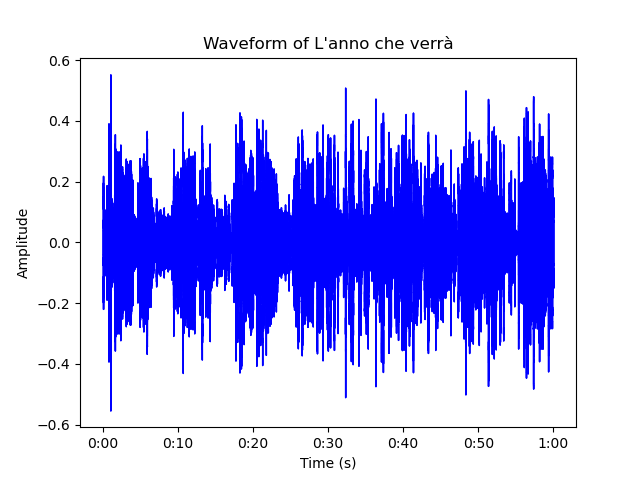
\includegraphics[width=0.9\linewidth]{../Statistical_Sciences_template/figure/Waveform.png}
	\caption{Time-domain waveform of L'anno che verrà from 15s to 75s, showing amplitude variations over time. The horizontal axis represents time in seconds, while the vertical axis shows normalized amplitude. If we reckon the waveform audio signal as a time series, we can intuitively say the process is heteroschedastistic and non-stationary.}
	\label{fig:L'anno che verrà}
\end{figure}
\noindent To address the challenge of non-stationary audio signals, a typical and widely adopted strategy is the application of the Short-Time Fourier Transform (STFT). The fundamental assumption behind STFT is that, although the overall audio signal is non-stationary, it can be considered approximately stationary in short time frames. Within these frames, it is assumed that the spectral characteristics of the signal are approximately constant. In practice, the audio data is segmented into partially overlapping short frames, and for each frame, the Discrete Fourier Transform (DFT) is computed. The steps can be conclude in the following way:\\
\\
\usetikzlibrary{arrows.meta}
\begin{tikzpicture}[->, >=Stealth]
	
	\node[draw, rectangle, minimum width=1.5cm, minimum height=1cm] (A) at (-4.5,0) {Audio Data};
	\node[draw, rectangle, minimum width=1.5cm, minimum height=1cm] (B) at (-1,0) {Pre-emphasis};
	\node[draw, rectangle, minimum width=1.5cm, minimum height=1cm] (C) at (2.5,0) {Framing};
	\node[draw, rectangle, minimum width=1.5cm, minimum height=1cm] (D) at (5.8,0) {Windowing};
	\node[draw, rectangle, minimum width=1.5cm, minimum height=1cm] (E) at (8.5,0) {STFT};	
	
	\draw (A) -> (B);
	\draw (B) -> (C);
	\draw (C) -> (D);
	\draw (D) -> (E);	
\end{tikzpicture}
\\
\section{Mel Scale}

The invention of the Mel scale can be traced back to 1937, as previously mentioned in the introduction. The idea behind it originated from psychological studies in the field of psychology, specifically investigating the non-linear nature of human auditory perception. In their pioneering work, Stevens, Volkmann, and Newman established the foundation of the Mel scale through experimental research demonstrating that the human ear exhibits greater sensitivity to changes in low-frequency sounds and reduced sensitivity at higher frequencies. This means that small changes in low-frequency sounds are more easily perceived than equivalent changes in high-frequency sounds. In the same way it also indicated that the perception of pitch by the human auditory system does not follow a linear relationship with physical frequency. The data from their experiments showed that the relationship between physical frequency (in Hertz) and perceived pitch (in Mels) is non-linear, resembling the shape of an exponential function rather than a straight line. Unfortunately they didn't provide any mathematical formula to describe this phenomenon. Later researchers, building on the foundational experimental data, designed a mathematical model to describe this non-linear relationship more precisely and wildly used today:\\
\begin{equation}
   Mel(f)=2595\log_{10}(1+\frac{f}{700}) \label{Mel Scale}
\end{equation}
where $Mel(f)$ is the Mel scale and $f$ is the frequency. Thus for the convenience of computing, using the base changing formula for logarithm we can get the equivalent one, the formula can be represented in the following way: \\
\begin{equation}
   Mel(f)=1127\ln(1+\frac{f}{700})
\end{equation}
Via these formulas we can transform the nonlinear human pitch perception into a computable linear scale.\\
\\

\section{Mel Frequency Cepstral Coefficients}

The Mel Frequency Cepstral Coefficients (MFCCs) are a widely used feature representation in audio signal processing, particularly effective in tasks such as music genre classification. The computation of MFCCs is fundamentally based on two key components: the Short-Time Fourier Transform (STFT) and the Mel scale. STFT provides a time-frequency representation of the audio signal, capturing its spectral characteristics within short, overlapping frames, while the Mel scale transforms the linear frequency axis into a perceptually motivated scale. The steps are illustrated in the following diagram, which outlines the complete pipeline for MFCC extraction.
\\

\usetikzlibrary{arrows.meta}
\begin{tikzpicture}[->, >=Stealth]

	\node[draw, rectangle, minimum width=1.5cm, minimum height=1cm] (A) at (-4.5,0) {Audio Data};
	\node[draw, rectangle, minimum width=1.5cm, minimum height=1cm] (B) at (0,0) {Audio Preprocessing};
	\node[draw, rectangle, minimum width=1.5cm, minimum height=1cm] (C) at (3.5,0) {STFT};
	\node[draw, rectangle, minimum width=1.5cm, minimum height=1cm] (D) at (6.5,0) {Mel Filterbank};
	\node[draw, rectangle, minimum width=1.5cm, minimum height=1cm] (E) at (9.5,0) {DTC};	
	
	\draw (A) -> (B);
	\draw (B) -> (C);
	\draw (C) -> (D);
	\draw (D) -> (E);	
\end{tikzpicture}
\\
\\
To provide a clearer understanding of the process above for computing MFCCs, it is helpful to break it down step by step.\\
\subsection{Pre-emphasis}
The first step in the MFCC extraction pipeline is pre-emphasis, a preprocessing operation applied to the raw audio signal. The purpose of pre-emphasis is to amplify the high-frequency components of the signal, which are often attenuated during the sound production or transmission process. This step not only improves the spectral balance but also enhances the signal-to-noise ratio for high-frequency elements. Typically, a first-order high-pass filter is employed for pre-emphasis. This filter is simple yet effective and is commonly defined in the time domain by the equation:\\
\begin{equation}
y(t)=x(t)-\alpha x(t-1) \label{pre-emphasis}
\end{equation}

in which $x(t)$ is the input signal, $y(t)$ is the filtered output and  $\alpha$  is the pre-emphasis coefficient, usually chosen in the range of 0.95 to 0.97.In the Z-domain, which is frequently used in digital signal processing for system analysis, the corresponding transfer function of the high-pass filter is:\\
\begin{equation}
H(t)=\frac{Y(z)}{X(x)}=1-\alpha z^{-1}
\end{equation}
where $X(z)=\sum_{t=-\infty}^{\infty}x(t)z^{-t}$ that represents the Z-transform of the input signal and $z$ is complex variable that $z^{-1}$ is the one-step delay operator. The input spectrum multiplied by the transfer function of the high-pass filter is the output spectrum. This spectral filtering emphasizes the higher frequency regions, preparing the signal for subsequent stages. \\
\subsection{Framing and Windowing} \label{subsec:framingwindowing}
The second step is framing and windowing, which prepare the audio signal for localized frequency analysis in the time-frequency domain. In the framing step, the pre-emphasized audio signal is split into short frames that are overlapping with each other, under the assumption that the signal is approximately stationary within each frame. This is a practical simplification, as real-world audio signals——such as speech and music——are always non-stationary, both in the strict and weak statistical sense, as I have illustrated in the first section of this chapter. Hence frames help for a more accurate and localized spectral analysis. For the m-th frame, the signal segment can be defined as:\\
\begin{equation}
y_m[t]=y[t+m\times h], \qquad 0\leq t<L \label{framing}
\end{equation}
where $y(t)$ is the pre-emphasized signal from \eqref{pre-emphasis}, $L$ is the frame length and $h$ is the hop size which determines the step between consecutive frames and controls the degree of overlap.
Following framing, a window function is applied to each frame to reduce spectral leakage—a phenomenon that arises due to the finite length of frames, which can introduce discontinuities at the boundaries and distort the spectral representation. To mitigate this, each frame is multiplied element-wise by a tapering function that smooths the edges. Two commonly used window functions are the Hamming window and the Hann window, defined respectively as:\\
  Hamming:
  \begin{equation}
  w[t]=0.54-0.46\cos(\frac{2\pi n}{L-1}) \label{Hamming}
  \end{equation}
  Hann:
  \begin{equation}
  w[t]=0.5-0.5\cos(\frac{2\pi n}{L-1}) \label{Hann}
  \end{equation}
The windowed frame is then computed by multiplying the framed signal by the window function:\\
\begin{equation}
	y_{win}[t]=y_m[t]\times w[t] \label{windowing}
\end{equation}
\subsection{Short-Time Fourier Transformation}
The third step is to perform Fourier transformation on each frame of signal. This transformation converts the time-domain signal into its frequency-domain representation, yielding a complex-valued spectrum for each frame, that is $X_m[k]$ where $k$ is the frequency bin index. The discrete Fourier Transform (DFT) of a windowed signal frame can be computed as follows:\\
\begin{equation}
X_m[k]=\sum_{t=0}^{L-1}y_{win}[t]\times e{\frac{-2\pi kti}{N}} \label{DFT}
\end{equation}
where i represents the imaginary unit satisfying $i^2=-1$, $N$ is DFT size and k is the frequency bin index.\\
\\
The results of $X_m[k]$ are complex numbers representing the magnitude and phase of the frequency component at bin $k$ for frame $m$. However, for most MFCC applications, only the magnitude or power spectrum are used, discarding the phase information. To obtain the amplitude spectrum, we compute the modulus of the complex DFT coefficients: \\
\begin{equation}
|X_m[k]|=\sqrt{Real(X_m[k])^2+Imag(X_m[k])^2}
\end{equation} 
Alternatively, the power spectrum can be obtained by squaring the amplitude:
\begin{equation}
|X_m[k]|^2=Real(X_m[k])^2+Imag(X_m[k])^2
\end{equation}
This step provides a frequency-based representation of each frame that captures how energy is distributed across frequency bands. The $k\times m$ matrix of power spectra (more popular) is then passed to the Mel filter bank in the next step to simulate the human auditory system’s nonlinear frequency resolution.\\
\subsection{Mel Filter Bank}
Hence the fourth step is the construction of the Mel filter bank, which plays a key role in modeling the human auditory system’s nonlinear perception of frequency. The Mel filter bank is composed of a set of overlapping triangular filters that are spaced linearly on the Mel scale but non-linearly on the Hertz (Hz) scale.\\
\\
The first consideration in designing the Mel filter bank is to determine the frequency range. Typically, this range should cover the entire audible frequency spectrum for humans, which is approximately 20 Hz to 20,000 Hz. However, in practice, the upper bound is often constrained by the Nyquist frequency, which is half the sampling rate of the audio signal. For example, if the sampling rate is 22050 Hz, the Mel filter bank will be designed from 0 Hz to 11025 Hz.\\
\\
Once the frequency range in Hz is determined, the next step is to map these boundaries to the Mel scale using \eqref{Mel Scale}. Specifically, we compute:
\begin{equation}
Mel_{min}=Mel(0), \qquad  Mel_{max}=Mel(f_{max})
\end{equation}
where $f_max=\frac{sampling rate}{2}$ mentioned above.\\
\\
Next, we decide on the number of filters, denoted by $\nu$, which determines the frequency resolution in the perceptual domain. Based on this, we partition the Mel scale uniformly into $\nu+2$ points, corresponding to the lower edge, center, and upper edge frequencies of each triangular filter. These center Mel frequencies are spaced across the interval $[Mel_{min}, Mel_{max}]$. After obtaining these center points on Mel scale, we can convert them back to the form of Hertz using the inverse formula of \eqref{Mel Scale}, that is: \\
\begin{equation}
f=700\times (10^{\frac{Mel}{2595}}-1)
\end{equation}\\
Once the center frequencies have been determined and mapped back to the Hertz domain, the next step is to construct the triangular Mel filters.These filters are designed to mimic the frequency resolution of the human ear by emphasizing specific frequency bands and smoothing transitions between adjacent bands. As previously noted, the filters are overlapping and each has a triangular shape with values ranging from 0 to 1. For example, the $\kappa$-th filter denoted as $H_{\kappa}(f)$ is defined over the interval $[f_{\kappa-1},f_{\kappa+1}]$ where $f_{\kappa-1}$, $f_{\kappa}$ and $f_{\kappa+1}$ are the lower boundary, center frequency, and upper boundary of the filter in Hertz domain respectively. The filter starts with a value of 0 at $f_{\kappa-1}$, increases linearly to a peak value of 1 at the center point $f_{\kappa}$, and then decreases linearly back to 0 at $f_{\kappa+1}$.  Mathematically, this can be expressed as:\\
\begin{equation}
H_{\kappa}(f)=
\begin{cases}
	0  & f<f_{\kappa-1}\\
	\frac{f-f_{\kappa-1}}{f_{\kappa}-f_{\kappa-1}}  & f_{\kappa-1}\leq f<f_{\kappa} \\
	\frac{f_{\kappa+1}-f}{f_{\kappa+1}-f_{\kappa}}  & f_{\kappa}\leq f<f_{\kappa+1} \\
	0  & f \geq f_{\kappa+1}
\end{cases}	
\end{equation}
Each filter effectively weights the STFT spectrum based on how close a frequency component is to the filter's center frequency. This construction ensures that each frequency bin contributes to multiple filters, allowing the system to capture smooth transitions and localized energy in neighboring frequency bands. The overlapping nature of the filters also reflects the way human auditory perception blends adjacent frequencies rather than treating them as completely distinct.\\
\\
Figure~\ref{fig:Mel filters} illustrates an example of a Mel filter bank spanning the frequency range from 0 to 11025 Hz, constructed with 10 triangular filters. In the figure, the red triangle represents the $\kappa$-th filter $H_{\kappa}(f)$, while the blue and green triangles correspond to the adjacent filters $H_{\kappa-1}(f)$ and $H_{\kappa+1}(f)$ respectively. As shown, the filters are overlapping, with each one peaking at its center frequency and tapering linearly to zero at the boundaries shared with neighboring filters. The widths of the triangles vary, reflecting the non-linear spacing of Mel-scale frequencies when mapped back to the linear Hertz scale. But in practice, especially in analysis of music we will design more Mel filters for weighting the results of the STFT matrix.\\
\begin{figure}
	\centering
	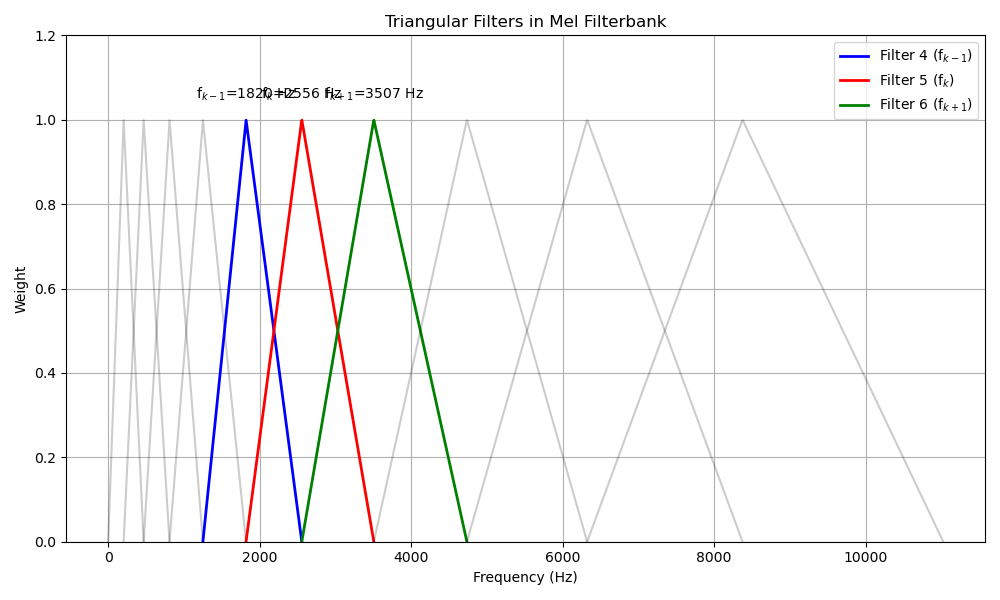
\includegraphics[width=0.9\linewidth]{../Statistical_Sciences_template/figure/example of Mel filters.png}
	\caption{}
	\label{fig:Mel filters}
\end{figure}\\
After constructing the Mel filter bank, the next step is to compute the Mel-scale energy coefficients, which represent the energy content of the signal in perceptually motivated frequency bands. This step effectively transforms the detailed frequency representation obtained from the power spectrum into a compact and interpretable form aligned with the Mel scale. The computation consists of two primary stages. First, the power spectrum $|X_m[k](f)|^2$ of each frame (as derived from the STFT) is weighted by the Mel filter bank. For each Mel filter $H_{\kappa}$, the power spectrum is multiplied point-wise by the filter’s response across frequencies.Next, the weighted values are summed to obtain the total energy within each Mel frequency band. This aggregation yields the Mel energy coefficient for the $\kappa$-th filter, which can be expressed mathematically as:\\
\begin{equation}
Mel_{\kappa}=\sum_{f} |X_m[k](f)|^2 \times H_{\kappa}(f)
\end{equation}
where $Mel_{\kappa}$ is the energy in the $\kappa$-th Mel band for the m-th frame.\\ 
\\
The final step of this part is to do logarithm compression for the Mel scale energy coefficients. The purpose of this operation is to compress the dynamic range of Mel energies enhancing low-amplitude components while taming high-amplitude peaks. In this compression we must choose a small constant denoted as $\epsilon>0$ to avoid computing $\log(0)$ and then compute the log-Mel spectrum within $\log(Mel_{\kappa}+\epsilon)$. Finally denoting the number of Mel scale energy coefficients as $\nu_{mel}$, we can get a $\nu_{mel} \times m$ matrix.\\
\subsection{Discrete Cosine Transform}
The final stage in computing Mel Frequency Cepstral Coefficients (MFCCs) is to apply the Discrete Cosine Transform (DCT) to the log-transformed Mel energy coefficients. This step serves two primary purposes: first, it decorrelates the log-Mel energies, making the resulting features approximately orthogonal and hence more suitable for statistical modeling; second, it helps to separate the spectral envelope (which carries information about the timbre of the sound) from the excitation signal (which often corresponds to pitch or voiced/unvoiced characteristics). More specifically, the DCT Type-II is typically applied, which transforms the logarithmic Mel spectrum into the cepstral domain. The transformation is defined as follows:\\
\begin{equation}
	MFCC_n=\sum_{\kappa=1}^{\nu_{mel}}[\log(Mel_{\kappa})\times \cos(\frac{n(\kappa-0.5)\pi}{\nu_{mel}})]
\end{equation}
where $n$ is the index of the cepstral coefficients and $MFCC_n$ is the $n$-th Mel frequency cepstral coefficient. Typically $n$ ranges from 0 to 12 or 13, but in some situations more will be taken. Finally we got a $n \times m$ matrix.\\
\\
By concentrating most of the signal energy in the lower-order coefficients, the DCT facilitates dimensionality reduction and helps isolate perceptually significant information. In practice, only the first few MFCCs are retained, as they capture the most relevant features of the audio signal's spectral shape, while higher-order coefficients are often discarded or used selectively depending on the application.\\
\subsection{An Example of MFCC}

To illustrate the process concretely, I also take L'anno che verrà as an example. The audio file used in this example has a standard sampling rate of 44.1 kHz, as mentioned in the first section of this chapter. For the purposes of analysis, I selected a 60-second excerpt beginning at the 15-second mark. In preparing the signal for time-frequency analysis, I chose a window size (also referred to as the frame length) of 1024 samples. This corresponds to a segment of the audio that spans:\\
$$
	\frac{1024}{44100}\approx0.0232 \ \text{seconds} \qquad \text{(or approximately 23 milliseconds)}
$$
It is worth noting that this duration is significantly shorter than a full second, as one-second windows typically capture too much variation in dynamic audio signals, making it difficult to assume any form of stationarity within them.\\
To allow for continuity and smoother temporal analysis, a hop size of 256 samples was used, which is exactly one-quarter of the window size. This means that each analysis window overlaps 0.75 with the next. The hop duration in time can be calculated as:\\
$$
	\frac{256}{44100}\approx0.0058 \ \text{seconds} \qquad \text{(or approximately 5.8 milliseconds)}
$$
After framing and windowing, MFCCs are computed per frame. For this example, I selected the standard 13 MFCCs ($n=13$) per frame, which is a commonly used configuration in audio analysis as it strikes a balance between capturing relevant spectral features and avoiding redundancy. The output of the MFCC process is a matrix of size $n \times m$, where $m$ represents the total number of frames computed for the audio segment.\\
\\
The total number of frames $m$ is calculated by the following formula
\begin{equation}
	number\textunderscore of\textunderscore frames=\lceil \frac{sample\textunderscore rate \times duration-frame \textunderscore length}{hop\textunderscore length}+1 \rceil
	\label{windownumber}
\end{equation}\\
In our situation:
\begin{itemize}
	\item $\text{sample\_rate} = 44100$,
	\item $\text{duration} = 60$ seconds,
	\item $\text{frame\_length} = 1024$, and
	\item $\text{hop\_length} = 256$.
\end{itemize}
Hence substitute the values we can get:\\
$$
number\textunderscore of\textunderscore frames=\lceil \frac{44100*60-1024}{256}+1\rceil=10333
$$\\
Therefore, the resulting MFCC matrix has dimensions $13\times 10333$.\\
\\
The following figure \ref{fig:MFCC Example} is the MFCC spectogram of the piece of music. For the $y$ axis it is divided into 13 intervals that corresponds to the 13 MFCCs. Thus the $x$ axis various over time from 0s to 60s, hence the figure illustrate how energy distribution during the time. For example, the high-order MFCCs are almost uniformly distributed from 30s to 40s. It is possible that some instruments are playing continuously, making the energy change less obvious, while there is a significant energy changes from 25s to 30s. \\
\\
\begin{figure}
	\centering
	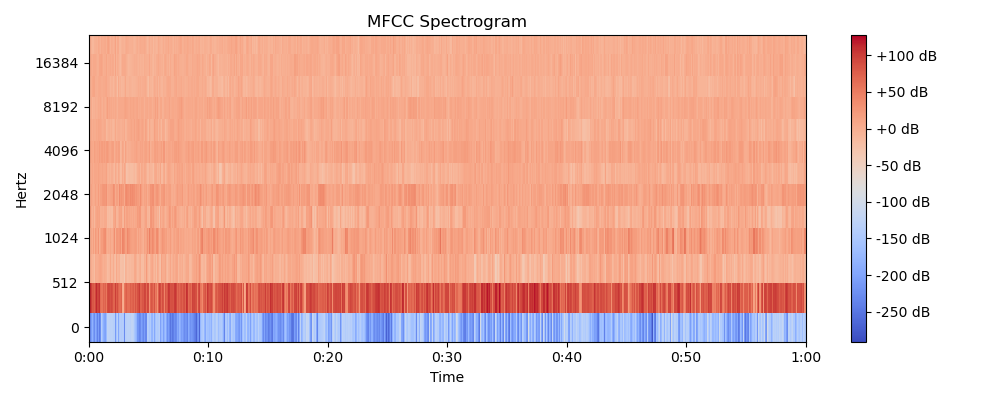
\includegraphics[width=0.9\linewidth]{../Statistical_Sciences_template/figure/MFCC Example.png}
	\caption{}
	\label{fig:MFCC Example}
\end{figure}\\
The first few MFCCs (such as the 1st to 3rd dimensions) mainly capture the characteristics of the vocal tract (low-frequency cepstrum components). These coefficients reflect the spectral envelope characteristics of the sound, especially the resonance peak structure that is closely related to the shape of the vocal tract. Since the vocal tract changes relatively slowly (such as the movement of the vocal organs takes a certain amount of time), as shown in figure \ref{fig:Low MFCCs}, these low MFCCs appear as curves in the time domain that do not change particularly drastically, but the difference is significant.\\
\\
\begin{figure}[h!]
	\centering
	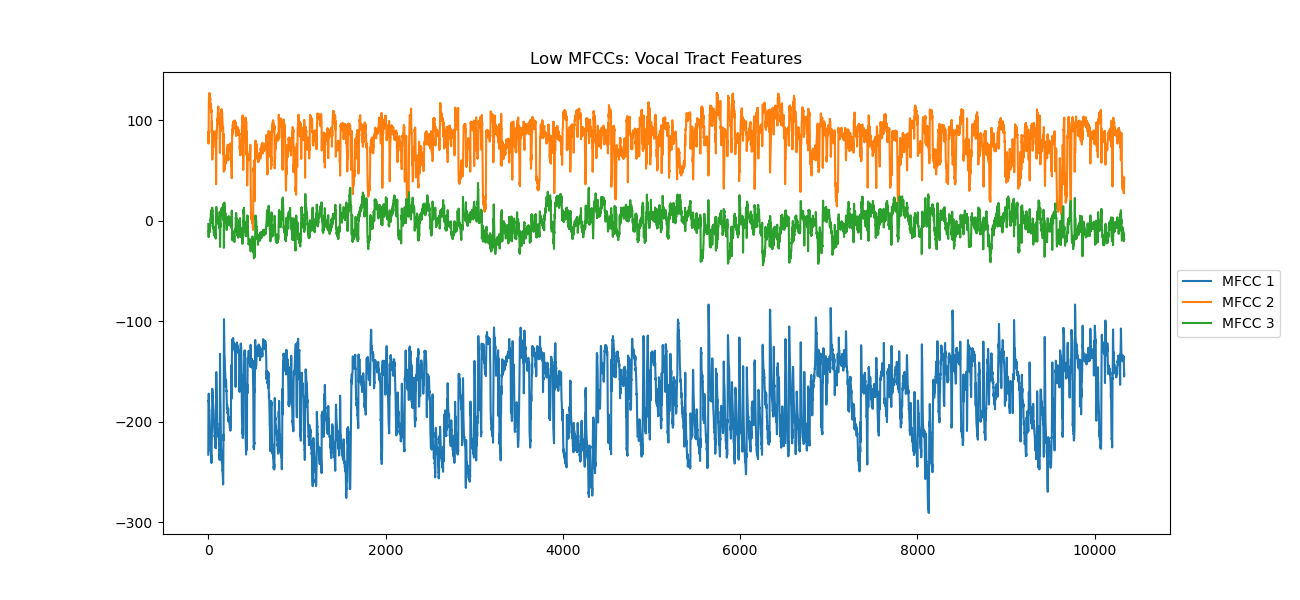
\includegraphics[width=0.9\linewidth]{../Statistical_Sciences_template/figure/Low MFCCs.png}
	\caption{}
	\label{fig:Low MFCCs}
\end{figure}\\
However, high-order MFCCs (such as the 11th-13th dimension and above) mainly reflect the detailed characteristics of the excitation source (high-frequency cepstrum components). These coefficients record the finer time-varying characteristics of the sound signal. Since the characteristics of the excitation source (such as the fundamental frequency generated by the vibration of the vocal cords or the random noise of the unvoiced sound) often have rapidly changing transient characteristics, they are manifested as violent fluctuations in the high-frequency coefficient curve in the MFCC spectrogram as shown in figure \ref{fig:High MFCCs}. This fluctuation pattern is directly related to the excitation characteristics of the sound. It is worth noting that high-order MFCC coefficients often show a high degree of similarity. This is because in these cases, the characteristics of the excitation source (such as the vocal cord vibration mode or the noise characteristics) remain relatively constant, and the changes mainly occur in the vocal tract characteristics.\\
\begin{figure}[h!]
	\centering
	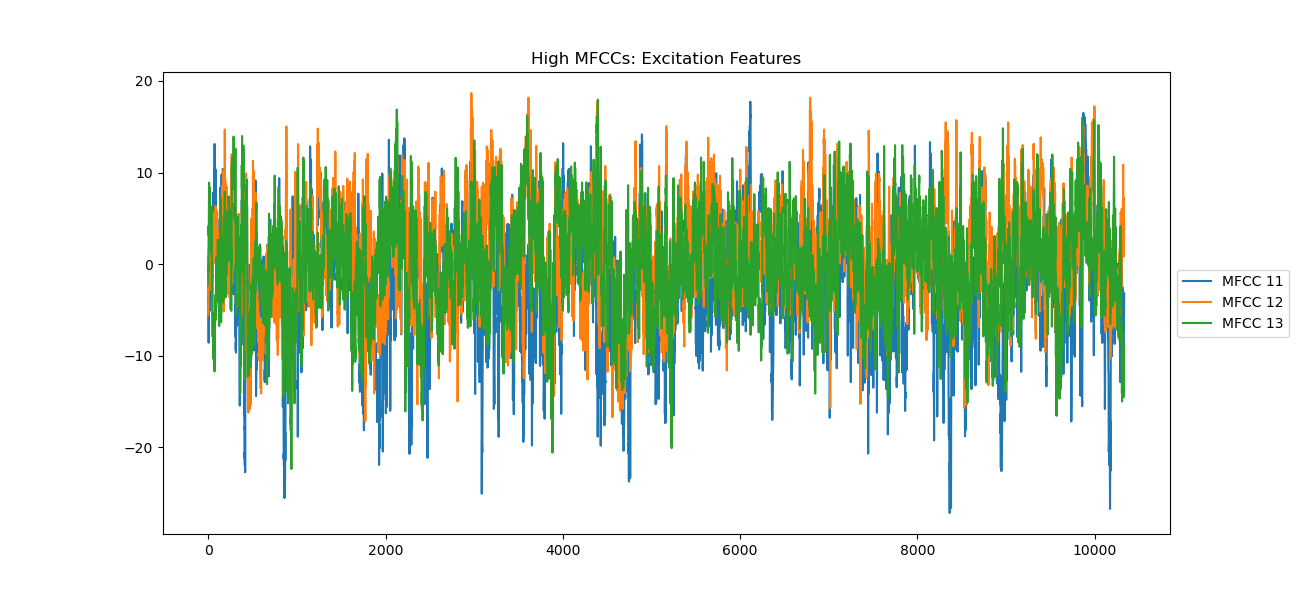
\includegraphics[width=0.9\linewidth]{../Statistical_Sciences_template/figure/High MFCCs.png}
	\caption{}
	\label{fig:High MFCCs}
\end{figure}\\

\section{Shapelet Tree-Based Classification}

This algorithm is inspired by the foundational work of L. Ye and E. Keogh (2009), which introduced a novel approach for time series classification based on the concept of shapelets. A shapelet is defined as a subsequence of a time series that is maximally representative of a particular class. In other words, a shapelet captures a discriminative pattern or local structure that tends to appear in time series belonging to one class but not in others. The primary objective of the algorithm is to identify the most informative shapelet——i.e. the one that best separates the classes. This is typically achieved by evaluating candidate subsequences based on their ability to split the dataset according to a distance threshold, using measures such as information gain to quantify the separation.\\
\\
Once the optimal shapelet has been discovered, it can be used to transform the time series into a new feature space where each instance is represented by its distance to the shapelet(s). This transformation enables the application of traditional classification techniques such as decision trees, as the complex temporal data are now reduced to a more tractable feature-based representation. The shapelet-based approach provides both interpretability, as the identified shapelets can be visualized and interpreted as the key patterns driving the classification. This makes the algorithm particularly valuable in domains where understanding the decision process is important.\\
\subsection{Key Definitions}
Before delving into the details of the algorithm, it is essential to introduce several key definitions that form the theoretical foundation for understanding the overall process. These definitions help clarify the notions of distance between time series and provide a framework for comparing sequences of potentially different lengths.
\begin{definition}[Distance of time series with the same length]%
Let $Dist(T_1,T_2)$ denote the distance between two discrete time series $T_1$ and $T_2$, where $T_1$ and $T_2$ are two discrete time series who may have the same length. A valid distance function must satisfy the following properties:\\
1. Symmetry: $Dist(T_1,T_2)=Dist(T_2,T_1)$ and \\
2. Non-negativity: $Dist(T_1,T_2) \geq 0$. 
\end{definition}%
\noindent For example, if we compute the Euclidean distance between $T_1$ and $T_2$, the formula follows:
$$
Dist(T_1,T_2)=(\sum_i(T_{1i}-T_{2i})^2)^{\frac{1}{2}}
$$
Alternatively, the Manhattan distance can be used:\\
$$
Dist(T_1,T_2)=\sum_i|T_{1i}-T_{2i}|
$$
In practical applications, it is more common to encounter the cases that two time series do not have equal lengths, i.e., $length(T_1^*) \neq length(T_2^*)$. Without lose generality, we can assume $length(T_1^*)\geq length(T_2^*)$. In such cases, we consider the distance between the two time series is based on the best matching subsequence of the longer series $T_1^*$. Hence the distance between $T_1^*$ and $T_2^*$ can be define as:

\begin{definition}[Distance of time series]\label{def:Dist}%
$Dist(T_1^*,T_2^*)=\min_{S\subseteq T_1^*}(Dist(S,T_2^*))$ where $S$ is a subsequence of $T_1^*$ having the same length as $T_2^*$ 
\end{definition}%
\noindent Another key concept in this algorithm is the notion of a shapelet, which can be described as follows:
\begin{definition}[Shapelet]\label{def:shapelet}%
	Give a labeled time series dataset $\boldsymbol{D}$ which contains two classes of observations, denoted as $A$ and $B$, shapelet($\boldsymbol{D}$) is defined as a subsquence of a time series within $\boldsymbol{D}$ that best separates the observations according to their class labels.
\end{definition}%
\noindent In other words, a shapelet is a short, discriminative segment of a time series that captures distinctive features associated with one class and is absent or significantly different in the other. The fundamental idea behind using shapelets is that certain local patterns, rather than the entire time series, can be highly informative for classification. Once a candidate shapelet has been extracted, the algorithm evaluates its usefulness by assessing how well it partitions the dataset based on similarity to the shapelet. Moreover to evaluate how well a given subsequence (i.e., a shapelet candidate) can partition the dataset according to the class labels, this algorithm uses information gain (IG) as the primary quality metric. Information gain measures the reduction in uncertainty (entropy) about class membership after the dataset has been split based on the shapelet. It can be calculated as:\\
\begin{equation}
	IG=I(\boldsymbol{D})-f(\boldsymbol{D_1})\times I(\boldsymbol{D_1})-f(\boldsymbol{D_2})\times I(\boldsymbol{D_2})
	\label{IG}
\end{equation}
where $I(\boldsymbol{D})$ denotes the entropy of the original dataset $\boldsymbol{D}$, while $I(\boldsymbol{D_1})$ and $I(\boldsymbol{D_2})$ are the entropies of the two subsets resulting from a split based on a candidate shapelet. ,$f(D_i) \forall i=1,2$ represent the proportion of observations of $D_1$ and $D_2$ in $D$ respectively.\\
\\
By using formula \eqref{IG}, we can compute the information gain of each split datasets $D_1$ and $D_2$, and we can choose the best sequence that gives the largest information gain as the shapelet. Hence only one problem is remained that is how the shapelet can classify the time series datasets and find the best split point that corresponds to the shapelet. Here follows another definition of vital importance:
\begin{definition}[Optimal Split Point]
Given a time series dataset $\boldsymbol{D}$ consisting of two classes $A$ and $B$, for a shapelet candidate $S$, we can choose a distance threshold $d_{th}$ splitting $\boldsymbol{D}$ into two subsets $\boldsymbol{D_1}$ and $\boldsymbol{D_2}$ whose intersection is empty, i.e. $\boldsymbol{D_1} \cap \boldsymbol{D_2}=\emptyset$, such that $\{T_i, Dist(T_i,s)\leq d_{th} \forall T_i \in \boldsymbol{D} \}$ are assigned to one class and $\{T_i, Dist(T_i,s) > d_{th} \forall T_i \in \boldsymbol{D} \}$ are assigned to the other class. Thus the optimal split point (OSP) is the threshold that 
$$
	IG(S, d_{OSP}) \geq IG(S, d_{th})
$$
In other words, the OSP is the threshold that:\\
$$
	d_{OSP}=\arg \max_{d_{th}} IG (S,d_{th})
$$
\label{def:OSP}
\end{definition}

\begin{figure}[h!]
	\centering
	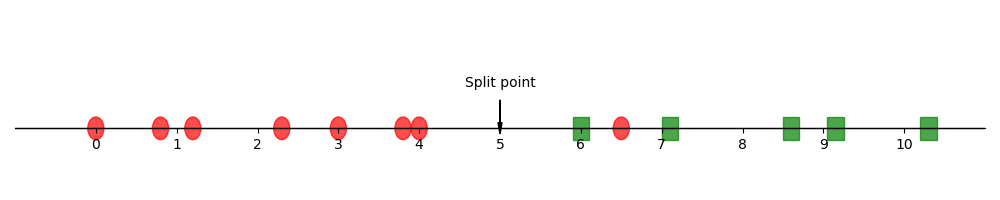
\includegraphics[width=0.9\linewidth]{../Statistical_Sciences_template/figure/OSP.png}
	\caption{There are 13 observations in the dataset, they are shown via the distances of candidate shapelet $S$, and the shapes corresponds to different labels. The optimal split point is the center point between the 7th sorted observation and the 8th sorted observation}
	\label{fig:OSP}
\end{figure}

\noindent To illustrate the concept of the optimal split point, we can refer to the Figure \ref{fig:OSP}. The process begins by computing the distance between a candidate shapelet $S$ that is a subsequence of one time series from $\boldsymbol{D}$ and all the times series in dataset $D$. If the dataset $D$ contains $n$ observations we will obtain $n$ distance values. Because each time series in the dataset is labeled, we can sort the distances in ascending order and associate them with their corresponding class labels. Using this sorted list, we iterate over all possible split points between consecutive distances and calculate the entropy of the resulting subsets for each threshold. The information gain is computed for each potential split using Equation \eqref{IG}, and the threshold that results in the highest information gain is selected as the optimal split point.\\
\\
This approach allows the algorithm to determine both the most discriminative shapelet and the decision boundary (distance threshold) that best separates the classes, forming the basis for subsequent classification of new time series based on their similarity to the learned shapelet.\\
\\
\subsection{Achieve of the Shapelet Algorithm}\label{sec:algo}

To implement the shapelet-based classification algorithm, the first and most crucial step is to generate all possible shapelet candidates $S$ from the given time series dataset $D$ referring to Definition \ref{def:shapelet}. In practice, shapelet candidates are formed by extracting all possible contiguous subsequences from the time series instances in $D$. Hence the generating step can be achieve as follows:\\
\begin{algorithm}[h!]
	\caption{Candidate Shapelets Generating}
	\begin{algorithmic}[1]{
		\Procedure{generate\ candidates}{$\mathtt{Time\ Series}\ T$, $MINLEN$, $MAXLEN$}
		\State $pool \gets \emptyset$
		\State $l \gets MAXLEN$
		\While{$l \geq MINLEN$}{
			\For{$i \gets 1$ \textbf{to} $\mathrm{len}(T) - l$}
			\State \textbf{EXTRACT subsequence from T starting at i with length l} 
			\State \textbf{ADD subsequence to pool} 
			\EndFor
		}
		\State $l \gets l - 1$
		\EndWhile
		\EndProcedure
	}
	\end{algorithmic}
	\label{al:CandidateGenerate}
\end{algorithm}
\\
As mentioned above, this function is designed to generate the complete set of consecutive subsequence candidates from a given time series sequence $T$ where the lengths of the subsequences range from a specified minimum length $MINLEN$ to a maximum length $MAXLEN$. The goal is to produce all possible contiguous segments of $T$ that fall within this length interval, which will later be evaluated for their usefulness as shapelets.\\
\\
The implementation follows a nested loop structure:
\begin{quote}
1. The outer loop iterates over the possible subsequence lengths l, starting from $MAXLEN$ and decrementing down to $MINLEN$. This ordering ensures that longer subsequences are generated and added to the pool before the shorter ones.\\
\\
2. For each fixed length $l$, the inner loop performs a sliding window operation across the sequence $T$. It moves a window of length 
$l$ one step at a time (i.e., with a stride of 1), starting at every valid index $i$ such that the subsequence $T[i:i+1]$ emains within bounds.
\end{quote}
Each generated subsequence is stored in the candidate pool. This format facilitates efficient indexing and retrieval in later stages of the algorithm, particularly when computing distances and information gain. The final output of the function is a list containing all valid subsequences from T whose lengths fall within the defined range. The resulting pool is ordered from longest to shortest subsequences, reflecting the traversal logic described above.\\
\\
After obtaining the complete set of candidate subsequences—also known as shapelet candidates—the next critical step is to compute the distances between each shapelet and all time series in the dataset referring to Definition \ref{def:Dist}. This involves sliding each shapelet across every time series and calculating the minimum distance between the shapelet and the most similar subsequence within each series. The algorithm can be achieve as follows:\\
\begin{algorithm}[H]
	\caption{Time Series Distance}
	\begin{algorithmic}[1]{
			\Procedure{subsequence\ dist}{$\mathtt{Time\ Series}\ T$, $\mathtt{Time\ Series}\ S$, $metric$}
			\State $len \textunderscore T \gets \mathtt{LENGTH\ of}\ T$
			\State $len \textunderscore S \gets \mathtt{LENGTH\ of}\ S$
			\State $min \textunderscore dist \gets +\infty$
			\For{$i \gets 1$ \textbf{to} $(len \textunderscore T - len \textunderscore S)$}
			\State $window \gets T[i:\ i + len \textunderscore S]$
			\State $dist \gets Dist(window,S)$ 
			\If {$dist< min \textunderscore dist$}
			\State $min \textunderscore dist \gets dist$ 
			\EndIf
			\EndFor
			\EndProcedure
		}
	\end{algorithmic}
	\label{al:DIST}
\end{algorithm}

\noindent This function calculates the distance of the subsequence most similar to the target sequence S in the sequence T, and controls the measurement methods of distance through the variable metric, such as two measurements: Euclidean and Manhattan distance (L1). Iterate through the sliding window all subsequences of length $len(S)$ in $T$. For each window, calculate its distance from $S$ according to the specified metric: if it is the Euclidean distance, calculate the sum of the squared difference; if it is the Manhattan distance, calculate the sum of the absolute difference. Finally, the minimum value of all window distances is returned.\\
\\
Next, using the distances computed in the previous step, the algorithm proceeds to identify the optimal split point. As outlined in the previous section and formally defined in Definition \ref{def:OSP}, this step is crucial for evaluating how effectively a shapelet can separate the time series into distinct classes. The process begins by sorting the computed distances between a candidate shapelet and all time series in ascending order. This sorted list enables us to systematically examine potential thresholds for splitting the dataset. Once the distances are sorted, a distance-based histogram is constructed, where each bin corresponds to a range of distances, and each time series is assigned a class label. The algorithm goes as follows:\\
\begin{algorithm}[H]
	\caption{Check Candidate}
	\begin{algorithmic}[1]{
			\Procedure{checkcandidate}{$\boldsymbol{D}$, $S$, $original\textunderscore label$}
			\State $object_histogram \gets \emptyset$
			\For{$\mathtt{EACH}\ T$ \textbf{in} $\mathtt{Dataset}\ \boldsymbol{D}$}
			\State $dist \gets SUBSEQUENCEDIST(T,S)$
			\State \textbf{ADD dist to} $object_histogram$
			\EndFor
			\State \textbf{RETURN CalculateInformationGain}$(object\textunderscore histogram, original\textunderscore label)$
			\EndProcedure
		}
	\end{algorithmic}
	\label{al:checkcandidate}
\end{algorithm}
\noindent The purpose of this function is threefold: (1) calculate the minimum distance between the candidate shapelet $S$ and every sequence in the dataset $D$ using a specified distance metric, (2) compile a histogram of these distances, and (3) compute the information gain associated with the best possible split based on these distances.\\
\\
The specific process unfolds as follows:
\begin{quote}
1. Iterate over each time series $T$ in the dataset $\boldsymbol{D}$. For each sequence, the function invokes SUBSEQUENCEDIST referring the Algorithm \ref{al:DIST}, which calculates the distance between $S$ and $T$, using the chosen metric (e.g., Euclidean or Manhattan distance). This results in a single scalar value representing how closely $T$ matches $S$.\\
2. Each computed distance is then stored in a list called object\textunderscore histogram, which contains the distance values. \\
3. The histogram and original class labels are passed to the CalculateInformationGain function.
\end{quote}

\noindent But in the Algorithm \ref{al:checkcandidate} there is another function to be used, that is CalculateInformationGain, which aims at finding the optimal split of the input shapelet, calculating the information gain and split the time series dataset $\boldsymbol{D}$ into two $\boldsymbol{D_1}$ and $\boldsymbol{D_2}$. To complete this function the algorithm follows:
\begin{algorithm}[H]
	\caption{Calculate Information Gain}
	\begin{algorithmic}[1]{
			\Procedure{CalculateInformationGain}{$object\textunderscore histogram$, $original\textunderscore label$}
			\State $key \gets \mathtt{Empty\ dictionary}$
			\State $\boldsymbol{D_1} \gets \emptyset$
			\State $\boldsymbol{D_2} \gets \emptyset$
			\State $split\textunderscore 	point \gets$ \textbf{OptimalSplitPoint}($object\textunderscore histogram$, $original\textunderscore label$)
			\For{$d$ \textbf{in} $object\textunderscore histogram$}
			\If{$d \leq split_point$}
			\State $\boldsymbol{D_1} \gets \boldsymbol{D_1} \bigcup d$ 
			\Else $\boldsymbol{D_2} \gets \boldsymbol{D_2} \bigcup d$ 
			\EndIf
			\EndFor	
			\State $Entropy_{\boldsymbol{D}} \gets ENTROPY(\boldsymbol{D})$
			\State $Entropy_{\boldsymbol{D_1}} \gets ENTROPY(\boldsymbol{D_1})$
			\State $Entropy_{\boldsymbol{D_2}} \gets ENTROPY(\boldsymbol{D_2})$
			\State $Proportion_{\boldsymbol{D_1}} \gets PROPORTION(\boldsymbol{D_1})$
			\State $Proportion_{\boldsymbol{D_2}} \gets PROPORTION(\boldsymbol{D_2})$
			\State $IG \gets Entropy_{\boldsymbol{D}}-(Proportion_{\boldsymbol{D_1}} \times Entropy_{\boldsymbol{D_1}}+Proportion_{\boldsymbol{D_2}} \times Entropy_{\boldsymbol{D_2}})$
			\State \textbf{Store} $split\textunderscore point$, $IG$, $\boldsymbol{D_1}$, $\boldsymbol{D_2}$ \textbf{in} $key$
			\State \textbf{Return} $key$
			\EndProcedure
		}
	\end{algorithmic}
	\label{al:CIG}
\end{algorithm}

\noindent This function is responsible for computing the information gain associated with a candidate shapelet by analyzing the distances between that shapelet and each time series in the dataset. Its primary purpose is to identify the best split point—a threshold distance value—that can divide the dataset into two disjoint subsets in a way that maximally separates the two classes. This split enables the algorithm to classify the time series based on their similarity to the shapelet.\\
\\
The procedure begins by receiving a list of distance values between the candidate shapelet and all instances in the dataset, along with their corresponding class labels. The function then systematically examines different possible thresholds (split points) along the range of distance values. For each potential threshold, the dataset is partitioned into two groups:
\begin{itemize}
	\item One group contains all time series with distances less than or equal to the threshold.
	\item The other group contains those with distances greater than the threshold.
\end{itemize}
For every such partition, the function computes the entropy of the original dataset and the entropies of the two resulting subsets. These values are used to calculate the information gain, which measures how effectively the current split reduces uncertainty (i.e., class impurity) in the dataset. The function evaluates all possible split points and selects the one that produces the maximum information gain. This optimal split point (OSP) is considered the threshold at which the shapelet most effectively divides the dataset into more homogeneous class-based groups.\\
\\
Finally, the function returns a data structure that includes: 
\begin{itemize}
	\item The best split point (threshold),
	\item The maximum information gain associated with this split,
	\item And the resulting partitioned subsets or metadata describing the split.
\end{itemize}
This process is a key component in shapelet-based classification algorithms, as it allows the system to identify not only which subsequences (shapelets) are most representative of class distinctions but also how to use them to effectively divide and classify the dataset.\\
\\
All of the procedures described above are designed to achieve a specific goal: to divide the dataset into two subsets using a SINGLE shapelet based on the OSP that maximizes information gain. However as outlined in Algorithm \ref{al:CandidateGenerate}, the number of possible shapelet candidates can be very large, since they are generated by extracting valid subsequences from all time series in the dataset within a given length range. As a result a critical next step is to systematically evaluate all these candidates to determine which one is the most effective. In other words, the task now becomes identifying the best shapelet——the one that produces the maximum information gain when used to split the dataset. This shapelet is considered the most discriminative, as it best captures the structural difference between the classes and serves as the strongest indicator for classification. The Algorithm \ref{al:bestshapelet} follows:
 \begin{algorithm}[H]
 	\caption{Find Best Shapelet}
 	\begin{algorithmic}[1]{
 			\Procedure{FindBestShapelet}{$\boldsymbol{D}$, $MAXLEN$, $MINLEN$, $original\textunderscore label$, $metric$}
 			\State $bsf \textunderscore gain \gets 0$
 			\State $bsf \textunderscore shapelet \gets \emptyset$
 			\State $split \textunderscore point \gets 0$
 			\For{$T$ \textbf{in} $\boldsymbol{D}$}
 				\State $candidates \gets generate\textunderscore candidates(T, MAXLEN, MINLEN)$
 				\State \textbf{Sort} $candidates$
 				\For{$S$ \textbf{in} $candidates$}
 					\State $check \gets checkcandidate(\boldsymbol{D}, S, original\textunderscore label, metric)$
 					\State $gain \gets check["IG"]$
 					\If{$gain > bsf \textunderscore gain $}
 						\State $bsf \textunderscore gain \gets gain$
 						\State $bsf \textunderscore shapelet \gets S$
 						\State $split \textunderscore point \gets check["split\textunderscore point"]$
 						\State $\boldsymbol{D_1} \gets check["D1"]$
 						\State $\boldsymbol{D_2} \gets check["D2"]$
 					\EndIf
 				\EndFor
 			\EndFor	
 			\State \textbf{Return a Dictionary Containing} $bsf \textunderscore gain$, $bsf \textunderscore shapelet$, $split \textunderscore point$, $\boldsymbol{D_1}$, $\boldsymbol{D_2}$
 			\EndProcedure
 		}
	\end{algorithmic}
	\label{al:bestshapelet}
\end{algorithm}
\noindent The function begins by initializing variables to keep track of the best information gain found so far, as well as the corresponding optimal shapelet and relevant statistics. It then iterates over each time series instance in the dataset. For each instance, the function generates candidate subsequences spanning all valid lengths within a predefined range. These candidates are sorted in descending order of length, which can help improve computational efficiency by exploring longer, potentially more informative shapelets first. Next, the function evaluates the discriminative power of each candidate subsequence. If a candidate subsequence results in an information gain greater than the current best, the function updates the best gain value and stores the corresponding candidate as the current best shapelet, along with its associated statistics.\\
\\
Once all candidates across all time series have been evaluated, the function returns a comprehensive dictionary containing:
\begin{itemize}
	\item The best shapelet (i.e., the most discriminative subsequence),
	\item The optimal split point,
	\item The maximum information gain,
	\item And the dataset partitions resulting from the optimal split point.
\end{itemize}
\noindent Up to this point, we have completed the implementation of the shapelet algorithm for classifying time series datasets consisting of two classes.\\
\\
However, in real world applications, it is far more common to encounter datasets that involve multiple classes. Fortunately, the shapelet algorithm can be naturally extended to handle these multi-class classification tasks. The key idea is to treat the output of the binary shapelet classifier as an intermediate step and then recursively apply the same algorithm. Specifically, once a shapelet is found that best splits the dataset into two subsets (i.e., $\boldsymbol{D_1}$ and $\boldsymbol{D_2}$), we can treat each subset as a new dataset $\boldsymbol{D}$ and apply the shapelet algorithm again. This recursive division continues until each resulting subset contains only data points from a single class, or until some other stopping criterion is met (e.g., a minimum subset size).\\
\\
This recursive structure closely mirrors the construction of a decision tree, where each internal node represents a decision rule (in our case, a shapelet and its corresponding distance threshold), and each branch represents a split of the dataset based on that rule. Just like in a decision tree, the shapelet algorithm selects the optimal split point by maximizing information gain or minimizing entropy, thus partitioning the dataset. As a result, by continuing to apply the shapelet algorithm recursively, we can handle datasets with more than two classes, constructing a tree-like classification structure. The following is the pseudocodes:
\begin{algorithm}[H]
	\caption{BuildTree}
	\begin{algorithmic}[1]{
			\Procedure{BuildTree}{$\boldsymbol{D}$, $original\textunderscore label$, $depth$}
			\If{$depth \geq max\textunderscore depth$ \textbf{or} $samples\textunderscore count<min\textunderscore samples\textunderscore split$}
				\State \textbf{Return majority class $y$}
			\EndIf
			\If{all samples have same class}
				\State \textbf{Return that class}
			\EndIf
			\State $res \gets$ \textbf{FindBestShapelet}$(\boldsymbol{D}, MAXLEN, MINLEN, original\textunderscore label)$
			\State $best\textunderscore feature \gets res["bsf \textunderscore shapelet"]$ 			
			\State $best\textunderscore threshold \gets res["split \textunderscore point"]$ 	
			\State $\boldsymbol{D_1} \gets res["\boldsymbol{D_1}"]$
			\State $\boldsymbol{D_2} \gets res["\boldsymbol{D_2}"]$	
			\State $node \gets$ \textbf{A dictionary containing} $best\textunderscore feature, best\textunderscore threshold, subnodes$
			\For{EACH SUBSET}
				\State \textbf{RECURSIVELY build subtree with increased depth}
				\State \textbf{APPEND subtree to node['subnodes']}
			\EndFor
			\State \textbf{RETURN node}
			\EndProcedure
		}
	\end{algorithmic}
	\label{al:BuildTree}
\end{algorithm}
\noindent This function implements the shapelet tree-based construction process, recursively splitting the data. The function begins by evaluating the termination conditions. If the maximum allowable tree depth has been reached or the number of samples in the current subset falls below a predefined amount, the recursion stops and a leaf node is returned. This node typically predicts the majority class among the current subset of data points. Additionally, if all samples in the current subset belong to the same class, then further splitting is unnecessary and a pure leaf node containing that class label will immediately be returned.\\
\\
If none of the stopping conditions are satisfied, the function proceeds to identify the most discriminative shapelet using the FindBestShapelet function \ref{al:bestshapelet}. This shapelet, along with its optimal split point, defines the split criterion. The dataset is then divided into two disjoint subsets: one subset for samples whose distance is less than or equal to the threshold, and the other consists of those whose distances are greater than the threshold. What's more, the influence of the equal sign here can be ignored, because the measure of one point on a real line is 0, the probability of sampling the point is also 0. Hence the probability of the value distance equal to the optimal split point in reality is also 0, making the influence of this on the dataset splitting can be ignored. In the cases in which no valid shapelet can be identified, the function defaults to returning a leaf node representing the majority class label of the current subset. Otherwise a new internal decision node is constructed. The function then recursively builds the left and right subtrees and this recursive process continues until the tree is fully constructed. \\
\\
After the model is fitted, all discovered shapelets along with their corresponding optimal split points (i.e., thresholds) are stored as part of the model’s internal structure. These stored parameters form the basis of the decision rules used by the shapelet tree. Each shapelet represents a discriminative pattern extracted from the training time series, and the associated threshold indicates the best point at which the data can be split. The interpretation of these shapelets and thresholds depends on the specific context and characteristics of the dataset. In some cases, the shapelets may correspond to meaningful local patterns that are highly representative of a certain class. Thus once trained, the model can use the learned shapelets and thresholds to classify new data. The model calculates the distance of each observation in the new dataset to the shapelet at each node, then partitions the observations according to the threshold at that node and applies the learned segmentation criteria to determine the most likely class label for each observation in the new dataset.\\
\subsection{An Example}

In order to provide a clearer explanation of how the shapelet tree-based algorithm operates and to evaluate its performance in a controlled setting, a synthetic dataset was generated. This dataset consists of 63 independent time series instances. These time series are divided into three different classes. Each class is constructed using a different underlying generative process, designed to simulate various time series patterns with added stochastic components.\\
\\
The first class is modeled using a sine function combined with Gaussian noise. The data generation formula for this class is given by:
$$
y_{1t}=5\times \sin(x_t)+\epsilon_1
$$
where $\epsilon_1 \sim \mathcal{N}(0, 0.5)$ and $x_t$ is simply a process that increases in equal increments over time.\\
\\
The second class follows a simple linear trend with additive noise, and its generating function is:\\
$$
y_{2t}=x_t+\epsilon_2
$$
with $\epsilon_2 \sim \mathcal{N}(0, 0.3)$. \\
Finally, for the third class, a cosine function is used, augmented by a uniformly distributed random variable and additional Gaussian noise. The corresponding formula is:\\
$$
y_{3t}=\cos(x_t)+z+\epsilon_3
$$\\
where $z \sim \mathcal{U}(-3, 3)$ and $\epsilon_3 \sim \mathcal{N}(0, 0.3)$.\\
\\
The length of each generated time series was randomly selected to vary between 40 and 61 time steps. This choice was made deliberately in order to simulate a common real-world scenario, where time series often differ in length due to various data collection conditions or natural variability in the processes being measured.In total, 63 time series were generated. They distribute across the three classes: 20 time series were generated for the first class, 22 for the second class, and 21 for the third class. A visualization of the generated dataset is presented in Figure~\ref{fig:Training}. It illustrates the structural differences among the three classes and highlights the variation in both shape and length across the sequences.\\
\begin{figure}[h!]
	\centering
	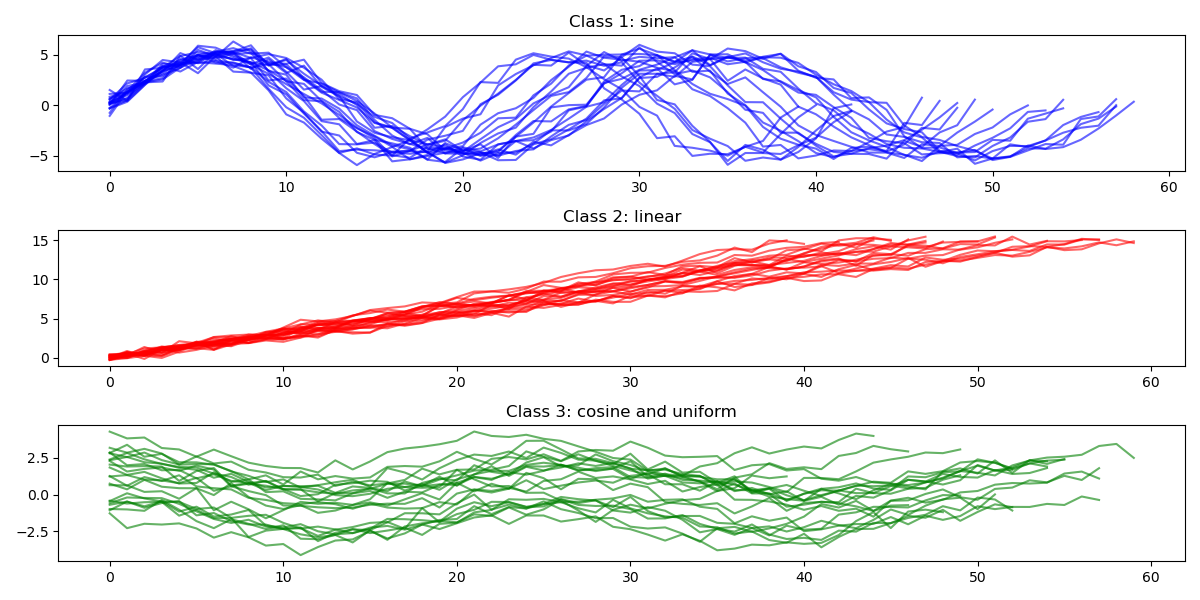
\includegraphics[width=0.9\linewidth]{../Statistical_Sciences_template/figure/Times Series of Three Classes.png}
	\caption{}
	\label{fig:Training}
\end{figure}

\noindent To evaluate the performance of the model, a small test dataset is additionally generated. This test set includes 12 time series in total, with 3 belonging to the first class, 5 to the second class, and 4 to the third. As expected, the time series in the test set were generated from the same underlying distributions as their corresponding classes in the training set, ensuring consistency in the data generating process. The previously described dataset containing 63 time series was used as the training set for fitting the model. After training, the smaller test set was used to evaluate how well the model generalizes to unseen data. The classification results on the test set are summarized in the confusion matrix presented in Figure \ref{fig:confusion_ex}. This figure provides a clear view of the model's predictive performance across the three classes.\\
\begin{figure}[h!]
	\centering
	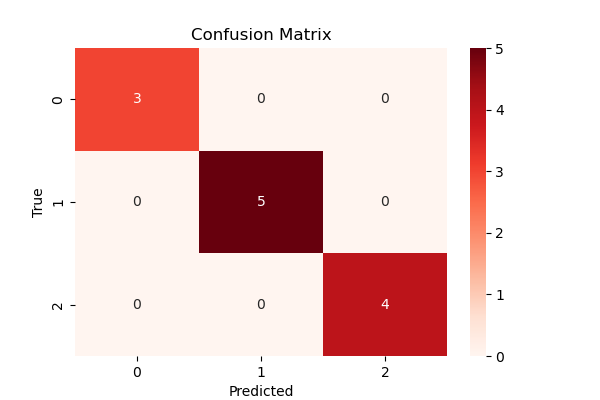
\includegraphics[width=0.9\linewidth]{../Statistical_Sciences_template/figure/Confusion matrix of Shapelet Example.png}
	\caption{From the figure we can see that all observations from the test set are perfectly classified, indicating that the model algorithm can indeed achieve time series classification.}
	\label{fig:confusion_ex}
\end{figure}

\noindent In this experiment, the minimum and maximum allowable lengths for candidate shapelets——denoted as MINLEN and MAXLEN—were set to 3 and 16, respectively. These values were chosen considering both the amount of useful information that can be captured by subsequences and the computational cost of model fitting. Shorter shapelets may fail to capture meaningful patterns, while longer ones can increase fitting time. Thus the maximum depth of the shapelet tree was set to 2, since the simplicity of the dataset and preventing the phenomenon of overfitting.\\
\\
As a result, the final model contains two decision nodes. One node is responsible for identifying instances of the second class, while the other splits between the first and third classes. The overall structure of the tree is visualized in Figure \ref{fig:tree}, which provides a general overview of the model’s decision process. It should be noted that the shapelets and their corresponding optimal split points are not directly visible in Figure \ref{fig:tree}. Although this limits the interpretability of the decision criteria at a better level, the figure still offers valuable insight into how the model is organized and how it partitions the data space during classification.\\
\begin{center}
	\begin{tikzpicture}[
		node distance=2cm,
		level distance=1.5cm,
		sibling distance=4cm,
		every node/.style={draw, circle}
		]
		\node (Root) {all}
		child {node {2}
		}
		child {node {}
			child {node {1}}
			child {node {3}}
		};
		\label{fig:tree}
	\end{tikzpicture}
\end{center}
To provide a more detailed understanding of the model’s structure, we begin by examining the root node of the shapelet tree. At this node, the selected shapelet is a subsequence of length 8, which corresponds to the decreasing red curve shown in Figure \ref{fig:shapetest}. The optimal threshold (i.e., the best split point) associated with this shapelet is approximately 10.024. From visual inspection, it is clear that the shapelet exhibits a generally decreasing pattern. This characteristic reflects the behavior of time series from the first and third classes, both of which contain locally decreasing subsequences. In contrast, time series from the second class are generated from a linearly increasing trend, and therefore they do not include subsequences that resemble the shapelet’s downward slope. As a consequence, the distances between the shapelet and the second class time series are considerably larger than those for the first and third classes. This difference in distance defines the splitting rule for the root node.\\
\begin{figure}[h!]
	\centering
	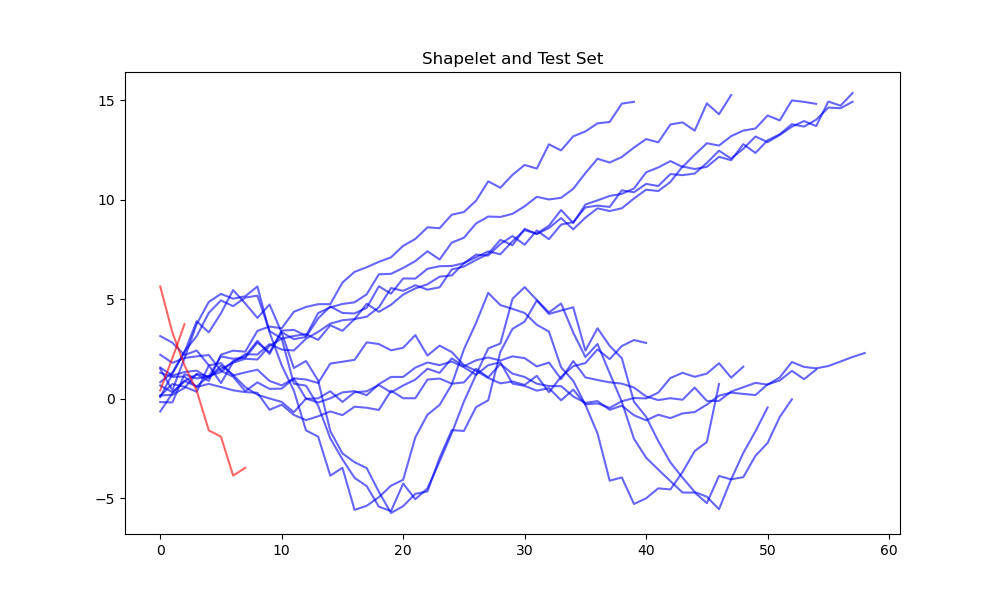
\includegraphics[width=0.9\linewidth]{../Statistical_Sciences_template/figure/Shapelet and Test Set.png}
	\caption{}
	\label{fig:shapetest}
\end{figure}
It is also worth noticing that the threshold value of 10.024 is relatively high. This is mainly due to the fact that the shapelet itself originates from a time series in the first class, which follows a sine function with added noise. Because of the generating sine function’s sharper slope in some regions, the shapelet captures a steep decline. On the other hand, the third class—generated by a cosine function with a uniformly random effects and noise——does not contain subsequences having a similarly steep decline. As a result, the distances between the shapelet and third-class time series are not small, which contributes to the higher threshold at this node.\\
\\
The second decision node, which is for distinguishing between the first and third classes, captures a relatively short shapelet with length 3. The corresponding threshold value of this shapelet is approximately 1.451. Again as shown in Figure~\ref{fig:shapetest} , this shapelet appears to have been extracted from a time series belonging to the first class. It resembles a short, sharply increasing part of the sine function, which is characteristic of the first class’s underlying pattern. Despite its small length, this shapelet is highly effective in separating the two classes. The reason lies in its steep positive slope, which is not commonly found in time series from the third class. Since the third class is generated from a cosine function with an added uniform effect and noise, its local segments tend to vary more gradually and do not frequently contain strong upward trends. Because of this clear difference in local pattern behavior, the distances between this increasing shapelet and the third class time series are larger than those of the first class series. This contrast allows the model to set a relatively low threshold (1.451) and hence compared to the root node's threshold this node's threshold is relatively much smaller.\\
\begin{figure}[h!]
	\centering
	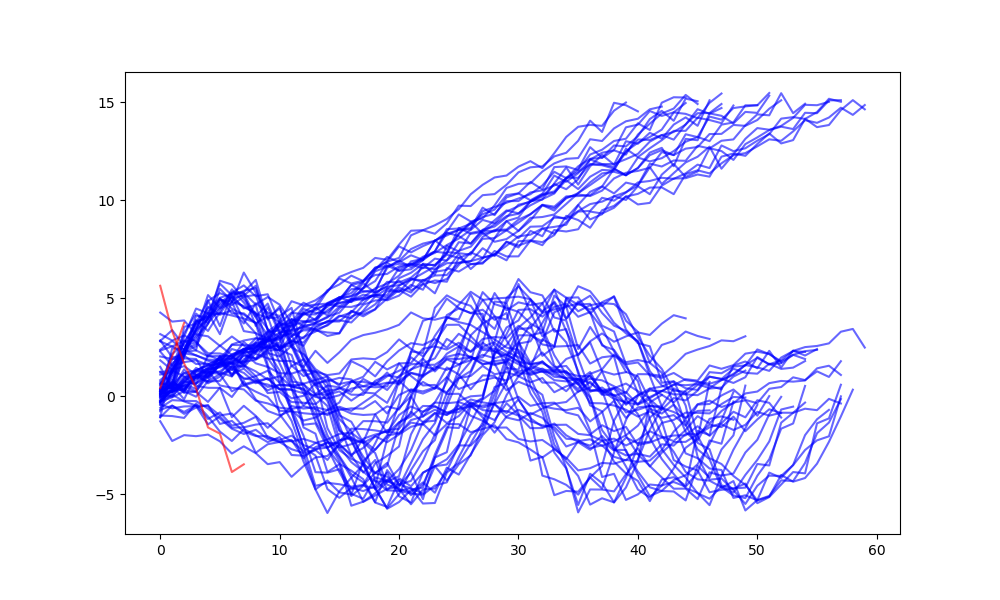
\includegraphics[width=0.9\linewidth]{../Statistical_Sciences_template/figure/Shapelet and Train Set.png}
	\caption{This figure show the shapelets of the model and the original training dataset. It's very clear that the length of time series varies, the short shapelet is quiet close the the sine generating function and also does the long shapelet.}
	\label{fig:shapetrain}
\end{figure}
\subsection{Further Notes and Limitations}\label{subsec:limit}

As mentioned at the beginning of the section, the core idea of this algorithm is derived from the paper published by L. Ye and E. Keogh in 2009. However, since the algorithm was proposed earlier, it is difficult to find a mature and complete ready-made implementation package or library for direct application. To this end, I developed a complete Python implementation from scratch based on the pseudocode provided in the original paper, including core algorithm classes and multiple auxiliary functions. Although these codes can basically implement the core functions described in the paper, due to the short development cycle and some implementation details that need to be improved, the current version still has several obvious limitations: first, in terms of visualization, the existing class implementation lacks the graphical display function of the decision tree model and its node structure; second, the dictionary used to store model features can clearly display the model architecture in the interactive environment of Spyder, but it is difficult to print out normally in the VScode environment; in addition, the current implementation still has some missing functions, such as the failure to fully save the specific location information of the feature shapelet, and only supports two basic metrics, which are Euclidean distance and Manhattan distance, in terms of distance calculation, and has not yet expanded to implement more abundant distance metric options. The specific application instructions of this Python implementation can be found in Appendix \ref{app:A}. \\
\\
In addition, this algorithm has a particularly important systematic problem, that is, the time complexity and space complexity of the algorithm training model are very large. As L. Ye and E. Keogh (2009) wrote, the time complexity of this model is $O(\bar{l}^3n^2)$, where $\bar{l}$ is the average length of the sequence, and $n$ is the number of time series in the training set. The number of possible candidates for a time series should be $\sum_{j=3}^{l_i-1} j$, where $l_i$ is the length of the i-th time series, and $n$ observations may result in a huge number of candidates that is $\sum_{i=1}^n\sum_{j=3}^{l_i-1} j$. In the process of model fitting, if the number of time series observations in the training set is too large and the length is too long, the stored candidates may cause insufficient computer memory and cause the computer to crash. In addition, the algorithm has a structure similar to a multi-classification decision tree, and this structure contains a recursive algorithm. It is difficult to accelerate the recursive algorithm through the GPU. Even if the GPU acceleration is obvious in the process of array processing and time series distance calculation, the entire algorithm still consumes a lot of time in fitting the model.\\
\\
\section{Review of Other Statistical Learning Methods}
Before formally launching the experimental analysis, it is necessary to systematically sort out the concepts of the statistical learning methods to be adopted. This theoretical review can not only lay a solid theoretical foundation for subsequent empirical research, but also help to deeply understand the core ideas of various algorithms and their applicable conditions, thereby ensuring the interpretability of experimental results.\\
\\
The statistical learning methods used in this study can be divided into two categories: supervised learning and unsupervised learning. In the field of unsupervised learning, hierarchical clustering and partitioning around medoids (PAM) are mainly used. In supervised learning, this study focuses on four classic algorithms: K-Nearest Neighbors (KNN), Logistic Regression, Multinomial Logistic Regression, and Support Vector Machine. \\
\\
\subsection{Hierarchical Clustering}
Hierarchical clustering is a classical unsupervised learning algorithm that organizes data into a tree-like structure known as a dendrogram, based on pairwise distances or dissimilarities between observations. The most widely used approach is agglomerative hierarchical clustering, which follows a bottom-up strategy. It begins with each data point as an individual cluster and iteratively merges the two closest clusters until all points are grouped into a single cluster. \\
\\
Although Euclidean distance and Manhattan distance are commonly used metrics, correlation-based dissimilarity is also frequently employed, which can be defined as:\\
\begin{equation}
	d_C(\boldsymbol{x_1},\boldsymbol{x_2})=\frac{1}{2}(1-r(\boldsymbol{x_1},\boldsymbol{x_2}))
\end{equation}
where $r(\boldsymbol{x_1},\boldsymbol{x_2})$ denotes the Pearson correlation coefficient between $\boldsymbol{x_1}$ and $\boldsymbol{x_2}$.\\
\\
Once the dissimilarity matrix is computed, different linkage criteria can be used to determine the distance between clusters:\\
\begin{itemize}
 \item Single linkage takes the minimum pairwise distance between elements of two clusters:
  $$d(C_1,C_2)=\min_{\boldsymbol{x_1} \in C_1, \boldsymbol{x_2} \in C_2} d(\boldsymbol{x_1},\boldsymbol{x_2})$$,
 \item Complete linkage takes the maximum pairwise distance between elements of two clusters:
  $$d(C_1,C_2)=\max_{\boldsymbol{x_1} \in C_1, \boldsymbol{x_2} \in C_2} d(\boldsymbol{x_1},\boldsymbol{x_2})$$ and
 \item Average linkage takes the mean of all pairwise distances between elements in two clusters:
  $$d(C_1,C_2)=\frac{1}{|C_1||C_2|}\sum_{\boldsymbol{x_1} \in C_1, \boldsymbol{x_2} \in C_2} d(\boldsymbol{x_1},\boldsymbol{x_2})$$
\end{itemize}
Each linkage method leads to a different hierarchical structure and thus different clustering results. The final output dendrogram represents the hierarchy of clusters and can be used to identify the most natural grouping of the data by cutting the tree at a specific level.\\
\\
\subsection{Partitioning Around Medoids}\label{subsec:PAM}
PAM (Partitioning Around Medoids) is a robust clustering algorithm that, like K-Means, partitions data into K clusters through iterative optimization. However, a key distinction lies in the choice of cluster centers: PAM uses actual sample points—called medoids—as centers, rather than computed means.\\
\\
A medoid is defined as the data point within a cluster that has the minimum total dissimilarity (or distance) to all other points in that cluster. Unlike centroids in K-Means, medoids must be real observations from the dataset, enhancing the robustness of the algorithm. Mathematically, the medoid of cluster $C_k$ s computed as:\\
\begin{equation}
	\boldsymbol{m_k}=\arg \min_{\boldsymbol{x} \in C_k} \sum_{\boldsymbol{y} \in C_k} d(\boldsymbol{x},\boldsymbol{y})
\end{equation}
where $d(.,.)$ denotes the chosen distance metric.
Thus the goal is to minimize the total distance from all sample points to the center of the cluster to which they belong, that is:\\
\begin{equation}
	Total\textunderscore Cost=\sum_{k=1}^K\sum_{\boldsymbol{x} \in C_k} d(\boldsymbol{x},\boldsymbol{m_k})
\end{equation}
where K denotes the number of clusters and $\boldsymbol{m_k}$ is the medoid pf cluster $C_k$.\\
Both PAM and K-Means aim to minimize intra-cluster dissimilarity and cluster data points to the nearest center. However, the critical difference is located in how the cluster centers are defined. K-Means uses the centroid, calculated as the mean of all points in the cluster. This approach is computationally efficient and intuitive but highly sensitive to outliers, since a single extreme value can break a mean down and influence the result significantly. In contrast, PAM selects a real data point as the medoid, making it more robust to noise and less influenced by outliers.\\
\\
Another advantage of PAM is its flexibility with distance metrics. While K-Means relies on Euclidean distance and assumes clusters to be convex, PAM allows for a wilder range of distance metrics (e.g. Manhattan or cosine distance), which is better handling complex datasets.\\
\\
The limitations of K-Means become particularly evident in high-dimensional settings, that is when $(p>>n)$. Due to the curse of dimensionality, the Euclidean distance becomes less discriminative in high-dimensional space, resulting in a significant decrease in the clustering effect of K-Means. In addition, samples in high-dimensional data are usually sparse, and mean calculation is easily disturbed by outliers or irrelevant features, making the mean unrepresentative. In contrast, PAM is more robust to outliers and redundant features of high-dimensional data because it clusters based on actual data points.\\
\\
\subsection{Lasso for Logistic Regression}\label{subsec:LR}
Lasso for logistic regression, also known as logistic regression with an L1 penalty, is a fundamental statistical learning method that performs both variable selection and classification simultaneously. It extends standard logistic regression by introducing a regularization term that penalizes the absolute values of the regression coefficients. As a result, some of the coefficients will be shrunk exactly to zero. This approach is especially useful in high-dimensional situations——particularly when the number of variables $p$ is much larger than the number of observations $n$, i.e., in cases where $p>>n$. In such situations, lasso helps prevent overfitting. Another advantage of this method is its high interpretability. Since the model tends to retain only a subset of the most informative variables, it becomes easier to understand which features are making great influences.\\
\\
For logistic regression, the corresponding distribution is the binomial distribution, whose probability mass function is $f(p)=\binom{n}{k} p^k(1-p)^{n-k}$. The exponential family form of this function is:\\
\begin{equation}
f(p)=\exp(k\ln \frac{p}{1-p}+n\ln(1-p)+\ln C)
\label{binomial}
\end{equation} 
where $C$ is the constant part.\\
\\
The canonical link function here is $\eta=\frac{p}{1-p}$ where $\eta$ represents the systematic component, i.e. $\eta=\boldsymbol{X}\beta$. We can maximize the log-likelihood function of the $n$ times of Bernoulli trials to estimate the coefficients, that is\\ 
\begin{equation}
l=\sum_{k:y=1}\ln p_k\sum_{k:y=0}\ln(1-p_k)=\sum_{i=1}^n [y_i\ln p_i+(1-y_i)\ln(1-p_i)]
\label{LRlikelihood}
\end{equation}
The negative of the log-likelihood function shown in Equation \eqref{LRlikelihood} corresponds to the standard definition of binary cross entropy. Hence we can also define the loss function of logistic regression using:\\
\begin{equation}
loss=\sum_{i=1}^n [-y_i\ln p_i-(1-y_i)\ln(1-p_i)]
\end{equation}
The procedures are consistent because maximizing the log-likelihood is equivalent to minimizing the entropy of the predicted probabilities. When we apply L1 regularization to logistic regression the estimation of coefficients is modified by adding a penalty term that constrains the absolute value of the coefficients. In this case, the coefficients are estimated by maximizing the following penalized log-likelihood\\
\begin{equation}
	l=\sum_{i=1}^n [y_i\ln p_i+(1-y_i)\ln(1-p_i)]-\lambda \sum_{j=1}^p |\beta_j|
\end{equation}
Equivalently, this can be framed as minimizing the regularized loss function:
\begin{equation}
	loss=\sum_{i=1}^n [-y_i\ln p_i-(1-y_i)\ln(1-p_i)]+\lambda \sum_{j=1}^p |\beta_j|
\end{equation}
The regularization term $\lambda \sum_{j=1}^p |\beta_j|$ encourages sparsity in the model by shrinking less important coefficients to zero, which helps with both feature selection and generalization, especially in high-dimensional datasets.\\
\\

\subsection{Lasso For Multinomial Logistic Regression}\label{subsec:MLR}
Lasso for multinomial logistic regression is also a statistical learning method that performs both variable selection and classification simultaneously as lasso for logistic regression. However, the underlying probability distribution in this case is different. The multinomial logistic regression model is based on the multinomial distribution, whose probability mass function is $f(p_1,...,p_k)=\frac{n!}{x_1!...x_k!} p_1^{x_1}...p_n^{x_n}$, whose exponential family form can be expressed as:\\
\begin{equation}
	f(p_1,...,p_k)=\exp[\sum_{i=1}^k x_i\ln p_i+\ln n!-\sum_{i=1}^k\ln x_i!]=\exp[(\ln\boldsymbol{p})^T\boldsymbol{x} +\ln n!-\sum_{i=1}^k\ln x_i!]
\end{equation}
where $\boldsymbol{p}=(p_1,...,p_k)$ is the vector of class probabilities and $\boldsymbol{x}=(x_1,...,x_k)$ is the corresponding counts. The canonical link function is $\boldsymbol{\eta}=\ln\boldsymbol{p}$, i.e. $\eta_i=\ln p_i$. Due to the constraint that all probabilities must sum to 1, that is $\sum_{i=1}^k p_i=1$, equivalently:
\begin{equation}
 	\sum_{i=1}^k e^{\eta_i}=1
\end{equation}
From this, we easily can derive the inverse of the link function, which is widely known as the softmax function:\\
\begin{equation}
	p_i=\frac{e^{\eta_i}}{\sum_{i=1}^k e^{\eta_i}}
\end{equation}\\
The corresponding log-likelihood function takes the form:\\
\begin{equation}
	l=\sum_{i=1}^{n}\sum_{j=1}^k \boldsymbol{1}(x_i=k)p_k
\end{equation}
where $\boldsymbol{1}(x_i=k)$ is the indicator function, is the indicator function, which equals 1 if the i-th observation belongs to class $k$, and 0 otherwise.\\
\\ 
Similar to the binary logistic regression case, the loss function is the negative of the log-likelihood, which corresponds to the cross entropy loss used in multi-class classification:\\
\begin{equation}
	loss=-\frac{1}{n}\sum_{i=1}^{n}\sum_{j=1}^k \boldsymbol{1}(x_i=k)p_k
\end{equation}
If the L1 regularization is introduced, the maximum likelihood estimation will be:
\begin{equation}
	l=\sum_{i=1}^{n}\sum_{j=1}^k \boldsymbol{1}(x_i=k)p_k-\lambda \sum_{j=1}^{k}\sum_{m=1}^{p}|\beta_{jm}|
\end{equation}
And equivalently, the regularized loss function to minimize is:
\begin{equation}
	loss=-\sum_{i=1}^{n}\sum_{j=1}^k \boldsymbol{1}(x_i=k)p_k+\lambda \sum_{j=1}^{k}\sum_{m=1}^{p}|\beta_{jm}|
\end{equation}
It is also worth noting that when the number of classes $k=2$, the model will degenerate into the typical logistic regression.\\
\\

\subsection{K-Nearest Neighborhood}\label{subsec:knn}
The K-nearest neighbors (KNN) algorithm is one of the most fundamental statistical learning methods, whose core idea is quite intuitive: observations that are close to each other in the feature space are likely to belong to the same class. In other words it means that similar observations are more likely to classified together. Therefore, two main concepts are of vital importance how the KNN algorithm works: similarity (or distance) and the number of neighbors, denoted by K. \\
\\
In terms of measuring similarity between observations, several distance metrics can be used, where the choice of metric may significantly affect the performance depending on the characteristics of the data. Common options include the Euclidean distance, Manhattan distance, or more generally, the Minkowski distance, where different values of the power parameter $p$ can adjust the behavior of the metric. However, when dealing with datasets that have a high number of dimensions, cosine similarity often performs well. This can be extremely useful when the absolute values vary a lot but the overall pattern is more informative. Cosine similarity is mathematically defined as:\\
\begin{equation}
	similarity(\mathbf{x_1},\mathbf{x_2})=\frac{\mathbf{x_1} \cdot \mathbf{x_2}}{\| \mathbf{x_1} \| \| \mathbf{x_2} \|}
\end{equation} 
where $\mathbf{x_1}$ and $\mathbf{x_2}$ are two data points in the feature space, and the numerator is their dot product while the denominator is the product of their $L^2$ norms.\\
\\
Another crucial aspect is selecting an appropriate value for K, that is the number of neighbors. This parameter plays a major role in determining the performance of the model. If K is too small, for example, K=1, the model may suffer from high variance, meaning it becomes very sensitive to noise and outliers, which could lead to overfitting, where the model fits the training data too well but fails to generalize to other data. While if the K is too large, there will be hish risk that the model may underfit the training data. In such cases, it leads to high bias and poor performance because it averages over too many neighbors, some of which may belong to other classes. \\
\\
To find a suitable value for K, a common strategy is to use a validation dataset to compute classification accuracies or error rates for different choices of K. The optimal K is typically selected as the model that obtained the highest accuracy or equivalently, the lowest classification error. Alternatively, model selection techniques like cross-validation or leave-one-out cross-validation can also be employed.\\
\\
In summary, KNN is simple but powerful, and by carefully choosing both the similarity measure and the number of neighbors, it can be adapted to various types of data and be reasonably interpreted.\\
\\

\subsection{Support Vector Machine and Linear Support Vector Classifier}\label{subsec:SVM}
Support Vector Machine (SVM) is a powerful supervised learning algorithm, mainly used for classification (binary and multi-classification) and regression tasks. Its core idea is to find the optimal decision boundary to maximize the sample interval between different categories. The goal of SVM is to find a hyperplane, which is a decision boundary in n-dimensional space that separates samples of different categories and maximizes the margin, which is the minimum distance from the hyperplane to the nearest sample (support vector).\\
\\
In the linear case, the objective of a SVM is to find a separating hyperplane that best distinguishes between classes. This hyperplane is mathematically represented as:\\
\begin{equation}
	\mathbf{w}^T\mathbf{x}+b=0
\end{equation}
where $\mathbf{w}$ is the weight vector (or coefficient vector) and $b$ is the shift term. The offset of the hyperplane from the origin is determined by $\frac{b}{\|w\|}$. For an observation to be correctly classified, it must satisfy the condition:\\
\begin{equation}
	y_i(\mathbf{w}^T\mathbf{x}+b) \geq0
	\label{margin1}
\end{equation}
This expression ensures that each point lies on the correct side of the hyperplane, depending on its label $y_i \in \{-1,1\}$.\\
\\
The goal of the SVM algorithm is to maximize the margin, which is defined as the smallest distance from the hyperplane to training samples. In other words, SVM seeks the hyperplane that achieves the largest possible margin between the classes. For data that can be linearly separated, this concept is formalized by introducing hard margins, which are two parallel hyperplanes placed on either side of the decision boundary, such that no observations fall between them. In this case, Equation \eqref{margin1} represents:
\begin{equation}
		y_i(\mathbf{w}^T\mathbf{x}+b) \geq 1
\end{equation}
Under this constraint, the optimization problem becomes:\\
\begin{equation}
	\min_{\|\mathbf{w}\|,b}\frac{1}{2}\|\mathbf{w}\|^2
\end{equation}
where $\|\mathbf{w}\|$ denotes the L2 norm of the weight vector. This objective function minimizes the norm of the weight vector, effectively maximizing the margin.\\
\\
In real-world datasets, however, perfect linear separability is often not achievable. To accommodate misclassifications or marginal violations, slack variables $\epsilon_i$ are introduced. These variables allow certain observations to lie within or on the wrong side of the margin boundary, offering flexibility in fitting training data. The optimization then becomes:\\
\begin{equation}
\begin{split}
& \min_{\|\mathbf{w}\|,b,\epsilon}\frac{1}{2}\|\mathbf{w}\|^2+C\sum_{i=1}^n \epsilon_i \\
& \text{s.t.} \qquad y_i(\mathbf{w}^T\mathbf{x}+b) \geq 1-\epsilon_i \qquad \epsilon_i \geq 0
\end{split}
\label{svmL2}
\end{equation}
where $C$ is a non-negative tuning parameter that controls the trade-off between maximizing the margin and minimizing classification error. A higher value of $C$ emphasize more on minimizing misclassification, while a lower value emphasizes a larger margin. \\
\\
In high-dimensional settings—particularly when the number of features is large relative to the number of observations—using an L1 penalty instead of an L2 penalty can lead to improved generalization. This is because the L1 norm promotes sparsity in the solution, effectively performing feature selection by shrinking some coefficients to exactly zero. The optimization problem in Equation \eqref{svmL2} becomes:\\
\begin{equation}
\begin{split}
& \min_{\|\mathbf{w}\|,b,\epsilon}\frac{1}{2}\|\mathbf{w}\|+C\sum_{i=1}^n \epsilon_i \\
& \text{s.t.} \qquad y_i(\mathbf{w}^T\mathbf{x}+b) \geq 1-\epsilon_i \qquad \epsilon_i \geq 0
\end{split}
\label{svmL1}
\end{equation}
where $\|w\|$ denotes the L1 norm of the weight vector. The L1 penalty will cause some weights to become 0, resulting in a sparse weight vector and selecting features automatically. Hence the model will be more robust to outliers and noise.


\chapter{Experiment}
For the experiment, the dataset used is the well-known and widely adopted GTZAN dataset, which is a standard benchmark in the fields of music information retrieval, genre classification, and related audio analysis tasks. The dataset consists of 1000 audio signal files, containing 10 distinct music genres, with 100 samples per genre. Each audio signal file is approximately 30 seconds in duration, sampled at a rate of 22050 Hz, and stored in 16-bit mono .wav format. The use of mono rather than stereo recordings simplifies audio processing and avoids complications when analyzing multichannel audio signals.\\
\\
The GTZAN dataset was originally curated by the Marsyas Music Information Retrieval Toolkit and has become a canonical reference in evaluating the effectiveness of various music classification algorithms. Additional information about the dataset is provided in Appendix B (\ref{app:B}).
\\
However, due to limitations in computational resources and the computational complexity of the shapelet tree-based algorithm employed in this study, only a subset of the dataset was used for experiment. That is, the analysis was limited to four genres: classical, disco, hiphop, and metal. As a result, the dataset was reduced to 400 audio samples, making the classification task from a 10-class problem to a 4-class problem. \\
\\
\section{Exploratory Analysis of the Data}
\subsection{Description of Data}
As mentioned earlier, each music signal in the dataset is approximately 30 seconds in duration, with a sampling rate of 22050 Hz. This implies that each second contains 22050 samples, resulting in roughly 660000 data points per file. Consequently, each observation is represented as a high-resolution, long-step time series, which poses significant challenges for direct processing of raw audio signals. \\
\\
To address this, I extracted a 20-second segment starting from the 5th second of each audio file to represent the entire sample. This preprocessing step was motivated by three main considerations:
\begin{quote}
	1.Sufficiency for Genre Recognition: For human listeners with basic music knowledge, a 20-second-long piece of music is enough to identify the genre of a file.\\
	\\
	2.Reduction of Computational Load: Shortening the length of the audio signals significantly reduces computational complexity during feature extraction and model training. This is especially important given the processing requirements of shapelet tree-based algorithm.\\
	\\
	3.Avoidance of Calculation Problems: Some audio files contain initial pauses or segments of silence, lasting from one to several seconds. These parts yield samples with all-zero values, which can influence feature extraction processes. In particular, statistics that rely on second-order moments or higher order moments—such as variance or autoregressive coefficients—can be severely affected by these zero-valued regions, leading to inaccurate or undefined results.
\end{quote}
Hence, the data used in this study consists of audio signal segments extracted from the 5-th second to the 25-th second of each file. Although these segments have uniform duration——each being exactly 20 seconds——they are not temporally aligned across samples. This lack of alignment arises due to natural variations in the starting point of musical and differences in tempo or rhythmic structure. In other words, the beginning of the selected segment may capture different musical phrases or structures across samples, depending on the genre, composition and music itself. As a result, direct comparisons between raw signals may be less meaningful, since similar patterns might occur at different time positions across different files. \\
\\

\subsection{Feature Project}\label{subsec:FP}
After obtaining the 400 audio signal segments, each with a duration of 20 seconds, the next step was to compute the MFCCs for each segment. This transformation is a critical step in audio signal processing, as MFCCs capture the timbral characteristics of sound and are widely used in tasks such as speech and music genre classification. Thus it is the main topic of this study. \\
\\
Before extracting the MFCCs, several key parameters must be defined: the frame length, the hop length, and the analysis window length. These parameters control how the audio signal is divided and analyzed over time. A general description of how these parameters influence the feature extraction process was previously provided in Section \ref{subsec:framingwindowing}; here, I will elaborate on their specific functions and roles within the context of this experiment.\\
\begin{quote}
	1.Frame length determines the duration of each short-time frame over which the Fourier Transform is applied. This frame is to satisfy the assumption that the time series are stationary in weak statistical sense.\\
	\\
	2.Hop length is the number of samples between the starts of consecutive frames. This controls the overlap between frames and ultimately affects the temporal resolution of the extracted features.\\
	\\
	3. Length of each analysis window specifies the segment of time over which summary statistics (e.g., mean, variance, range) are computed from the MFCCs. For instance, a one-second analysis window must encompass multiple overlapping frames to enable accurate statistical characterization. 
\end{quote}
In my experiment, I used two different durations for the analysis window: 1 second and 0.4 seconds. For each of these, two frame lengths were selected—2048 samples and 1024 samples—to segment the signal. Additionally, different hop lengths of 512, 256, and 128 samples were tested to assess their effect on feature extraction and overall model performance. The detailed configuration of these experimental settings is summarized in Table \ref{table: FeatureProjectStructureofDatasets}: 
\begin{table}[H]
	\centering
	\caption{Feature Project Structure of Datasets}\label{table: FeatureProjectStructureofDatasets}
	\begin{tabularx}{\linewidth}{>{\raggedright\arraybackslash}X m{3.75cm} m{3.75cm} m{3.75cm}}
		\toprule
		Hop Length     & 512 & 256 & 128  \\ \midrule
		2048     &    \ding{51}         &    \ding{51}         &   \ding{55}                           \\
		1024     &    \ding{55}         &    \ding{51}         &   \ding{51}                           \\	\bottomrule
	\end{tabularx}
\end{table}
\noindent This table shows that four distinct datasets were constructed, each corresponding to a specific configuration of frame length and hop length. These combinations determine how the audio signal is framed and how densely the temporal features are sampled within each analysis window.\\
\\
To clarify this setup, let us take the dataset with a one-second analysis window, a frame length of 2048 samples, and a hop length of 512 samples as an example. Since the sampling rate for all audio signals is 22050 Hz, each second of audio contains 22050 samples. The duration of a single frame of 2048 samples is: $\frac{2048}{22050}\approx0.0929$, which is approximately $92.9$ milliseconds. However, constructing a one-second window is not as simple as stacking $\frac{22050}{2048} \approx 11$ frames. Due to the overlapping structure introduced by the hop length, the actual number of frames that construct a one-second analysis window must be calculated using the formula defined in Equation \eqref{windownumber}. Accordingly, the number of frames in this is:
$$
\lceil \frac{22050*1-2048}{512}+1\rceil=41
$$
By default, 13 MFCCs are computed for each audio segment, as illustrated in the example shown in Figure \ref{fig:MFCC Example}. As previously mentioned, each audio segment used in the experiment is 20 seconds long. Consequently, the MFCCs extracted from each audio signal form a matrix of size $13 \times p$, where the number of columns $p$ depends on several key parameters: the frame length, hop length, and analysis window length.\\
\\
The exact value of $p$—i.e., the number of frames that can be extracted from a 20-second audio segment——can be calculated using Equation \eqref{windownumber}, which accounts for overlapping frames due to the hop length.\\
\\
For instance, if the frame length is 2048 samples and the hop length is 512 samples, the resulting MFCC matrix will be of size $13 \times 859$. On the other hand, if the frame length is reduced to 1024 samples and the hop length to 128 samples, then a denser frame extraction is achieved, yielding a much larger matrix of size $13 \times 3439$. \\
\\
When each observation is represented by a $13 \times 3439$ MFCC matrix, it becomes a significant challenge for many traditional statistical models due to the high dimensionality of the input. Although neural networks are capable of handling such high-dimensional data, they are not employed in this study. Therefore, a dimensionality flattenation strategy was used to extract summary statistics from the MFCCs within each analysis window. For each MFCC in an analysis window, five statistical measures were computed specially: mean, variance, range, skewness and kurtosis. Since there are 13 MFCCs, this results in $5 \times 13 = 65$ features per analysis window.\\
\\
For datasets using a one-second-long analysis window, there are 20 non-overlapping windows within a 20-second audio segment. Thus, each observation is represented by a feature vector of size $65 \times 20 = 1300$. In contrast, for datasets using a 0.4-second-long analysis window, a total of $20 / 0.4 = 50$ windows can be extracted per audio sample. Accordingly, the number of resulting features becomes $65 \times 50 = 3250$. As a result, each audio observation is ultimately transformed into a 1300-dimensional vector in the case of the one-second analysis window and a 3250-dimensional vector in the case of the 0.4-second analysis window.\\
\\
In summary:
\begin{itemize}
	\item Each 20-second audio observation is transformed into a 1300-dimensional vector when using a one-second analysis window.
	\item Each observation becomes a 3250-dimensional vector when using a 0.4-second analysis window.
\end{itemize}
This transformation yields a structured one-dimension representation of each audio signal, making it more suitable for downstream tasks such as clustering or classification using conventional statistical learning techniques.\\
\\
\subsection{Clustering}\label{subsec:clustering}
After obtaining the statistical feature matrix of MFCCs through the steps above, the next study goal is to conduct cluster analysis on each observation sample corresponding to the matrix to explore the potential data structure pattern. However, in the actual operation process, the first key challenge is the dimensionality disaster problem of the feature matrix, that is, the variable dimension $p$ of the matrix significantly exceeds the number of observation samples $n$, forming a typical $p>>n$ high-dimensional data scenario. The characteristics of this data structure will cause many traditional statistical methods to fail in this situation. The fundamental reason is that the geometric characteristics in high-dimensional space are essentially different from those in low-dimensional space.\\
\\
Specifically, in terms of distance measurement, Mahalanobis distance is a standardized distance measurement that considers the covariance structure of variables. Its calculation process relies on the inverse operation of the covariance matrix. However, under the condition of $p>>n$, the sample covariance matrix must be singular, which cannot meet the requirements of a positive definite matrix, resulting in the non-existence of the inverse matrix. This mathematical property makes the calculation of Mahalanobis distance theoretically infeasible.\\
\\
Similar problems are more prominent in clustering methods based on probability models, such as Gaussian mixture model (GMM) and t-mixture model (t-MM). When such models use the expectation maximization (EM) algorithm to estimate parameters, it is necessary to calculate the determinant of the high-dimensional covariance matrix and its inverse matrix. When $p>>n$, the singularity of the covariance matrix will cause numerical instability in the log-likelihood function, making it impossible for the EM algorithm to converge to the global optimal solution, and the final clustering result will seriously deviate from the actual data structure.\\
\\
For the K-means clustering algorithm, the challenges brought by high-dimensional space cannot be ignored. According to the theory of the curse of dimensionality, as the dimension increases, the distribution of data points in high-dimensional space will become extremely sparse, resulting in the Euclidean distance between any two points becoming similar. This phenomenon will seriously weaken the distance discrimination that the K-means algorithm relies on, making it easy for the iterative process to fall into the local optimal solution and produce pseudo clustering results. What's more serious is that in ultra-high-dimensional space, a large number of feature dimensions may only contain random noise or redundant information. As mentioned in Section \ref{subsec:PAM}, the traditional K-means algorithm uses an isotropic distance metric, which cannot automatically identify and suppress the interference of irrelevant features. Instead, it will equally amplify the noise influence of all dimensions, and ultimately cause the cluster center to deviate from the true subspace distribution structure. \\
\\
Considering the limitations of traditional distance metrics in high dimensional data environments, this study ultimately uses Manhattan distance (L1 distance) and correlation dissimilarity as core similarity metrics, while retaining the clustering results of Euclidean distance (L2 distance) as a benchmark. The choice of this kind of distance measurement strategy is based on mathematical principles and practical application considerations: Manhattan distance is more robust in high dimensional space, and its sensitivity to outliers is significantly lower than that of Euclidean distance. This is because if we regard the L1 norm as a loss function, then its influence function as a statistic is bounded. The correlation coefficient difference can effectively capture the pattern similarity between MFCC feature vectors. By calculating the dissimilarity matrix obtained by subtracting the Pearson correlation coefficient from 1 and times $\frac{1}{2}$, the absolute numerical differences between features can be ignored.\\
\\
In terms of the selection of clustering algorithms, this study uses two distance matrix-based methods, hierarchical clustering and partition around medoids (PAM), instead of relying on parameterized models of the original feature space. This decision has multiple advantages: first, these two methods only need to input a pre-calculated distance matrix to perform clustering, perfectly avoiding numerical calculation problems such as the irreversibility of the covariance matrix under high-dimensional data; second, as described in Section \ref{subsec:PAM}, the PAM algorithm constructs actual observation points as medoids, which is naturally robust to outliers compared to virtual center-based methods such as K-means. When there are abnormal samples in the data, the medoid selected by PAM can still maintain the representativeness of the main data distribution, and will not be influenced by extreme values like the K-means center.\\
\\
In determining the key parameter of the optimal number of clusters $K$, this study uses the average silhouette width (ASW) as an evaluation indicator. This method provides an objective basis for the selection of the number of clusters by systematically measuring the compactness and separation of the cluster structure. The mathematical definition of the Silhouette coefficient is as follows: For any sample i, the calculation formula of its coefficient s(i) is:\\
\begin{equation}
	s(i)=\frac{b(i)-a(i)}{\max(a(i),b(i))}
\end{equation}
where the numerator b(i)-a(i) reflects the advantage of the degree of separation between the sample and the nearest neighbor cluster relative to the degree of cohesion within the cluster, and the maximum value of the denominator is normalized to ensure that the coefficient value always falls within the standardized interval of [-1, 1]. \\
Specifically, a(i) is defined as:\\
\begin{equation}
	a(i)=\frac{1}{|\boldsymbol{C_k}|-1}\sum_{j\in \boldsymbol{C_k},j\neq i} d(i,j)
\end{equation}
which represents the average dissimilarity between sample i and other members of the cluster (i.e., the degree of intra-cluster dispersion). The smaller its value, the stronger the association between the sample and the members of the same cluster. b(i) is defined as: \\
\begin{equation}
	b(i)=\min_{l\neq k}\Bigg(\frac{1}{|\boldsymbol{C_l}|}\sum_{j\in \boldsymbol{C_l}}d(i,j)\Bigg)
\end{equation}
which represents the average distance from sample i to all samples in the nearest neighbor cluster (i.e., the degree of inter-cluster separation). The larger its value, the clearer the cluster boundary. When s(i) is close to 1, it means that sample i is not only highly similar to samples in the same cluster, but also significantly different from neighboring clusters. At this time, the clustering structure is most ideal.\\
\\
The average silhouette width is taken as the arithmetic mean of the Silhouette coefficients of all samples, that is:\\
\begin{equation}
	ASW=\frac{1}{N}\sum_{i=1}^N s(i)
\end{equation}
This study calculates the ASW values corresponding to different preset clustering numbers $K$, and determines the $K$ that makes ASW reach the global maximum as the optimal clustering number. The advantages of this method are: first, its evaluation process does not rely on any distribution assumptions and is applicable to clustering structures of any shape; moreover, the standardized coefficient values can directly compare the quality of results under different clustering algorithms or distance metrics.\\
\\
In order to intuitively present the results of cluster analysis, this study uses multidimensional scaling (MDS) technology to reduce the high-dimensional distance matrix to two-dimensional space for visualization. The MDS algorithm maintains the relationship between the distances of samples before and after dimensionality reduction by optimizing the stress function. In practice, the stress results are almost always less than 0.05, so it can be considered that MDS reflects the distance relationship between observations very well. Moreover, different clusters of observations obtained by clustering are displayed in the two-dimensional MDS plots with different colors.\\
\\
\begin{figure}[H]
	\centering
	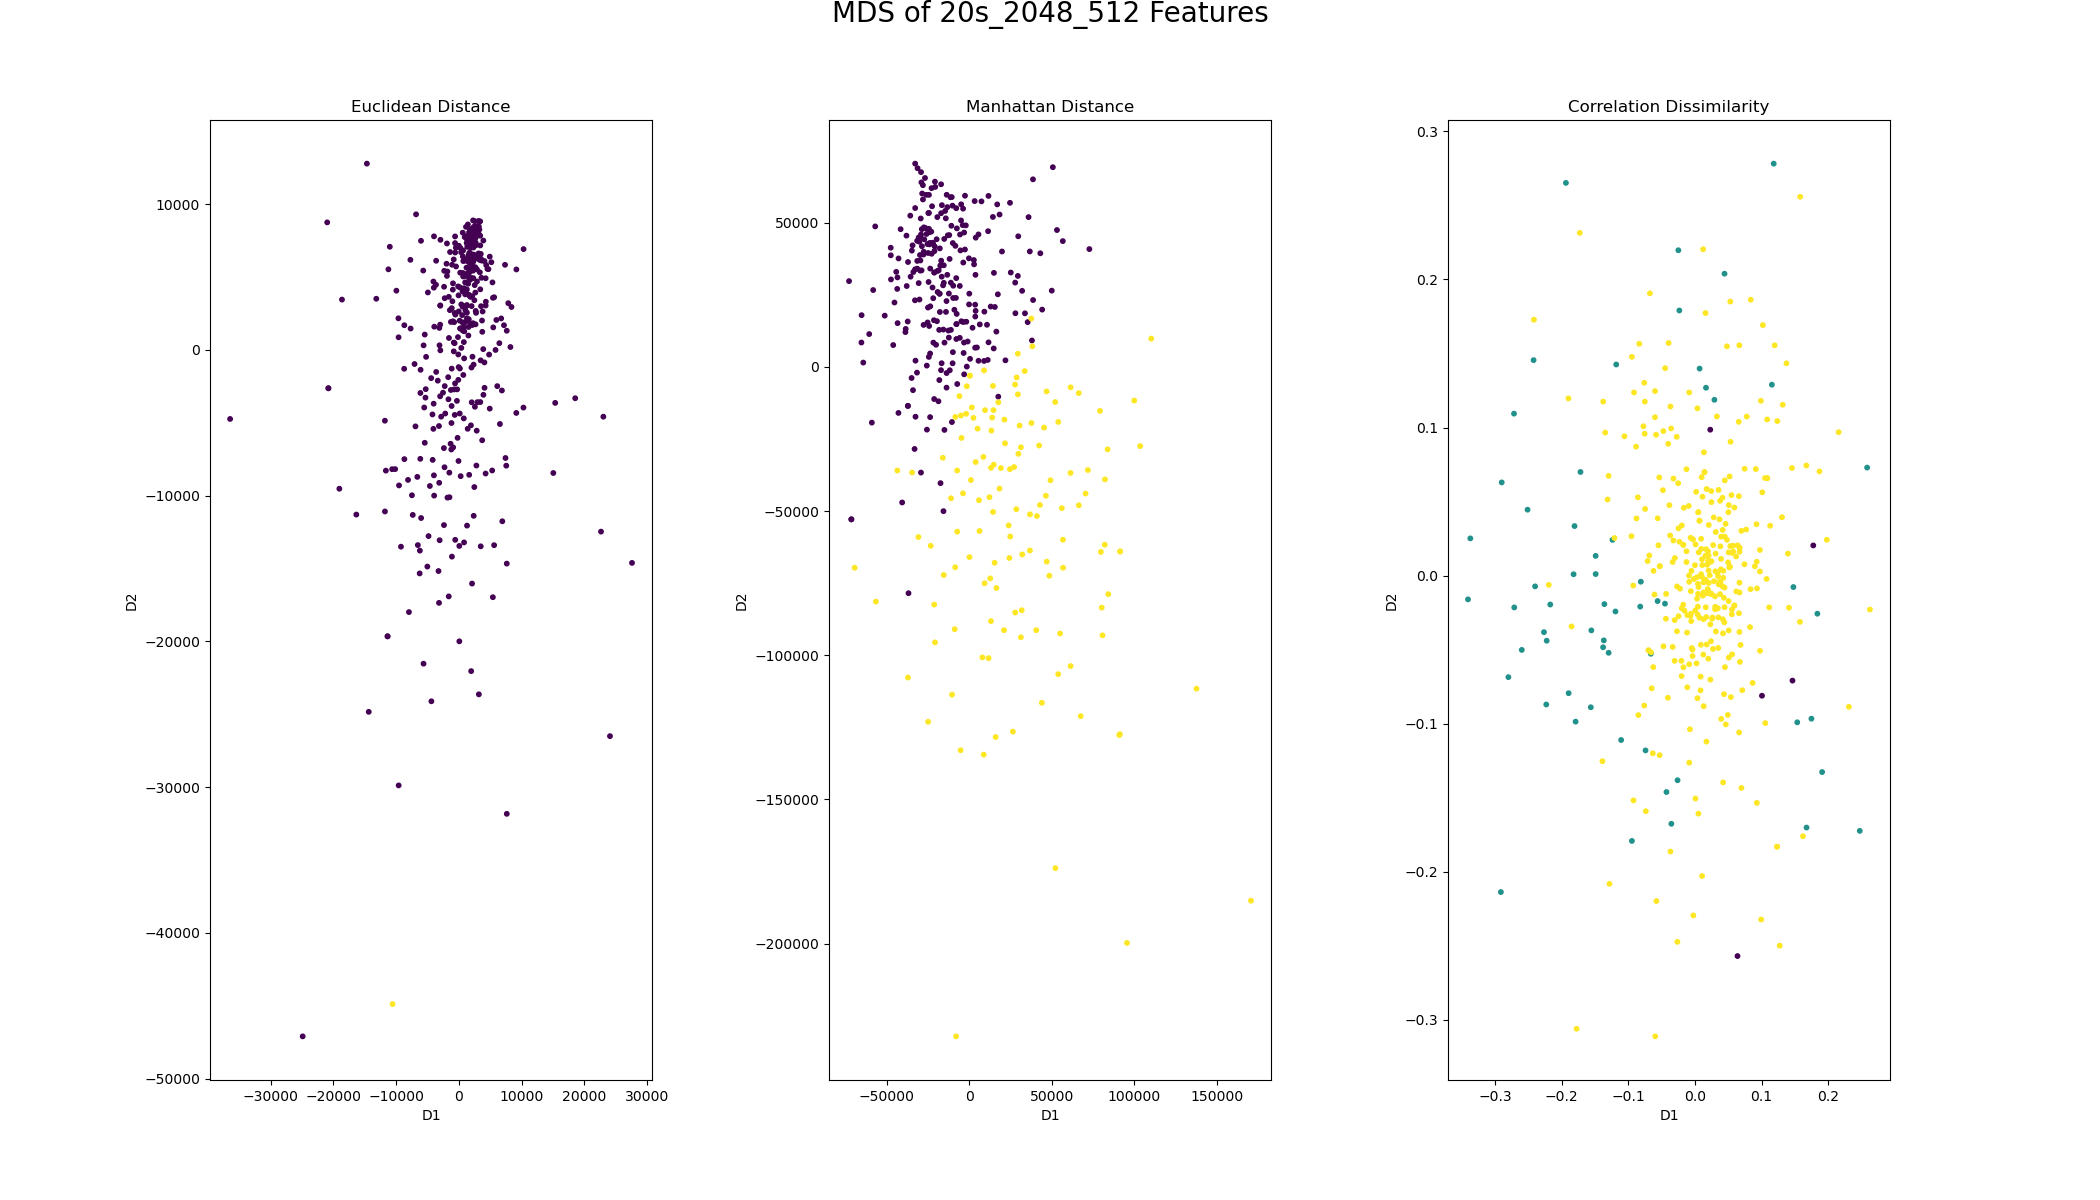
\includegraphics[width=0.9\linewidth]{../Statistical_Sciences_template/figure/MDS of 20s_2048_512 Features Using Complete Linkage.png}
	\caption{The plot is the two-dimensional MDS results of the dataset within 20 seconds, 2048 samples of frame length and 512 samples of hop length for Euclidean distance, Manhattan distance and Correlation dissimilarity respectively.}
	\label{fig:MDS of 20s_1024_256 Features Using Complete Linkage}
\end{figure}
\noindent This figure shows the comparison of clustering results based on different distance metrics (Euclidean distance, Manhattan distance, and correlation dissimilarity) when using the complete linkage method for hierarchical clustering analysis. Through observation, it can be found that the choice of distance function has a decisive impact on the rationality of clustering structure.\\
\\
When using Euclidean distance, clustering algorithms produce very imbalanced partitioning results: data is extremely divided into two clusters, where one cluster (purple points) contains the vast majority of samples, while the other cluster (yellow point) is composed of only one isolated dot. This highly skewed clustering result indicates that Euclidean distance may be overly sensitive to outliers and the high dimensions on this dataset, leading to clustering failure and inability to reflect the true natural structure of the data.\\
\\
In contrast, the performance of Manhattan distance is more robust, and its clustering results form two clusters with clear differences: the purple cluster has dense sample points and high similarity, indicating that they are highly consistent in MFCCs statistical features. The sample points of the yellow cluster are more sparsely distributed and have significant feature differences, which may correspond to music segments where certain acoustic features deviate significantly. Although clustering labels cannot be directly mapped to music genres, this result reveals the distribution pattern of MFCC feature space, providing a reference for music similarity analysis.\\
\\
The third figure shows the clustering results based on correlation dissimilarity, which has a more complex and interpretable structure. The algorithm divides the data into three clusters: the yellow cluster serves as the core group, presenting a typical center dense and edge sparse distribution pattern, implying that most music samples have commonalities in MFCC features. The purple cluster composed of five points on the right has significant consistency in the D1 dimension (all samples have values greater than 0 in this dimension), indicating that these samples may share a specific acoustic feature. The scattered blue-green clusters represent samples with relatively unique features. Although they have some similarities with the main data, their positions in the overall feature space may be relatively isolated.\\
\\
In order to comprehensively evaluate different hierarchical clustering methods, we tested various linkage methods including single linkage, complete linkage, and average linkage on the generated datasets in Section \ref{subsec:FP}. The whole results of these experiments can be found in Appendix \ref{app:C}. The experimental results show that the clustering effect is extremely sensitive to the choice of connection method, and in some cases, catastrophic results  may occur, such as extremely imbalanced cluster distribution or meaningless partitioning that completely violates the true structure of the data. These abnormal phenomena are particularly common in single and average linkage methods, while complete linkage methods, although relatively robust to noise, may produce suboptimal solutions in high-dimensional data.\\
\\
\begin{figure}[h!]
	\centering
	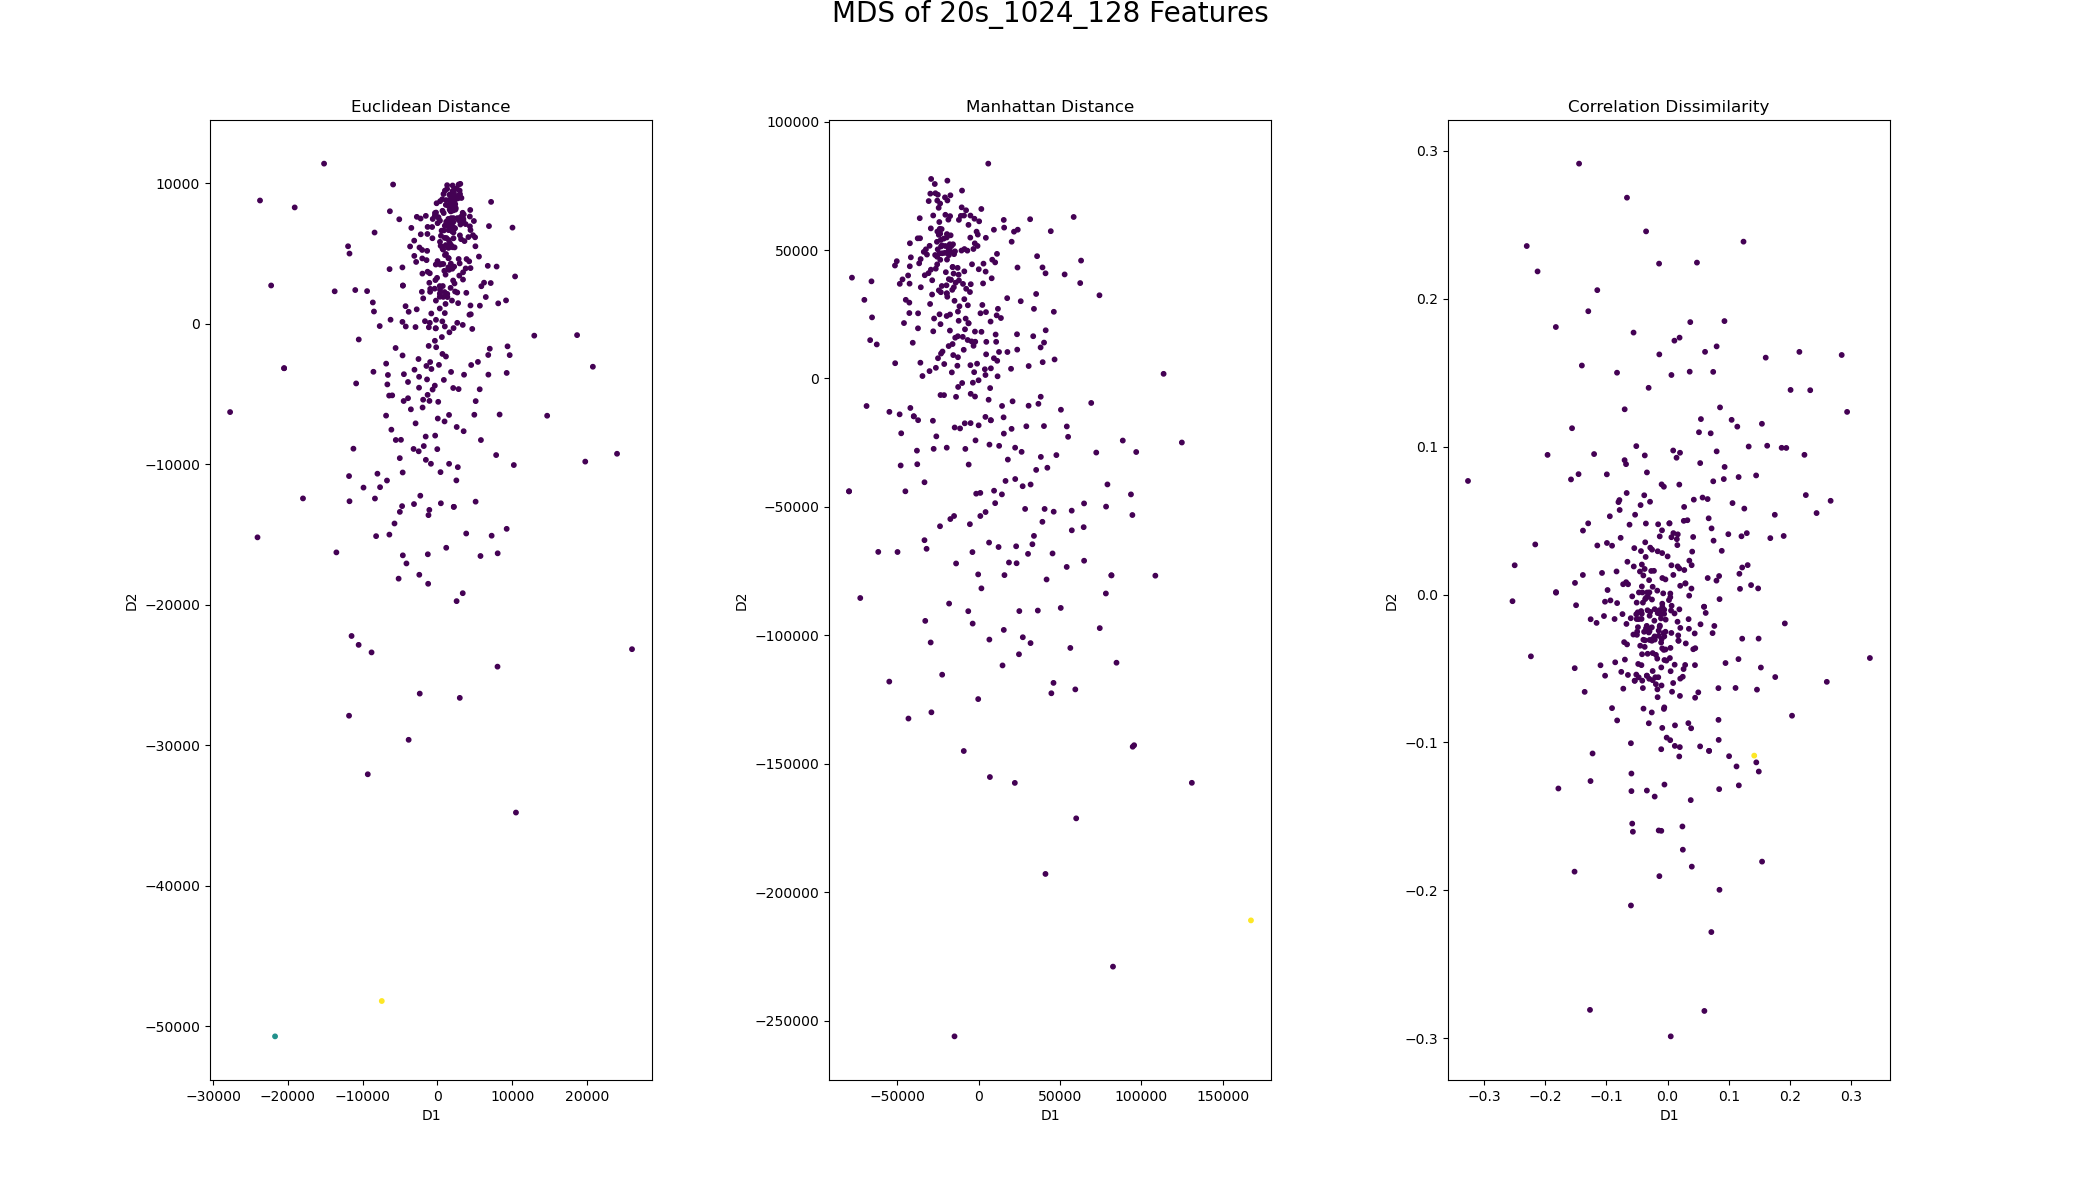
\includegraphics[width=0.9\linewidth]{../Statistical_Sciences_template/figure/MDS of 20s_1024_128 Features Using Single Linkage.png}
	\caption{The plot is the two-dimensional MDS results of the dataset within 20 seconds, 1024 samples of frame length and 128 samples of hop length.}
	\label{fig:MDS of 20s_1024_256 Features Using Single Linkage}
\end{figure}
\noindent The Figure \ref{fig:MDS of 20s_1024_256 Features Using Single Linkage} above is a typical result within single linkage. We can see from the figure that all clustering results are imbalanced: the vast majority of observations form one cluster, while the other cluster is only consisted of one point. This result has no practical significance other than finding that the observation of cluster composed of single points is far away from most observations. This also directly indicates that in high-dimensional spaces, especially in the case of $p>>n$, single linkage is very unstable and unsuitable.\\
\\
\begin{figure}[h!]
	\centering
	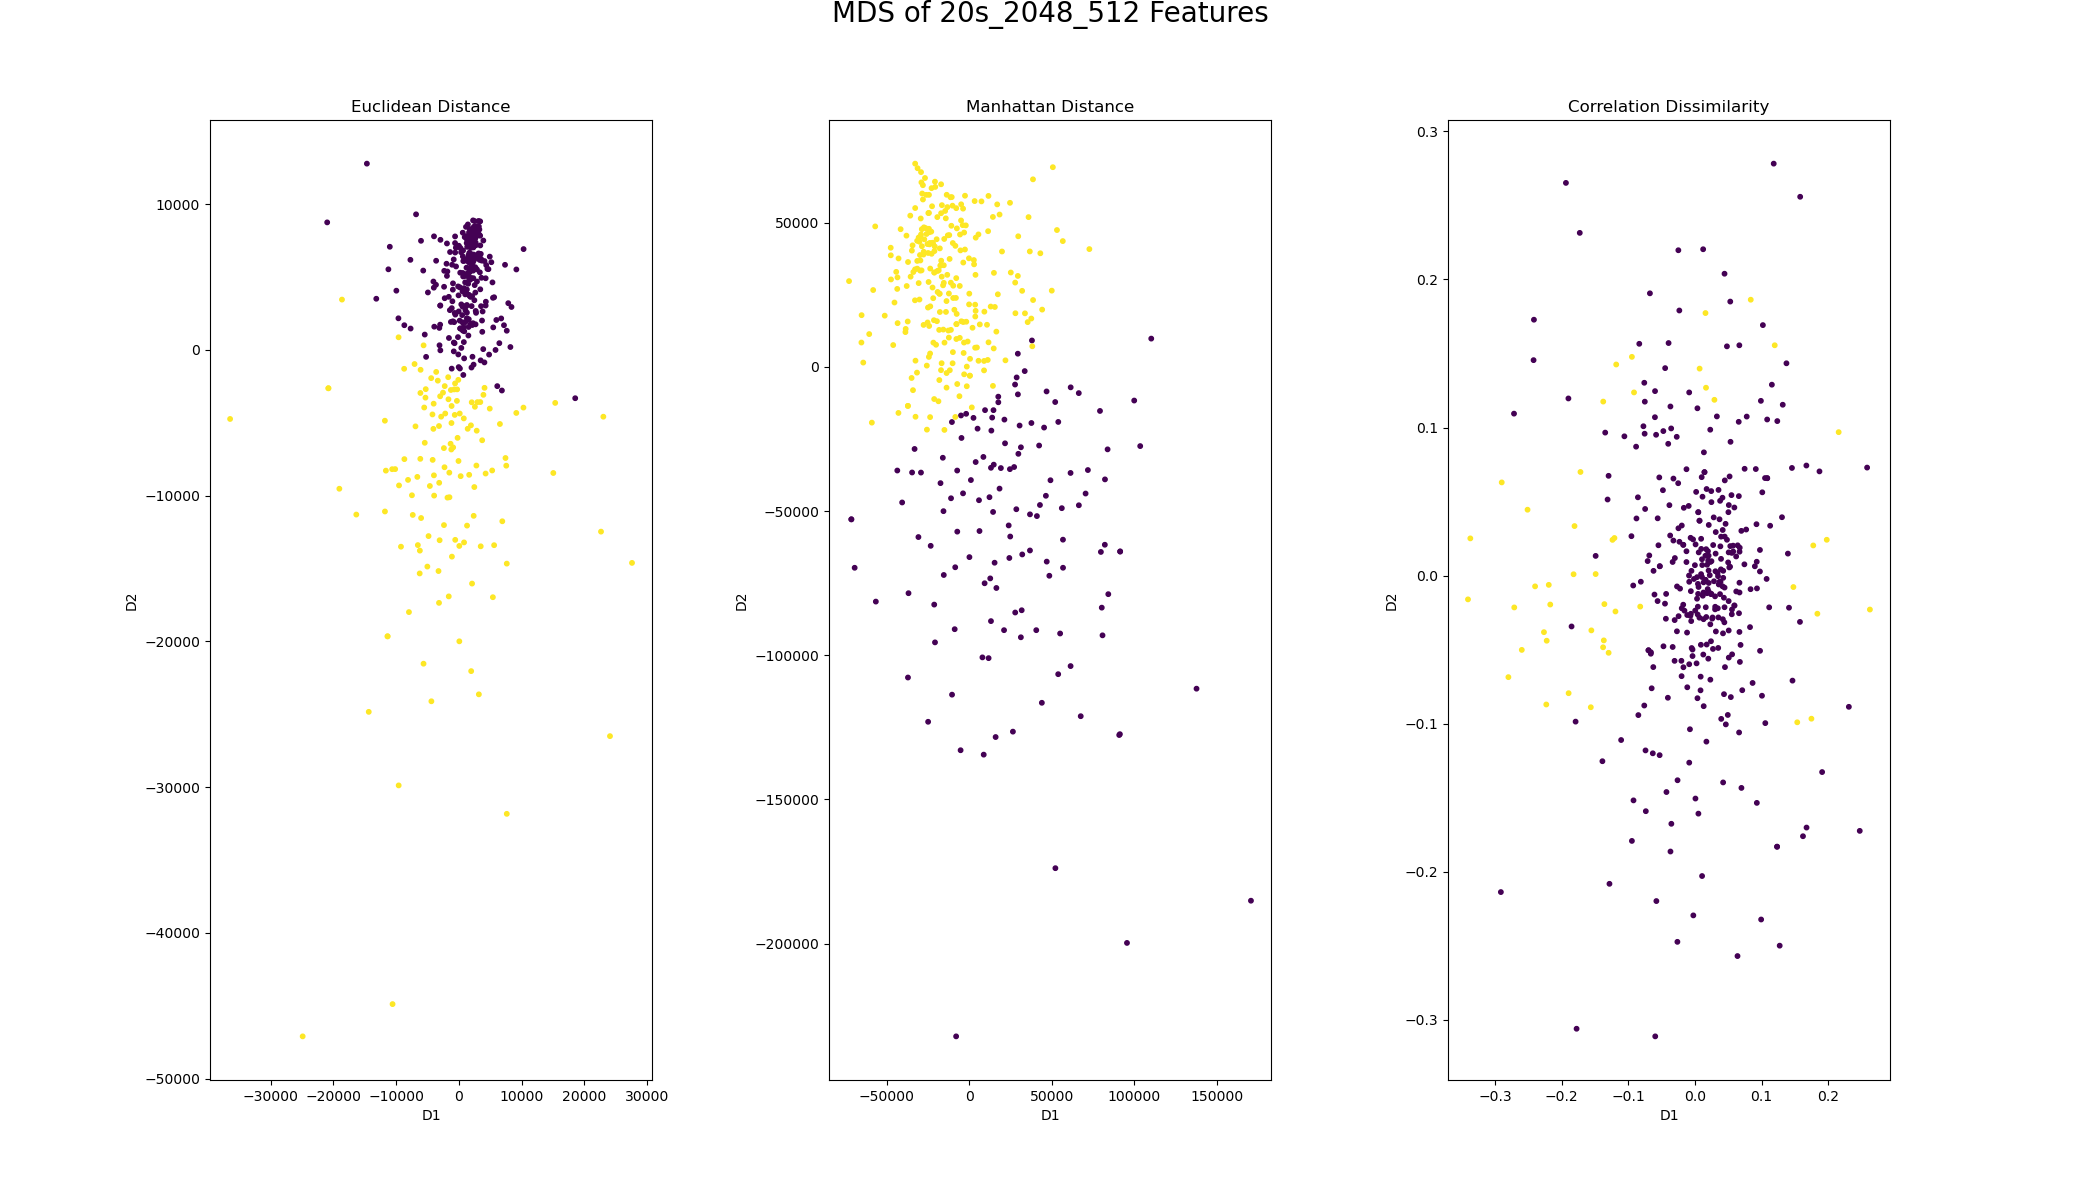
\includegraphics[width=0.9\linewidth]{../Statistical_Sciences_template/figure/MDS of 20s_2048_512 Features Using PAM.png}
	\caption{The plot is the two-dimensional MDS results of the dataset within 20 seconds, 2048 samples of frame length and 512 samples of hop length.}
	\label{fig:MDS of 20s_1024_256 Features Using PAM}
\end{figure}
\noindent The results of PAM clustering are shown in Figure \ref{fig:MDS of 20s_1024_256 Features Using PAM} and are highly consistent with the hierarchical clustering using Manhattan distance combined with complete linkage method. Through the evaluation of ASW, both methods determine that the optimal number of clusters is 2. In the visualization results, the distribution of different clusters is also represented by purple and yellow respectively. The purple cluster shows significant feature homogeneity, and its sample points are closely clustered in the feature space, indicating that these music segments have high similarity in MFCC statistical features. The yellow cluster shows a relatively sparse distribution pattern, suggesting that there is greater variability in the acoustic characteristics of the cluster samples. It is worth noting that although the optimal number of clusters is the same, the boundary of PAM clustering may be clearer than that of hierarchical clustering, which provides a supplementary explanation for subsequent classification tasks such as distance based KNN.\\
\\
\begin{figure}[h!]
	\centering
	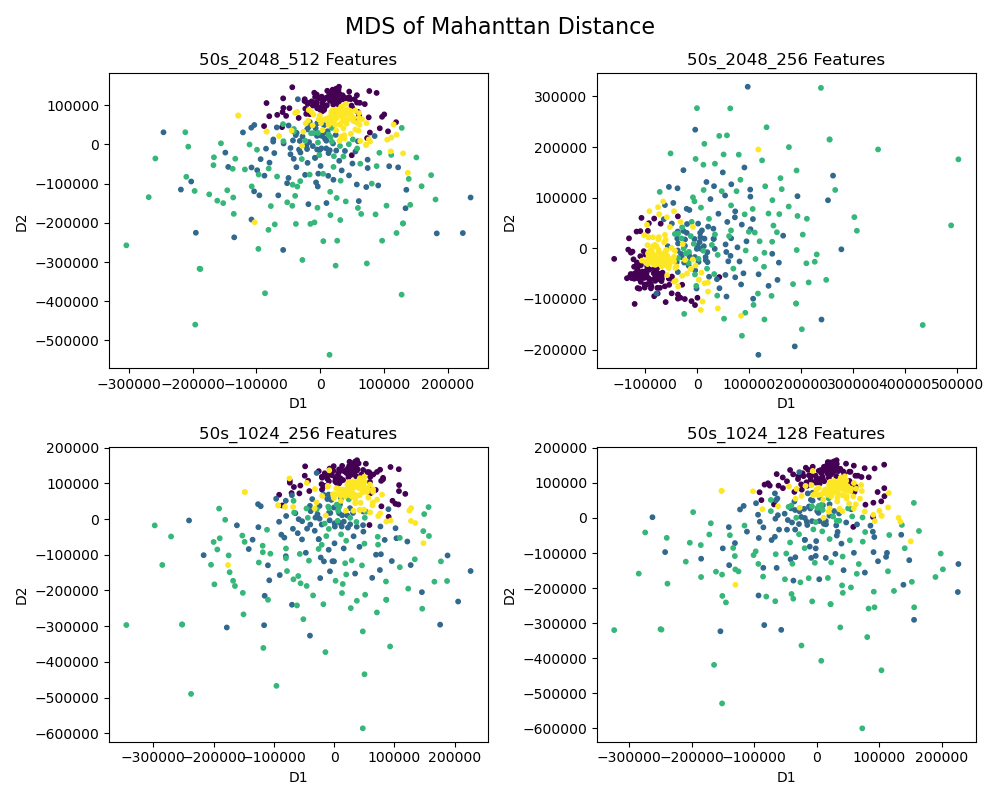
\includegraphics[width=0.9\linewidth]{../Statistical_Sciences_template/figure/MDS of Mahanttan Distance 50s.png}
	\caption{This figure is the MDS visualization of Manhattan distances for the four datasets of 50 seconds}
	\label{fig:MDS of Mahanttan Distance 50s}
\end{figure}
\noindent Unfortunately, these statistical features based on MFCCs cannot clearly reflect the true classification of music genres. From the visualization results in Figure \ref{fig:MDS of Mahanttan Distance 50s} and Figure \ref{fig:MDS of Correlation Dissimilarity 50s}, it can be observed that the acoustic characteristics of different schools show complex distribution patterns in the feature space. In Figure \ref{fig:MDS of Mahanttan Distance 50s}, the purple observation points representing classical music are highly concentrated in the core area with the highest density, while the adjacent yellow observation points (corresponding to disco music) are very close in the feature space, showing amazing similarity. It's worth to note that the blue-green and green observation points representing hiphop and metal music respectively are not only relatively scattered, but also show an obvious crisscross state, which can hardly be effectively distinguished through the boundary. The MDS dimension reduction results in Figure \ref{fig:MDS of Correlation Dissimilarity 50s} also confirm similar findings: although purple observation points (classical music) are distributed at the upper and lower ends of the graph due to the directionality generated by the dimension reduction algorithm (the difference in direction does not change the topology between observations), their overall dispersion is high. The yellow observation point (disco) is still located in the transition area between purple and other observation points. The blue-green and green observations (hiphop and metal) are more mixed.\\
\\
\begin{figure}[h!]
	\centering
	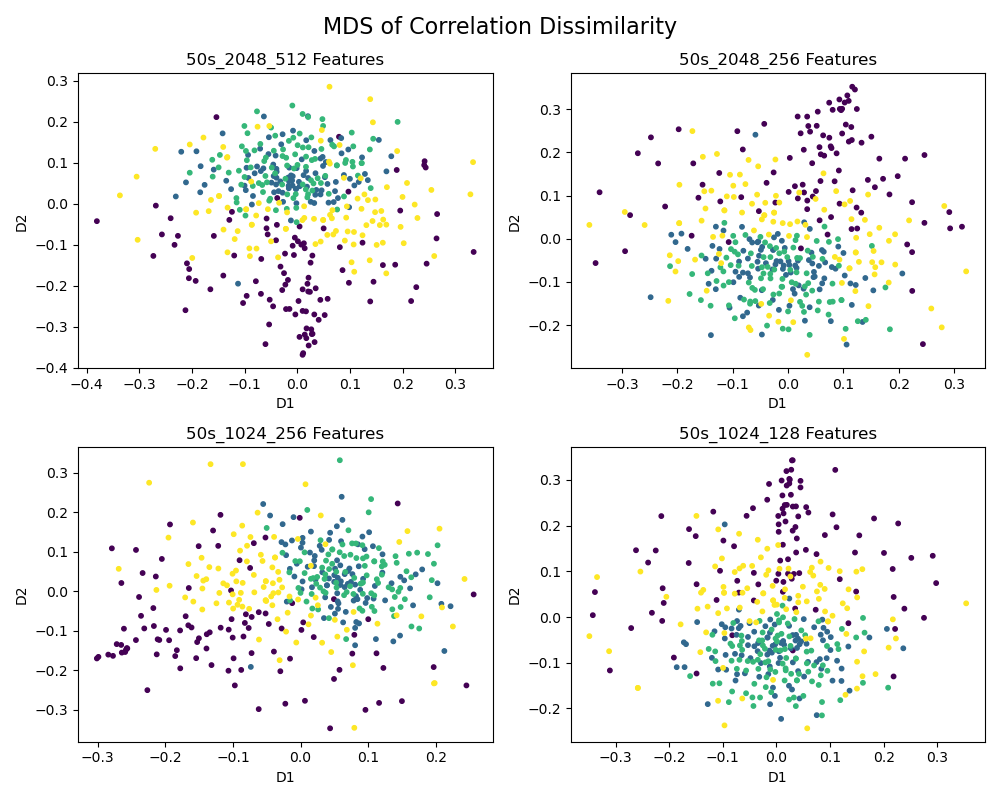
\includegraphics[width=0.9\linewidth]{../Statistical_Sciences_template/figure/MDS of Correlation Dissimilarity 50s.png}
	\caption{This figure is the MDS visualization of correlation dissimilarity for the four datasets of 50 seconds}
	\label{fig:MDS of Correlation Dissimilarity 50s}
\end{figure}
\section{Supervised Statistical Models for Classification}
This section focuses on the complete steps of fitting a supervised learning models based on MFCC statistical features, including model building strategies and specific implementation steps, and evaluates the model performance. In particular, the study focuses on the performance differences between traditional machine learning methods and shapelet tree-based algorithms in music genre classification. In the comparative analysis, we focus on the differences between the two methods in feature representation and classification performance.\\
\\
In terms of the data set partitioning strategy, this study adopts a special processing method that is different from canonical machine learning practices. Considering that the total research data is 400 observations, of which classical, disco, hiphop and mental each accounts for 100. Based on the characteristics of the algorithm and the limitation of computing resources, the data partitioning scheme I designed is as follows: first, 200 samples (accounting for 50\% of the total) are randomly selected from the overall dataset as the training set, then 100 samples (25\%) are randomly selected for the validation set of model parameter tuning, and finally the remaining 100 samples (25\%) are used as the test set to evaluate the final performance of the model.\\
\\
This unconventional data partitioning strategy is mainly due to the inherent limitations of the shapelet tree-based algorithm in terms of computational efficiency. As described in Section \ref{subsec:limit}, the algorithm exhibits a high computational complexity when processing sequence data, and its time complexity reaches $O(\bar{l}^3n^2)$ level, and it needs to evaluate $\sum_{i=1}^n\sum_{j=3}^{l_i-1} j$ candidate shapelets. This computing characteristic leads to two significant problems: first, there will be a serious memory bottleneck during the model fitting process, which is difficult to avoid even in an environment equipped with high-performance computing hardware; second, because the algorithm itself contains a recursive structure, even with GPU acceleration, the model training process is still very slow. Based on these constraints, in order to achieve a feasible model under limited computing resources, I had to control the size of the training set to 50\% of the total data volume. Although this compromise sacrificed some training sample volume, it effectively guaranteed the practicality of the experiment and the research progress.\\
\\

\begin{figure}[h!]
	\centering
	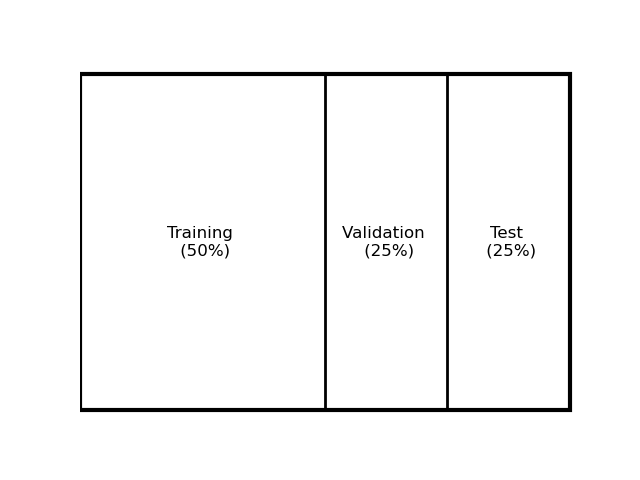
\includegraphics[width=0.9\linewidth]{../Statistical_Sciences_template/figure/Splitting Dataset.png}
	\caption{This is an illustration of how the data set is divided. The training set accounts for 50\% of the total data, the validation set accounts for 25\% of the total data, and the test set also accounts for 25\% of the total data.}
	\label{fig:spliiting}
\end{figure}

\subsection{Fitting the Models}\label{subsec:fitting}
As mentioned in Section \ref{subsec:LR}, Section \ref{subsec:MLR}, Section \ref{subsec:knn} and Section \ref{subsec:SVM} from the previous chapter, this study used methods such as KNN, logistic regression, multinomial logistic regression and support vector machines, and compared the performance of these traditional methods with the results of the shapelet tree-based algorithm. For the traditional statistical learning method, our input is the divided training set mentioned above, and the hyperparameters of various algorithms are tuned through an independent validation set to ensure that each compared model can achieve its optimal performance state, thereby ensuring the reliability of subsequent comparative experiments.\\
\\
Based on the experimental results of Section \ref{subsec:FP}, this study constructed four datasets with different parameters, aiming to explore the key parameter optimization issues in the MFCCs feature extraction process. This strategy enables us to explore the influence of the two key parameters, frame length and hop length, on the model performance. Among them, the choice of frame length directly determines the temporal resolution of time-frequency analysis, while the hop length controls the overlapping part between frames. The optimal combination of these two parameters plays a decisive role in improving the representation ability of speech features. Considering the scale difference problem of the statistical features extracted from MFCC, I adopted a z-score-based normalization method for each variable, which is calculated as 
$$z=\frac{x-\hat{m}}{\hat{s}}$$, 
where $\hat{m}$ represents the sample mean of the feature and $\hat{s}$ represents the sample standard deviation. This normalization process can not only eliminate the dimensional differences between different feature dimensions, but also effectively improve the convergence speed and generalization performance of the model. In order to comprehensively evaluate the influence of data normalization on model performance, I used the standardized MFCCs statistical features for model training on the one hand, and retained the original unstandardized features on the other hand. Thus only the 1-second-long datasets were used for training the model because their dimensions are much lower than that of the 0.4-second-long datasets.\\
\\
When training the KNN classification models, this study examined three different distance metrics, including cosine distance, Manhattan distance, and Euclidean distance. It should be noted that when using cosine distance as a metric, we only used the original statistical feature data that was not standardized for model training, and did not fit a KNN model based on cosine distance for the standardized data. The theoretical basis of this strategy is that z-score standardization, as a linear transformation method, only translates and scales the original data vectors without changing the relative direction relationship of the vectors in the feature space. Since the calculation of cosine distances essentially reflects the cosine values of the angle between vectors, its calculation result is only related to the direction of the vectors, and after L2 norm normalization, the influence of vector length has been completely eliminated. Therefore, standardization does not change the similarity measurement result based on cosine distance, which makes it unnecessary to train a KNN model based on cosine distance after standardization.\\
\\
Based on the above analysis, this experiment adopted the following modeling strategy: for the unstandardized original statistical feature data, we trained a KNN model containing all three distance metrics (cosine distance, Manhattan distance and Euclidean distance); for the standardized data, only the KNN model based on Manhattan distance and Euclidean distance was fitting. Considering that KNN is a typical nonparametric statistical learning method, its model performance mainly depends on the selection of the key hyperparameter $K$, the number of neighbors. Therefore, we adopted a systematic parameter optimization method: in the experiment, we tested integer values of $K$ from 2 to 10, trained the corresponding KNN model for each candidate K value, and evaluated its performance by calculating the classification accuracy of the model on the validation set. Finally, we selected the K value corresponding to the highest classification accuracy on the validation set as the optimal hyperparameter of the model.\\
\\
\\
\\
In the process of training logistic regression and multinomial logistic regression models, this study uniformly adopted L1 penalty for high dimensional data where the number of training set observations $n$ is significantly less than the number of feature variables $p$ (i.e. $n<<p$). This method is chosen because: when the feature dimension $p$ is much larger than the sample size $n$, if the classical maximum likelihood estimation method is directly used for parameter estimation (as described in Section \ref{subsec:LR} and Section \ref{subsec:MLR}), some problems for matrix computation will occur. Specifically, the maximum column rank of the design matrix $X$ is $n$. When $p>n$, the matrix $X^TX$ must be irreversible, resulting in the covariance matrix of the parameter estimation being non positive definite. At this time, there are more than one combinations of regression coefficients that can simultaneously reach the maximum value of the likelihood function or the minimum value of the loss function. From a geometric perspective, the sparsity of data points in high dimensional feature space leads to the existence of multiple hyperplanes that meet the linear separability condition, which directly leads to no unique model solutions. In addition, during the maximum likelihood estimation process, the algorithm can easily pursue the maximization of the likelihood function by making the some regression coefficients corresponding to specific features be infinity, which not only leads to the instability of numerical calculations, but also significantly reduces the parameter convergence speed and even causes divergence.\\
\\
The core advantages of introducing L1 penalty (lasso penalty) are reflected in three aspects: first, by applying L1 penalty, the regression coefficients of some unimportant features are shrunk to zero exactly, thereby achieving feature selection, which is of great value for eliminating redundant features and improving model interpretability; second, the geometric characteristics of L1 penalty (the vertices of the diamond constraint domain are located on the coordinate axis) can effectively compress the size of solution space, and in most cases, many solutions can be converted into a finite number of sparse solutions, and even in some cases, the only optimal solution can be obtained. It should be noted that when there are completely collinear features (such as two completely correlated variables), although L1 penalty cannot completely find the unique solution (it may randomly retain one of the features and discard the other), its solution space dimension has been greatly reduced compared to the original model without any constraints, which still has significant advantages in practical applications. This experiment did not conduct a deep discussion on this extreme case, mainly because the probability of complete collinearity in reality is low.\\
\\
In comparison, although L2 penalty (ridge penalty) can mathematically ensure that parameter estimation has a unique solution, its core disadvantage is that it cannot achieve feature selection——all regression coefficients are proportionally compressed through quadratic penalty terms, resulting in a large number of redundant or noise features still being retained in the model, which not only reduces the interpretability of the model, but may also cause additional variance due to the unimportant noise features. In addition, there are fundamental limitations in the way L2 penalty dealing with collinearity problems: when highly correlated feature groups exist, it tends to retain the regression coefficients of each corresponding variable rather than perform feature selection. More importantly, L2 penalty cannot effectively eliminate the numerical calculation difficulties caused by matrix singularity in high dimensional data, where the model convergence speed may still be seriously affected. Therefore, L2 or elastic net, which includes the L2 penalty term, was not used in this experiment.\\
\\
Another point to note is that in the process of statistical modeling, the selection of regularization parameters has a decisive influence on the performance of the logistic regression model and the multinomial logistic regression model. In other words, the setting of the L1 regularization parameter $\lambda$ is particularly critical. This parameter directly controls how many coefficients of the model will shrink to 0 exactly. The larger the lambda value, the stronger the penalty imposed on the model coefficients, which will cause more coefficients to shrink to 0, thereby effectively reducing the complexity of the model and preventing the occurrence of overfitting. Conversely, when the lambda value is small, the regularization effect is weakened and the model retains more feature information. In particular, when $\lambda=0$, the model will degenerate into a standard logistic regression or multinomial logistic regression form, and no regularization constraints are imposed at this time. In this study, the optimal lambda value was determined using a statistical method based on the performance of the validation set, that is, the classification accuracy of the model on the validation set under different lambda values was evaluated, and the lambda value that maximized the accuracy of the validation set was finally selected as the optimal parameter. It should be noted that since this study uses Python's scikit-learn library to implement model training, the regularization strength is controlled by the parameter $C$ in the LogisticRegression class. From a mathematical perspective, $C$ is the reciprocal of $\lambda$, that is $C=\frac{1}{\lambda}$. This parameterization means that a larger $C$ value corresponds to a smaller regularization strength, while a smaller C value corresponds to a stronger regularization effect.\\
\\
\\
\\
The last traditional statistical learning method used in this study is the Support Vector Machine (SVM), specifically the Linear Support Vector Classifier. In the process of model selection, I experimented with the applicability of various kernel functions, including nonlinear kernel functions such as the Polynomial Kernel and the Gaussian Kernel. However, due to the typical high dimensional features of the data in this study (i.e., the feature dimension p is much larger than the sample size n), the nonlinear kernel function showed a significant overfitting tendency during the training process, and its classification performance was significantly inferior to that of the linear kernel function. Based on the quantitative comparison of the validation results, I finally decided to use only the linear kernel function for subsequent analysis.\\
\\
Considering that each feature variable in the high dimensional data has different scales and distribution ranges, directly using the original data for modeling may cause the optimization algorithm to fail to converge, and also make the model have an unreasonable preference for features with larger dimensions. For this reason, I tried to use the standardized data for model training and subsequent analysis and comparison instead of using the original data. Similar to the logistic regression and multinomial logistic regression models used in this study, the linear support vector classifier also introduces the L1 penalty to reduce the risk of overfitting and enhance the robustness of the model.\\
\\
In terms of the technical details of the model implementation, it should be noted that the linear support vector classifier used in this study is implemented based on the LinearSVC class of the scikit-learn machine learning library in the Python. The algorithm implementation of this class is derived from the LIBLINEAR efficient optimization library developed by Fan et al. (2008). In this article, the loss of the support vector machine is defined as follows:
$$
\min_{\mathbf{w}}\frac{1}{2} \mathbf{w}^T\mathbf{w}+C\sum\xi(\mathbf{w},\mathbf{x},y),
$$
which is corresponding to Equation \eqref{svmL2}. The term "L1-SVM" proposed by Fan et al. in their original paper specifically refers to the support vector machine model using the standard hinge loss function (i.e., L1 loss), that is
$$
\max(1-y\mathbf{w}^T\mathbf{x},0),
$$
which is essentially different from the model used in this study. Although the model actually used in this study also applies the L1 regularization penalty term, its loss function adopts the form of squared hinge (L2 loss), that is
$$
\max(1-y\mathbf{w}^T\mathbf{x},0)^2
$$
In summary, there are two major differences between L1-SVM and the model in this study: one is the penalty term, which is the L2 norm in L1-SVM and the L1 norm in this model; the other is the part of loss function, which is the hinge loss in L1-SVM and the squared hinge loss in this model. Accordingly, the corresponding loss for the model in my study is Equation \eqref{svmL1}, while the loss for L1-SVM corresponds to \eqref{svmL2}.\\
\\
\\
\\
The implementation of the shapelet algorithm in this study uses a completely different technical route from the traditional statistical model method. In the early exploration stage, I first tried to reduce the dimensionality of the original audio signal. Specifically, I used an operation method similar to pooling, that is, to segment the audio signal, extract audio segments of fixed length (including 1 second and 0.4 second duration settings), and then calculate two statistical features of each segment: maximum value (max pooling) and mean (mean pooling). This statistical feature based sequence compression method aims to convert the high-dimensional original audio signal into a low dimensional time series representation, thereby meeting the shapelet algorithm's requirements for the input data dimension.\\
\\
However, after multiple experimental verifications, this strategy showed serious problems in multiple key indicators. During the model training process, when a deeper decision tree structure was used, the model performed well on the training set, with an accuracy generally above 0.7, but the performance on the validation set and test set dropped sharply, with the accuracy mostly less than 0.3, and some models even as low as around 0.2. This huge performance gap indicates that the model has a serious overfitting problem. To improve this situation, I tried to reduce the model complexity (that is, reduce the depth of the tree) by adjusting the model parameters, and also tried to increase the sample size of the training set. Although these adjustments did alleviate the overfitting phenomenon, they led to new problems-the model began to show obvious underfitting characteristics, and the accuracy on the training set, validation set, and test set remained at a low level.\\
\\
This dilemma could not be effectively resolved after many attempts at parameter tuning. Specifically, when trying to find an intermediate parameter setting, the model either still has a certain degree of overfitting or tends to underfit. I realized that this dimensionality reduction strategy based on pooling operations is inherently in conflict with the characteristics of the shapelet algorithm. The shapelet algorithm needs to identify key local subsequence features in the time series, and the shapelets found after the pooling operation are not representative enough. This information loss makes it difficult for the algorithm to find truly discriminative shapelets, which ultimately leads to the complete abandonment of the strategy.\\
\\
Another important idea proposed in this study comes from the observation and analysis of MFCCs features. Through the change patterns of MFCCs coefficients shown in Figure \ref{fig:Low MFCCs} and Figure \ref{fig:High MFCCs}, we found that low-frequency cepstral coefficients (especially the first MFCCs) showed significant differences in the time dimension, while high-frequency cepstral coefficients showed a highly consistent change trend. This obvious difference in spectral characteristics prompted us to form a key hypothesis: low-frequency cepstral coefficients are likely to contain the most representative shapelet patterns due to their more significant temporal variation characteristics and stronger discrimination. Based on this important discovery, I decided to use the mean sequence of the first MFCCs as the basic data for model training. The specific implementation method is as follows: in the feature engineering processing stage, I calculated the mean of 50 first MFCCs for each 0.4 second analysis window, and these processed mean sequences constituted the core input data for subsequent shapelet model training. That is to say, in the results of feature project in Section \ref{subsec:FP}, the mean of the MFCCs data of the corresponding 0.4 second analysis window is used to train the model. Because the audio data is sampled from the 5th second for 20 seconds, each observation has a length of 20 seconds, so this feature project will generate a feature time series of length 50, and the training of the shapelet tree-based algorithm model is based on these sequences of length 50. This modeling strategy based on specific frequency band features not only retains the most discriminative temporal feature information, but also achieves reasonable data dimensionality reduction through mean processing.\\
\\
\subsection{Results and Performance}\label{subsec:performance}
After all models were trained with the training set and the validation set parameters were optimized, the results are shown in the following table. In the table, std represents the standardized data, the first number represents the frame length, and the second number represents the hop length.\\
\\
Table \ref{table:KNN} shows in detail the classification performance of the dataset after feature project and its standardized version on the test set after training using KNN algorithm. First, as mentioned in the beginning of Section \ref{subsec:fitting}, the calculation results of cosine distance are not affected by data standardization due to its inherent scale invariance, so the results of the standardized dataset are not shown Table \ref{table:KNN}.\\
\begin{table}[H]
	\centering
	\caption{Performances of KNN Algorithm}
	\begin{tabularx}{\linewidth}{>{\raggedright\arraybackslash}X *{3}{>{\centering\arraybackslash}m{3.5cm}}}
		\toprule
		Data Set     & KNN with Cosine & KNN with Euclidean & KNN with Manhattan  \\ \midrule
		2048 512     & 0.48            & 0.61               & 0.75                              \\
		2048 256     & 0.52            & 0.65               & 0.72                              \\	
		1024 256     & 0.50            & 0.57               & 0.76                              \\	
		1024 128     & \textbf{0.43}   & 0.56               & 0.77                              \\
		std 2048 512 &             & 0.77                   & 0.8                              \\
		std 2048 256 &             & 0.8                    & 0.8                              \\	
		std 1024 256 &             & 0.82                   & 0.87                              \\	
		std 1024 128 &             & 0.8                    & 0.83                              \\ \bottomrule
	\end{tabularx}
	\label{table:KNN}
\end{table}

\noindent In terms of specific performance, the experimental results of the KNN model show significant differences. When the dataset with 1024 samples of frame length and 128 hop length is applied within the cosine distance metric, the model performs the worst, with a test set accuracy of only 0.43, which is significantly lower than the model performance under other configuration conditions. In sharp contrast, when the standardized dataset with 1024 samples of frame length and 256 hop length is applied the Manhattan distance metric, the model performs the best of all KNN models, with a test set accuracy of 0.87, which is nearly double the worst configuration.\\
\\
By comparing and analyzing the datasets with different parameter configurations, the following important findings can be drawn: first, the parameter differences of frame length and hop length have relatively limited influence on the performance of the KNN model, in other words, the performance of the models under different parameter configurations of feature project is not much different. For example, the test set accuracy of the standardized data set in the KNN model based on Manhattan distance is more than 0.8, and the test set accuracy of the unstandardized data set in the KNN model based on Euclidean distance is also around 0.61. The differences between them are not obvious. However, it is worth noting that data standardization has a significant effect on improving model performance. Specifically, whether Euclidean distance or Manhattan distance is used as the distance metric, the standardized data set can bring significant accuracy improvement, and this phenomenon has been verified in all the datasets. Further analysis of the performance differences of different distance metrics can reveal a stable and significant rule: under the condition of fixed frame length and hop length, the performance of the distance metric shows obvious gradient differences, with Manhattan distance performing the best, Euclidean distance second, and cosine distance performing the worst. In addition, experimental results also show that the choice of distance metric influence model performance even more than the choice of feature project parameters.\\
\\
Table \ref{table:L1penalty} shows the performance comparison of three classical classification models using L1 penalty constraints, including logistic regression, multinomial logistic regression, and SVM (linear support vector classifier), on the unstandardized dataset and the standardized dataset. It should be noted that due to the serious convergence problem when training the linear support vector classifier on the unstandardized dataset (no matter how many iterations were taken), the test results under this condition are not reliable, so they are not presented in the table. In addition, although the traditional logistic regression is mainly applicable to binary classification scenarios, this study uses the "one-vs-rest" strategy to construct a combination of four independent logistic regression models, thereby achieving multi-classification capabilities. This strategy can be easily achieved by the scikit-learn class LogisticRegression() within the solver "liblinear" in Python, which is also a part of the work by Fan et al. (2008).\\

\begin{table}[H]
	\centering
	\caption{Performances of Algorithms with L1 Penalty}
    \begin{tabularx}{\linewidth}{>{\raggedright\arraybackslash}X *{3}{>{\centering\arraybackslash}m{3.5cm}}}
	\toprule
Data Set     &  LR & Multinomial LR & Linear SVM  \\ \midrule
2048 512     & 0.74       & 0.65            &                                            \\
2048 256     & 0.77       & 0.65            &                                            \\	
1024 256     & 0.78       & 0.6            &                                            \\	
1024 128     & 0.73       & 0.65            &                                            \\
std 2048 512 & 0.72       & 0.82            & 0.83                                            \\
std 2048 256 & 0.67       & 0.86            & 0.82                                           \\	
std 1024 256 & 0.67       & \textbf{0.89}             & 0.81                                           \\	
std 1024 128 & 0.67        & \textbf{0.89}           & 0.86                                           \\ \bottomrule
	\end{tabularx}
	\label{table:L1penalty}
\end{table}

\noindent Several important findings can be drawn from the experimental results. First, the impact of data standardization on model performance shows obvious differences. The standardized data set showed excellent classification performance on both the multinomial logistic regression and SVM models, and the test set accuracy exceeded 0.8. It is particularly noteworthy that the standardized data set with 1024 frame length and 128 jump length combined with the multinomial logistic regression model achieved the best classification effect, with a test accuracy of 0.89. Analyzing the impact of standardization on different models, we found an interesting phenomenon: standardization caused the performance of the logistic regression combination model to decline (an average decrease of about 0.07), but significantly improved the accuracy of the multinomial logistic regression model (an average increase of about 0.2).\\
\\
In the performance comparison of different models, we observed the following pattern: for the standardized data set, the performance of the logistic regression combination is better than that of the multinomial logistic regression, with the test accuracy of the former being stable at above 0.73, while the latter is concentrated at 0.65. However, on the standardized data set, this superiority-inferiority relationship is reversed: the accuracy of the multinomial logistic regression is over 0.82, significantly higher than the highest accuracy of 0.72 of the logistic regression combination. The standardization process effectively eliminates the performance bottleneck of the multinomial logistic regression. It is worth noting that under standardized conditions, the performance of the multinomial logistic regression and the linear support vector classifier is quite close, with the accuracy difference between the two not exceeding 0.04, and the performance of the two on the test set is alternately leading. Based on the experimental results above, we can draw the following conclusions: under the conditions of standardized data, the performance of the three models presents a hierarchical structure. Logistic regression performs the worst, while multinomial logistic regression and SVM models show similar and significantly superior performance.\\
\\
Table \ref{table:best} shows the evaluation results of the best model, i.e. the multinomial logistic regression trained on the standardized dataset with 1024 frame length and 128 hop length, on the test set, covering all four categories (classical, disco, hiphop, and mental), as well as the overall macro-average and weighted average evaluation scores. From the results, the model performs best on classical, with precision, recall, and F1-score all reaching 1.00, indicating that the model can correctly identify all samples in this category without misclassification or omission. The performance of hiphop is also relatively stable, with all three indicators being 0.89, indicating that the model has a relatively balanced classification effect on it. In contrast, there are some fluctuations in the indicators of disco and mental: the precision of disco is high (0.95), but the recall rate is a little bit lower (0.72), which means that nearly 28\% of the samples of this category are missed by the model, and the shortcoming of the recall lowers the F1-score. While mental is the opposite, with a recall rate of 0.95, indicating that the model has a strong coverage of this category, but the precision rate is only 0.75, which may misclassify other categories as this category, resulting in more false positives. Overall, the macro average and weighted average F1-scores of the model are both 0.89, which is the harmonic average of precision and recall, indicating that the overall performance is relatively stable and there is no obvious deviation due to the difference in the number of samples (the support number of each category is between 22 and 27).\\

\begin{table}[H]
	\centering
	\caption{Performance of Multinomial LR within Standard 1024 128 Dataset}
	\begin{tabularx}{\linewidth}{>{\raggedright\arraybackslash}X *{4}{>{\centering\arraybackslash}m{2.8cm}}}
		\toprule
		&  Precision & Recall & F1-score & Support \\ \midrule
		Classical     &  1.00  & 1.00  & 1.00  &  26    \\
		Disco     &  0.95  & 0.72  & 0.82  &  25  \\
		Hiphop     &  0.89  & 0.89  & 0.89  &  27   \\
		Mental     &  0.75  & 0.95  & 0.84  &  22   \\
		\\
		macro avg  & 0.90 & 0.89 &0.89 & 100 \\
		weighted avg  & 0.90 & 0.89 &0.89 & 100 \\  \bottomrule
	\end{tabularx}
	\label{table:best}
\end{table}

\noindent Table \ref{table:shapeletmodels} shows the classification accuracy of the shapelet tree-based algorithm on the test set. Compared with the traditional statistical learning methods such as multinomial logistic regression and SVM models mentioned above, the classification performance of this algorithm is relatively weak. The best model trained on the dataset within 2048 frame length and 256 hop length only achieved an accuracy of 0.63. Although this value is significantly lower than the classification results of some other models, the result is significantly different from the null model (random guessing) and is a little better than that of the KNN models using cosine distance, indicating that the algorithm does have a certain degree of discrimination ability. A detailed analysis and discussion of the performance limitations of this algorithm will be carried out in Section \ref{subsec:explaination}, including a comparative study with other algorithms and a discussion of potential improvement directions.\\


\begin{table}[H]
	\centering
	\caption{Performances of Shapelet Tree-based Algorithm}
	\begin{tabularx}{\linewidth}{>{\raggedright\arraybackslash}X *{4}{>{\centering\arraybackslash}m{3cm}}}
		\toprule
		Data Set     &  2048 512 & 2048 256 & 1024 256 & 1024 128 \\ \midrule
		Accuracy     & 0.55      & 0.63     & 0.51     & 0.53    \\ \bottomrule
	\end{tabularx}
	\label{table:shapeletmodels}
\end{table}

\noindent Table \ref{table:bestshapelet} shows the multi-classification performance evaluation results of the shapelet tree-based algorithm on the dataset within 2048 frame length and 256 hop length. From the comprehensive performance of precision, recall, and F1-Score, the performance of the model in different categories varies significantly, and the overall performance is moderate. The macro average and weighted average are both 0.63 to 0.64, indicating that the model's capabilities need to be improved.\\
\\
Classical performs best, with a precision of 1.00, which means that all samples predicted by the model as classical do belong to this category without misclassification. However, its recall rate is 0.85, indicating that 15\% of classical samples are still misclassified into other categories, probably because the features of these samples partially overlap with other music types. Despite this, classical's F1-score is 0.92, the highest among the four categories, reflecting the high reliability of its prediction results. In contrast, disco performed the worst, with a precision of only 0.47, indicating that the model had a high misclassification rate when predicting disco, and more than half of the predictions may be wrong. At the same time, its recall rate was as low as 0.32, which means that 68\% of Disco samples were not correctly identified. This combination of low precision and low recall resulted in an F1-score of only 0.38 for disco, indicating that the model had serious difficulties in identifying this category.\\

\begin{table}[H]
	\centering
	\caption{Performances of Shapelet within 2048 256 Dataset}
	\begin{tabularx}{\linewidth}{>{\raggedright\arraybackslash}X *{4}{>{\centering\arraybackslash}m{2.8cm}}}
		\toprule
		&  Precision & Recall & F1-Score & Support \\ \midrule
		Classical     &  1.00  & 0.85  & 0.92  &  26    \\
		Disco     &  0.47  & 0.32  & 0.38  &  25  \\
		Hiphop     &  0.52  & 0.63  & 0.57  &  27   \\
		Mental     &  0.57  & 0.73  & 0.64  &  22   \\
		\\
		macro avg  & 0.64 & 0.64 &0.63 & 100 \\
		weighted avg  & 0.64 & 0.64 &0.63 & 100 \\ \bottomrule
	\end{tabularx}
	\label{table:bestshapelet}
\end{table}

\noindent The performance of the hiphop and mental categories was at an intermediate level. Hiphop had a precision of 0.52, a recall of 0.63, and an F1 score of 0.57, indicating that the model had average recognition ability for it, with some misclassification and misidentification. It is worth noting that the recall rate of hiphop is higher than the precision rate, indicating that the model tends to classify more samples as hiphop, but nearly half of them may be wrong. The recall rate of the mental is high (0.73), but the precision rate is only 0.57, which means that although the model can capture most of the mental samples, it is also easy to misclassify the samples from other categories as mental, resulting in more false positives. This imbalance makes its F1 score 0.64, which is better than hiphop and disco, but still not ideal.\\
\\
Overall, the macro average and weighted average are both around 0.64, and the support shows that the sample size of each category is relatively balanced (between 22 and 27), indicating that the performance difference of the model is not caused by data imbalance, but is more likely related to the limitations of feature extraction or the algorithm itself. In particular, the significant shortcomings of the disco category drag down the overall performance. Overall, the current model performs well on classical, but there is still much room for improvement in other categories.\\
\\

\subsection{Explainations of the Models}\label{subsec:explaination}
We can see from Table \ref{table:KNN} that among all the KNN model evaluations, the model using Manhattan distance as the metric exhibits the best classification performance on the standard dataset with 1024 frame length and 256 hop length, with a test set accuracy of 0.87, which is higher than the performance of other KNN models. And as described in Section \ref{subsec:performance}, when the model uses L1 distance, regardless of whether the data is standardized, its results on the test set are better than those using Euclidean distance, and this advantage remains consistent under different parameter configurations.\\
\\
This may be because the Manhattan distance is more robust in feature space, especially in high-dimensional space, while the Euclidean distance or other Minkowski distances with p>2 are not as robust as the Manhattan distance because they use exponentiation operations, which easily amplifies the impact of individual extreme observations. As a result, individual observations in high-dimensional space greatly affect the structure of the model.\\
\\
Moreover, when $p>>n$, the sample points are sparse in the feature space, which may cause the Euclidean distance to not be a good measure of the difference between points. Just like the results of clustering using the Euclidean distance in Section \ref{subsec:clustering}, almost all the results are two clusters: one is composed of the vast majority of observations, and the other is only one observation, such as the result of Euclidean clustering in Figure \ref{fig:MDS of 20s_1024_256 Features Using Complete Linkage}. The clustering results can further illustrate from the side that the Euclidean distance has a poor distinction between samples in high-dimensional space. The Euclidean distance between sample points will approach almost the same value, which is difficult to reflect the differences between samples. As a result, similar phenomena lead to poor results of the KNN model under the Euclidean distance. On the contrary, the Manhattan distance has some obvious distinction between samples in the clustering model, and the clustering results are meaningful, such as the Manhattan clustering results in Figure \ref{fig:MDS of 20s_1024_256 Features Using Complete Linkage}. This more discriminating result makes the KNN model using the Manhattan distance perform better than that using the Euclidean distance.\\
\\
Figure \ref{fig:MLRstdcoef} is the heatmap of coefficients of the multinomial logistic regression models trained on the standardized dataset. In this visualization, the white area indicates that the regression coefficient at the corresponding variable is zero, while the color depth is positively correlated with the absolute value of the coefficients. From this heatmap, we can observe that the L1 penalty term does effectively achieve the sparse features of the model coefficients, and the regression coefficients of most variables are compressed to zero exactly. This feature significantly reduces the adverse influence of high dimensional data on model complexity. It is also worth noting that among all the multinomial logistic regression models fitted on standardized data, the model based on the dataset with frame length 2048 and hop length 512 performs relatively poor. From the intuitive presentation of Figure \ref{fig:MLRstdcoef}, we can see that the coefficients' matrix of this dataset presents the most sparse distribution features, while the coefficient distribution of the other three models is more dense. By calculation, we can find that among the four regression models, the proportion of non-zero coefficients of the dataset with frame length 2048 and hop length 512 is about 0.040, while the proportion of non-zero coefficients in the remaining three datasets is about 0.268, which is much higher than that of the first one. This phenomenon provides a reasonable explanation for the difference in model performance: in the dataset with frame length 2048 and hop length 512, due to the great effect of the L1 penalty term, a large number of coefficients are forced to shrink exactly to zero, and these eliminated coefficients actually contain some feature information with predictive value. In other words, the model may have excessively excluded some variables with discriminative ability during the feature selection process, causing a slight underfitting problem. In contrast, the other three models retain more non-zero coefficients and can make more full use of the effective information in the data, thus obtaining relatively better prediction performance. This difference further verifies the trade-off between regularization and model complexity: although a L1 penalty can effectively control model complexity, it may lead to the loss of valuable information; while moderately relaxing the regularization constraint helps to improve the expressive power of the model. In addition, this phenomenon also suggests that the MFCCs of the dataset with frame length 2048 and hop length 512 may have slightly different feature distribution features from other datasets, making it more sensitive to L1 penalty. \\

\begin{figure}[H]
	\centering
	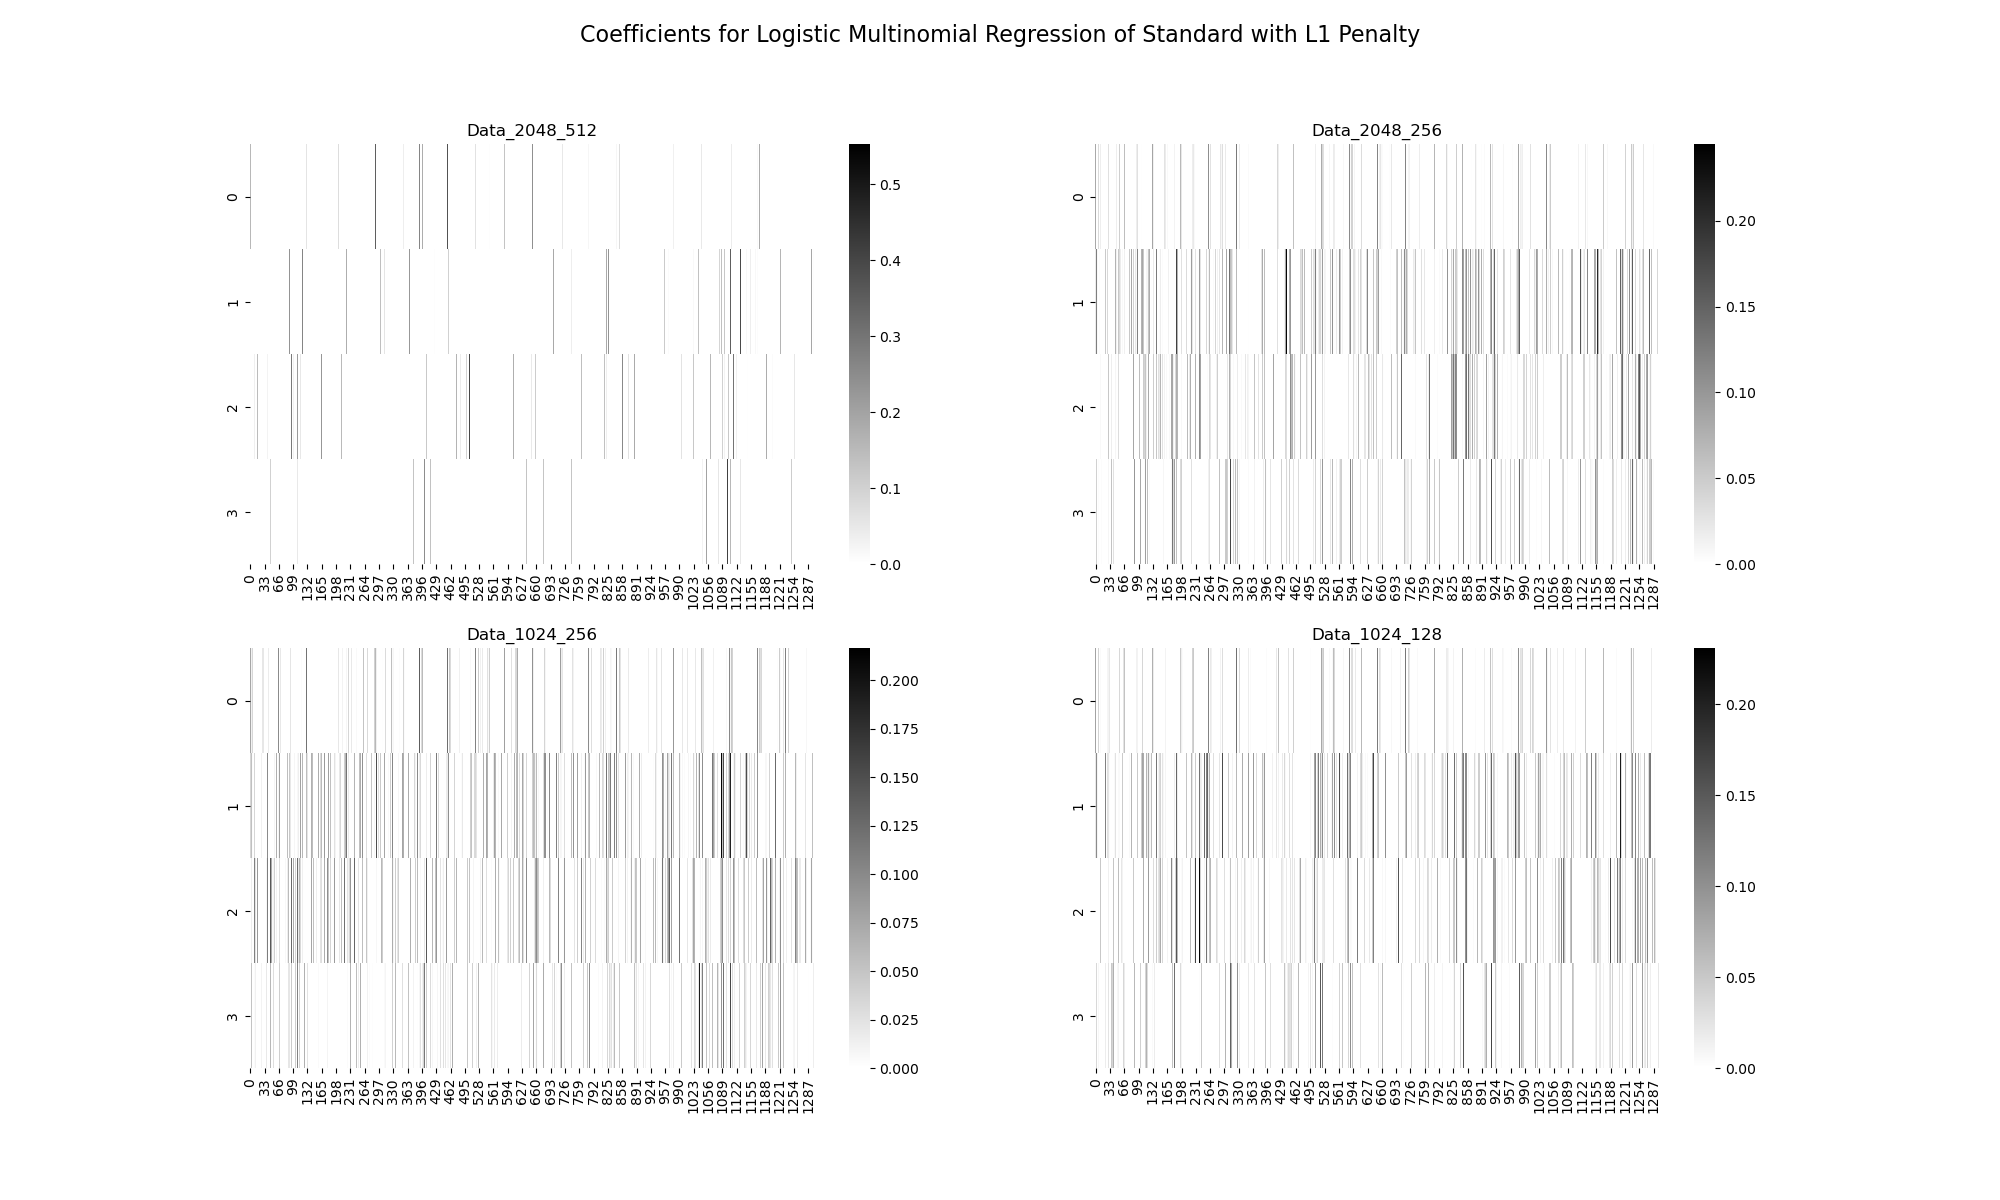
\includegraphics[width=0.9\linewidth]{../Statistical_Sciences_template/figure/Coefficients for Logistic Multinomial Regression of Standard with L1 Penalty.png}
	\caption{Coefficients for Multinomial Logistic Regression of Standard Datasets with L1 Penalty}
	\label{fig:MLRstdcoef}
\end{figure}
\noindent According to the numbers of the non-zero regression coefficients, we can further find that in the model of the dataset with frame length 2048 and hop length 512, the variables corresponding to non-zero coefficients show obvious differences: the most representative features of MFCCs' mean occupies a dominant position, with a total of 67 corresponding variables obtaining non-zero coefficients; followed by features related to the range, with 37 variables retained by the model, 42 variables corresponding to skewness, and 38 variables corresponding to kurtosis; in contrast, the variance feature describing the degree of dispersion performed the worst, with only 22 related variables selected by the model. In contrast, the model with the best results on the dataset with frame length 1024 and hop length 128, in which mean of MFCCs has a total of 335 related variables obtaining non-zero coefficients. The importance ranking of other statistics' types is consistent with the dataset with frame length 2048 and hop length 512, but the number scale has been significantly expanded: 274 variables of the range are retained, 286 of the skewness, and 288 of the kurtosis. The relative importance of the variance feature is still the lowest, with a total of 180 non-zero coefficients.\\
\\
Through comparative analysis of these models, we can draw the following important conclusion: first, the mean of MFCC shows the strongest discriminative ability among all statistics' types. This phenomenon may be due to the essential characteristics of the audio signal - the mean can effectively reflect the overall energy distribution of the signal, and this physical quantity often has a stable correlation with the audio category. Secondly, the performance of the variance feature is relatively weak. This may be because after standardization, the variance provides limited supplementary information, as larger variance means more information contained in data, hence the discriminative ability of variance is significantly weakened. Finally, although the statistics describing the distribution shape (skewness and kurtosis) and the value range are not as important as the mean, they still contain a considerable degree of discriminative information. These features can capture subtle differences in signal distribution and provide valuable supplementary information for the model.\\
\\
Figure \ref{fig:CMMLRstd} shows the confusion matrix performance of the best multinomial logistic regression model on the test set, where the category labels 0, 1, 2, and 3 correspond to classical, disco, hiphop, and metal respectively. Several important classification patterns can be observed from the confusion matrix: first, in the classical music category, the model shows perfect classification performance, and all test samples are correctly identified, which verifies the results in Section \ref{subsec:performance}. Second, the model only makes a few misclassifications between disco and hiphop, and between hiphop and mental, with only 3 observations misclassified in each case. However, the model has systematic biases in certain specific categories: for disco, the model shows a clear tendency to misclassify it as mental, with a total of 5 disco samples misclassified as mental. It is worth noting that this misclassification is asymmetric - there is no misclassification at all in the opposite direction (i.e. misclassifying mental as disco). This specific misclassification pattern directly affects the performance of the model's evaluation indicators: on the one hand, the recall of the disco is relatively lower because some of real disco samples are not correctly identified; on the other hand, the precision of the mental is also negatively affected because samples predicted as mental are mixed with samples that should belong to disco. This finding is completely consistent with the model performance indicators reported in Table \ref{table:best}.
\begin{figure}[H]
	\centering
	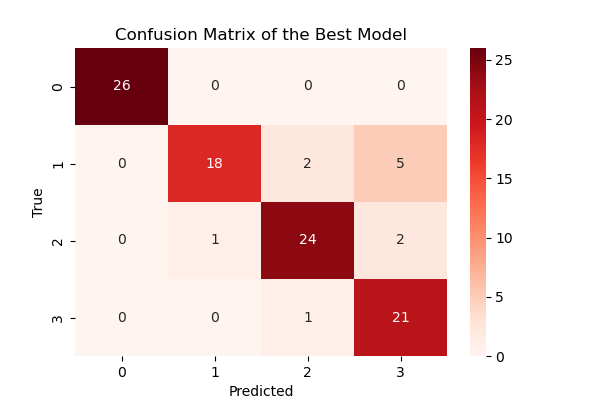
\includegraphics[width=0.9\linewidth]{../Statistical_Sciences_template/figure/Confusion matrix of the Best Model.png}
	\caption{Confusion matrix of the Best Model}
	\label{fig:CMMLRstd}
\end{figure}
\noindent For comparison, Figure \ref{fig:MLRcoef} shows a heat map of all coefficients in the multinomial logistic regression model based on unstandardized datasets. Through intuitive comparison, it can be found that the density of non-zero coefficients in Figure \ref{fig:MLRcoef} is significantly higher than that in Figure \ref{fig:MLRstdcoef}, which indicates that under unstandardized data conditions, the model tends to retain more variables. The results of the specific analysis of the dataset with frame length 1024 and hop length 128 show that variables related to the mean dominate the model, with a total of 1028 variables retained; since the data is not standardized, the importance of variance and range is also fully reflected in the model, of which 1037 non-zero coefficient variables corresponding to variance and 1031 corresponding to range. This shows that the number of variables corresponding to the three types of statistics, mean, variance and range, retained in the model is basically the same, the difference in the number of retained variables is less than 1\%, and their importance to the model is also relatively close. It is worth noting that the importance of skewness is significantly reduced, with only 68 related variables retained; while the number of variables corresponding to the kurtosis statistic is between the above two, with a total of 610 retained. This distribution pattern indicates that under unstandardized data conditions, the second-order moment statistics has a much greater impact on the model than higher-order statistics (i.e. skewness and kurtosis), which may be related to the original scale difference of the data.\\
\\
\begin{figure}[H]
	\centering
	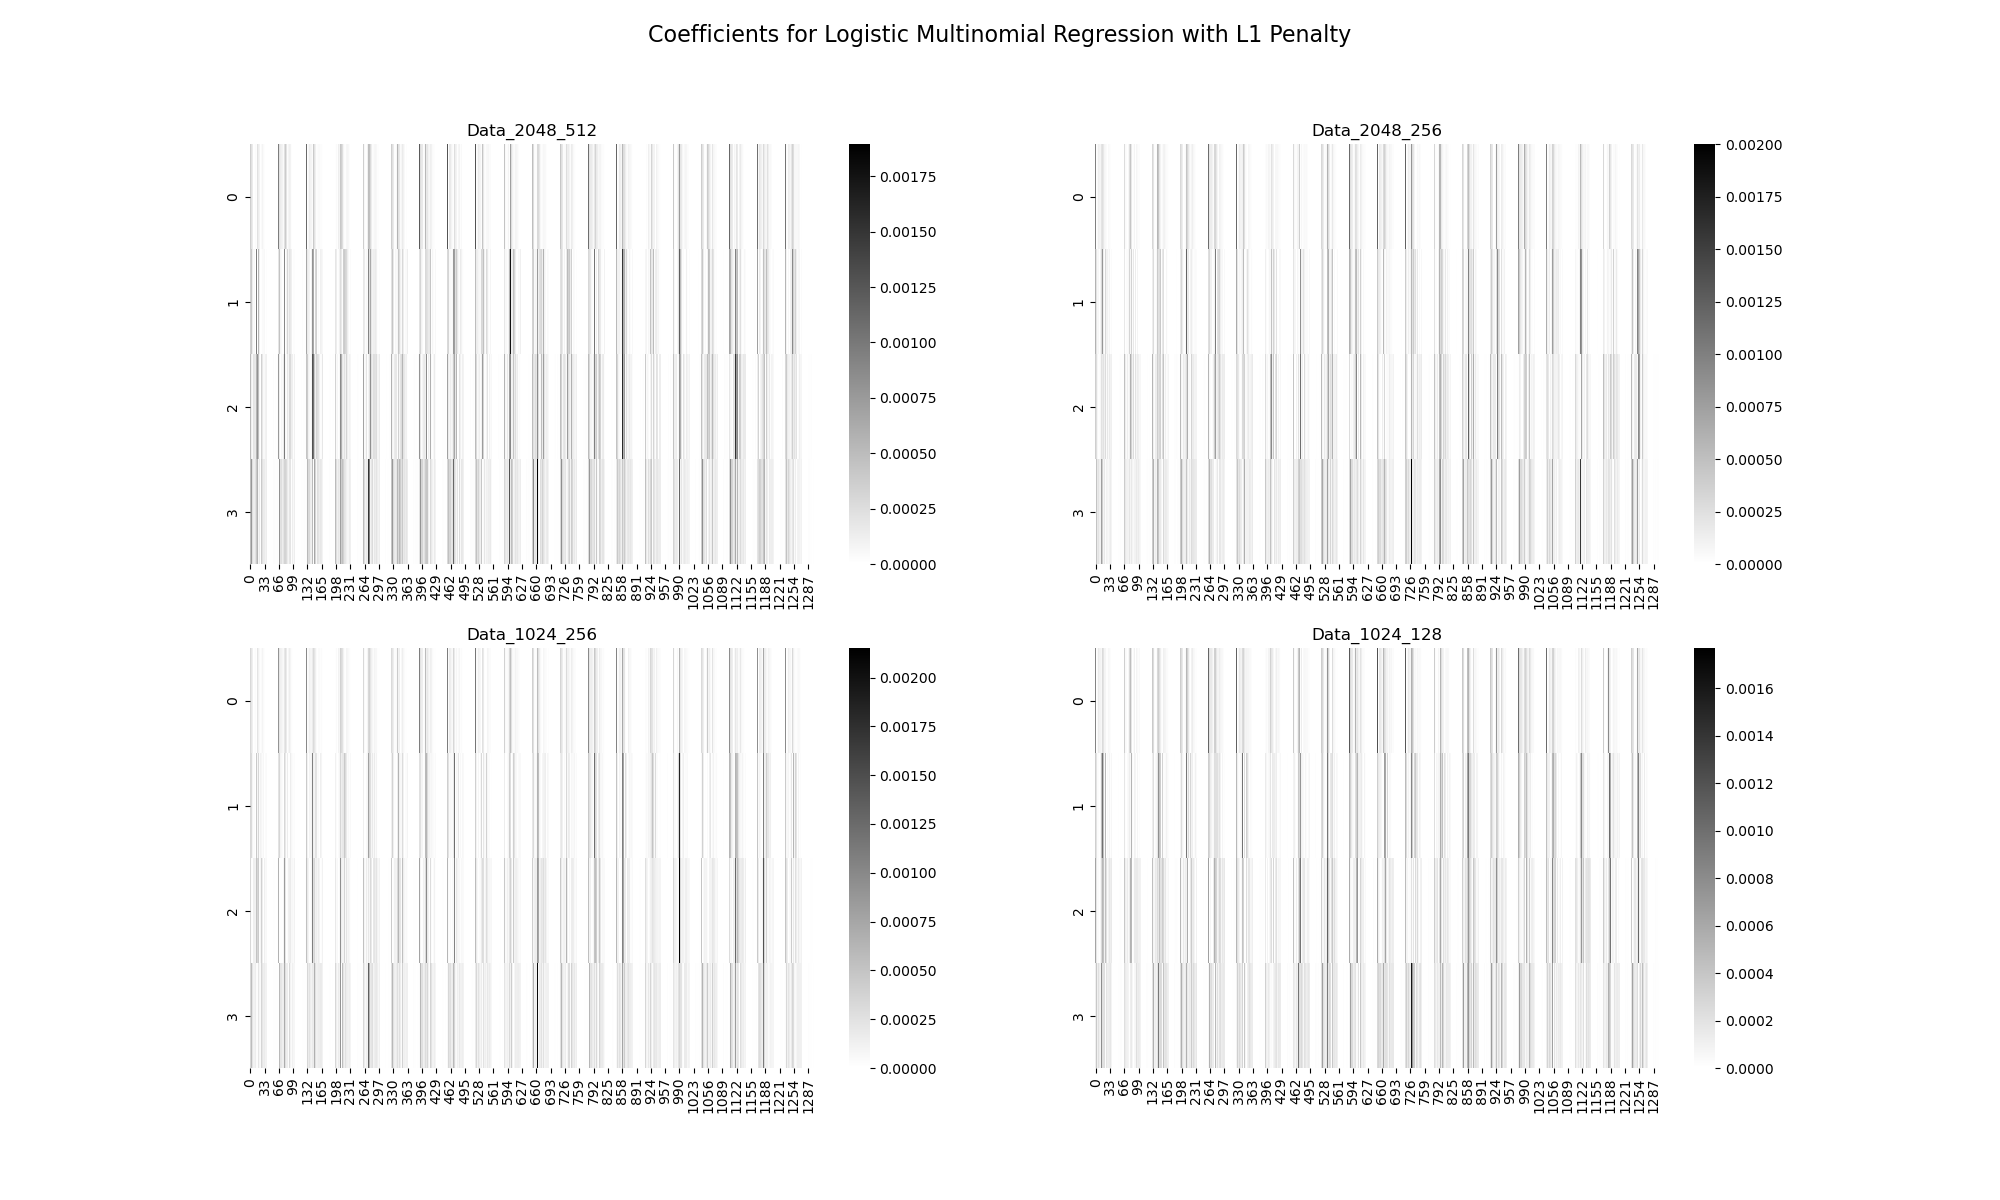
\includegraphics[width=0.9\linewidth]{../Statistical_Sciences_template/figure/Coefficients for Logistic Multinomial Regression with L1 Penalty.png}
	\caption{Coefficients for Logistic Regression of Unstandard Datasets with L1 Penalty}
	\label{fig:MLRcoef}
\end{figure}
\noindent From the performance comparison in Table \ref{table:L1penalty}, it can be seen that the models based on the unstandardized datasets performed significantly worse than the models based on the standardized datasets. Although more non-zero variables are retained in the unstandardized models, its prediction effect is worse, which may be mainly due to the fact that too many variables corresponding to variance are retained in the model. These variables are likely to be associated with noise, thus affecting the model performance. From the perspective of signal processing, STFT is used when calculating MFCCs, while STFT is based on the short-time stationarity assumption, that is, the second-order moment of the signal in the short-time window is required to remain constant. However, in actual situations, under the condition of unstandardized data, a large number of variables of MFCCs corresponding to variance are retained in the model, which not only squeezes out the importance of other statistical variables, but also these variables themselves may not contain enough information, but may introduce noise interference, ultimately leading to a decrease in model performance. In addition, due to the inconsistent scale of unstandardized data, some variables may be given higher weights simply because of their larger numerical range, rather than having stronger discrimination ability.\\
\\
In contrast, standardization achieves the unification of data scales, allowing the model to more effectively retain discriminative variables. This processing method eliminates the impact of dimensional differences between different features, allowing the model to more accurately capture the inherent laws of the data, thereby significantly improving the model's predictive performance. Standardized data allows various statistics to be compared at the same scale, avoiding unreasonable weights for certain features due to their large dimensions, and ensuring the objectivity and effectiveness of model learning. In addition, the standardization process may also suppress the interference of noise variables, allowing truly discriminative high-order statistics (i.e. skewness and kurtosis) to be more reasonably weighted in the model.\\
\\
Figure \ref{fig:SVMcoef} shows the heatmap of coefficients when SVM constructs a classification hyperplane in the feature space. Compared with the aforementioned regression model, these hyperplane coefficients show more sparse characteristics, but it is worth noting that the absolute values of non-zero coefficients are generally larger, and some coefficients even reach 0.3. This phenomenon is contrast to the regression model on the standardized data set, where the absolute values of regression coefficients on other datasets except the dataset with frame length 5048 and hop length 512 generally do not exceed 0.2. Further analysis shows that in the SVM model, the variables corresponding to the skewness and kurtosis statistics show stronger discrimination and importance. Taking the specific analysis of dataset with frame length 1024 and hop length 128 as an example, the number of non-zero coefficients related to skewness reaches 137, the number of non-zero coefficients related to kurtosis is 113, and the number of non-zero coefficients corresponding to mean, variance and range is significantly reduced, only 56, 46 and 53 respectively. This distribution pattern is essentially different from the results of the regression model: in regression analysis, variables corresponding to mean always dominate, but in the SVM classification task, high-order statistics (skewness and kurtosis) show stronger discrimination.\\
\\
\begin{figure}[H]
	\centering
	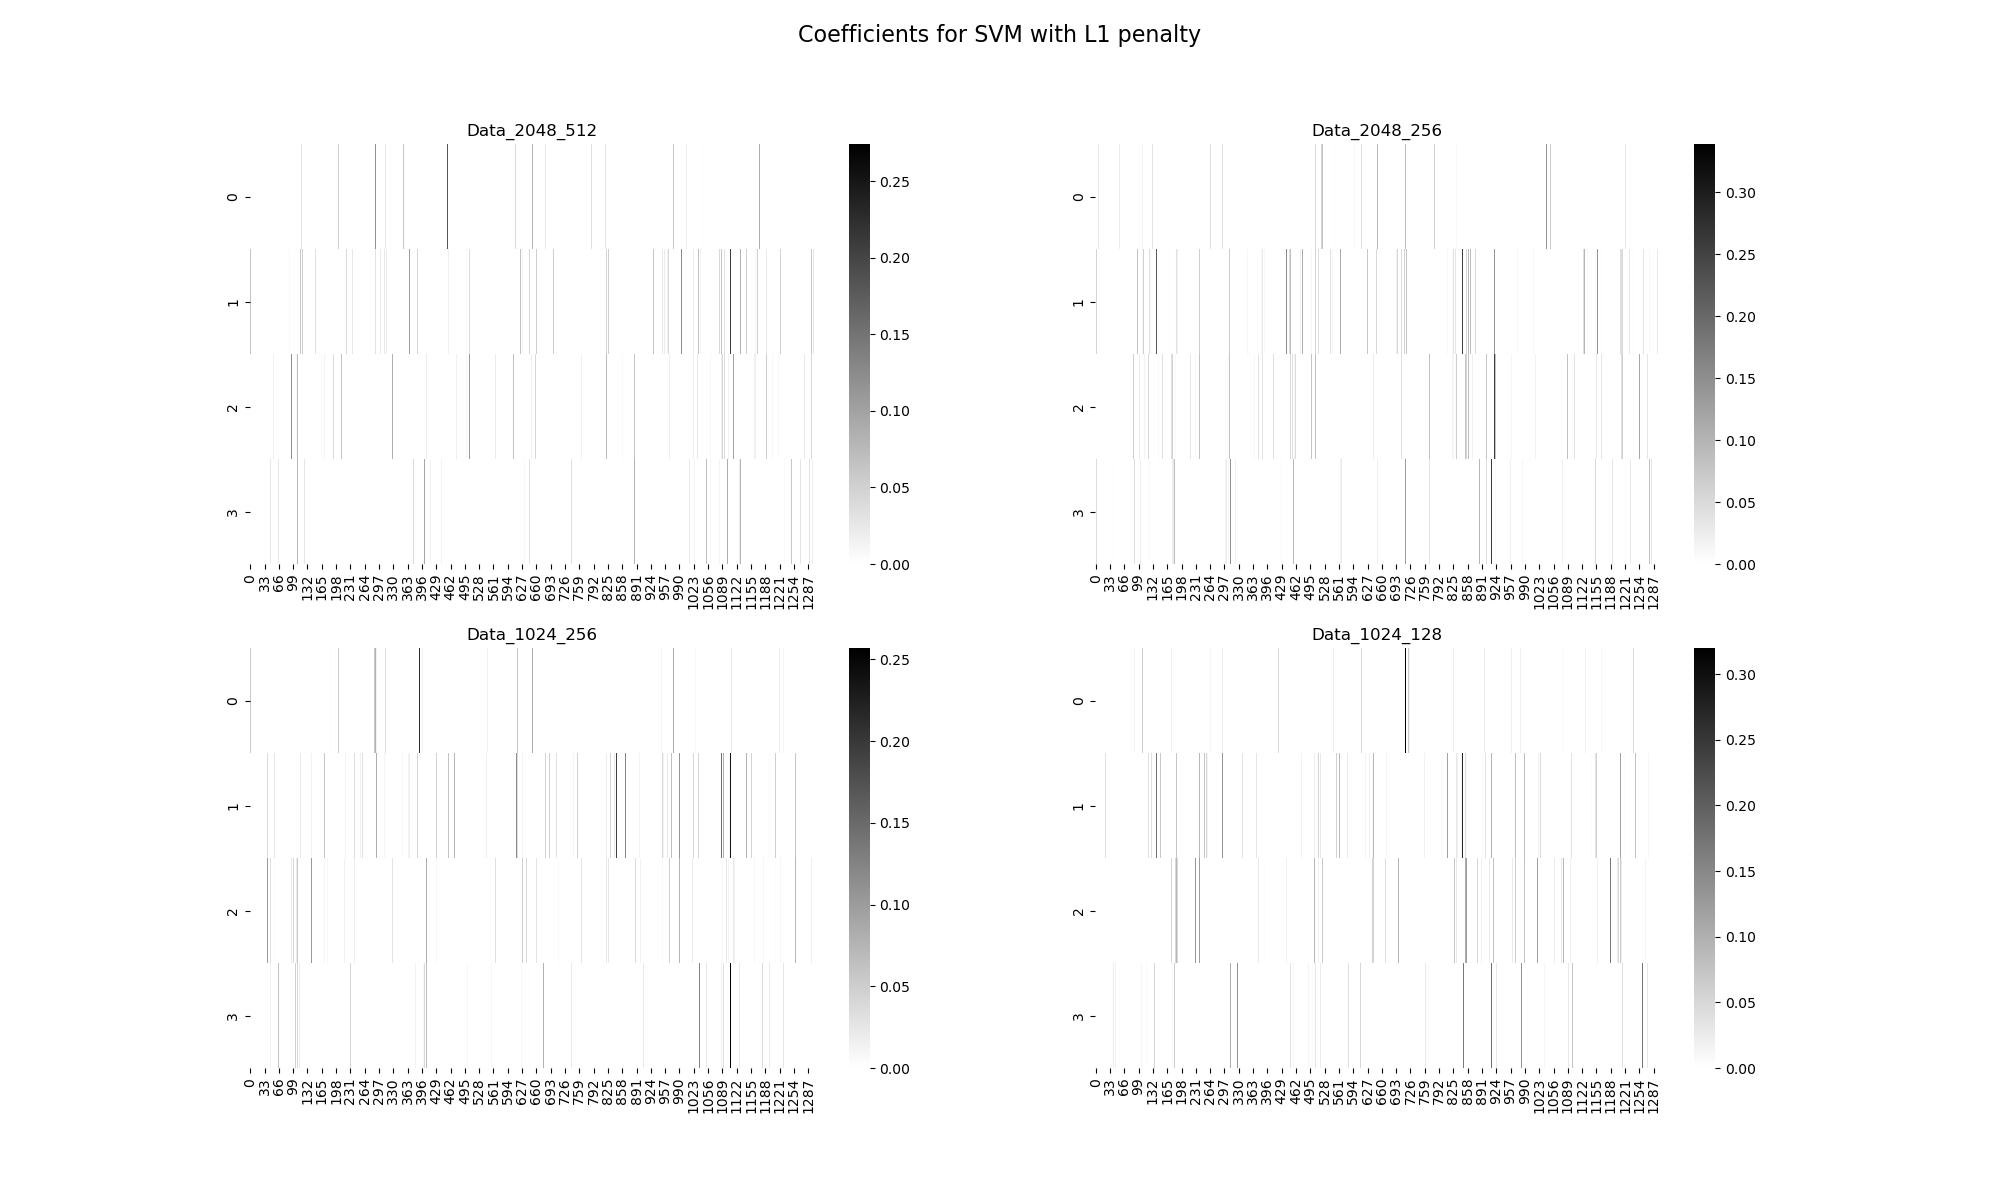
\includegraphics[width=0.9\linewidth]{../Statistical_Sciences_template/figure/Coefficients for SVM with L1 penalty.png}
	\caption{Coefficients for SVM with L1 penalty}
	\label{fig:SVMcoef}
\end{figure}
\noindent The best shapelet tree-based model constructed on the dataset with frame length 2048 and hop length 256 forms a decision tree structure with a depth of 3 as shown in Figure \ref{fig:shapelettree}. It can be clearly observed from the confusion matrix shown in Figure \ref{fig:CMshapelet} that the model has the best prediction performance for the classical, with only 3 observation samples being misclassified. In contrast, although the model has shown a certain degree of discrimination ability for the hiphop and mental, its prediction accuracy is lower than that of the classical category. It is particularly noteworthy that the model performs extremely poorly in the recognition of the disco, and is almost unable to effectively distinguish this category from other music types. This phenomenon can be explained by an in-depth analysis of the correspondence between the shapelet features shown in Figure \ref{fig:shapelets} and the time series of each category.\\
\\
\begin{center}
	\begin{tikzpicture}[
        level 1/.style={sibling distance=6cm, level distance=1.5cm},
        level 2/.style={sibling distance=4cm, level distance=1.5cm},
        level 3/.style={sibling distance=2cm, level distance=1.5cm},
		every node/.style={draw, rectangle}
		]
		\node (Root) {all}
		child {node {Classical}
		}
		child {node {}
			child {node {}
				 child {node {Hiphop}}
				 child {node {Disco}}
			}
			child {node {} 
				child {node {Mental}} 
				child {node {Hiphop}}
			}
		};
	\end{tikzpicture}
	\label{fig:shapelettree}
\end{center}
\noindent The shapelet used by the parent node corresponds to the red curve in Figure \ref{fig:shapelets} that shows a fishhook shape. This feature has a large time span and significant amplitude changes. By comparing the time series features of each category, it can be found that classical music shows extremely significant amplitude fluctuations in the time period corresponding to this shapelet, especially in the low-frequency area (the part with lower values). This unique fluctuation pattern makes the distance measurement value between the classical music sequence and the fishhook shapelet significantly smaller than that of other categories, thus forming an effective basis for discrimination.\\
\\
\begin{figure}[H]
	\centering
	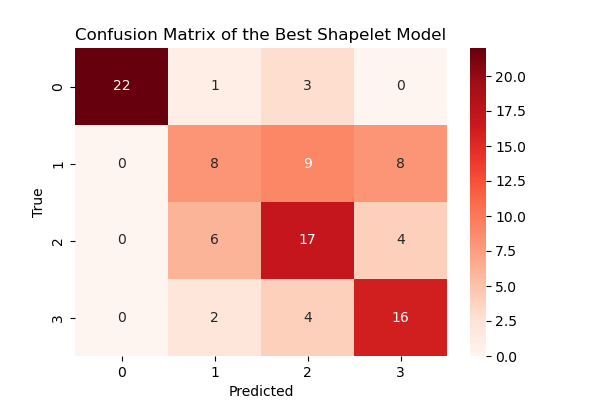
\includegraphics[width=0.9\linewidth]{../Statistical_Sciences_template/figure/Confusion matrix of the Best Shapelet Model.png}
	\caption{Confusion matrix of the Best Shapelet Model}
	\label{fig:CMshapelet}
\end{figure}
\noindent Further analysis of the discriminant features of the third layer of the decision tree shows that the shapelet used by the right child node (corresponding to the red curve starting from -57 and with a length of 9 time units in Figure \ref{fig:shapelets}) has a certain effect in distinguishing hiphop and mental categories. This shapelet is closer to the time series morphology of hiphop music, but has a more obvious morphological difference with the mental category. However, the shapelet used by another third-layer child node (corresponding to the red curve starting from -25 and with a length of 9 time units in Figure \ref{fig:shapelets}) shows poor representativeness. This feature is morphologically between the hiphop and disco categories and cannot form an effective discriminant boundary, which directly leads to the model's serious lack of recognition ability for the disco category. From the perspective of time series morphology, the distribution of disco music in this feature space has a large overlap with other categories, and lacks a unique and discriminative fluctuation pattern, which is the fundamental reason for the model's disastrous results in this category.
\begin{figure}[H]
	\centering
	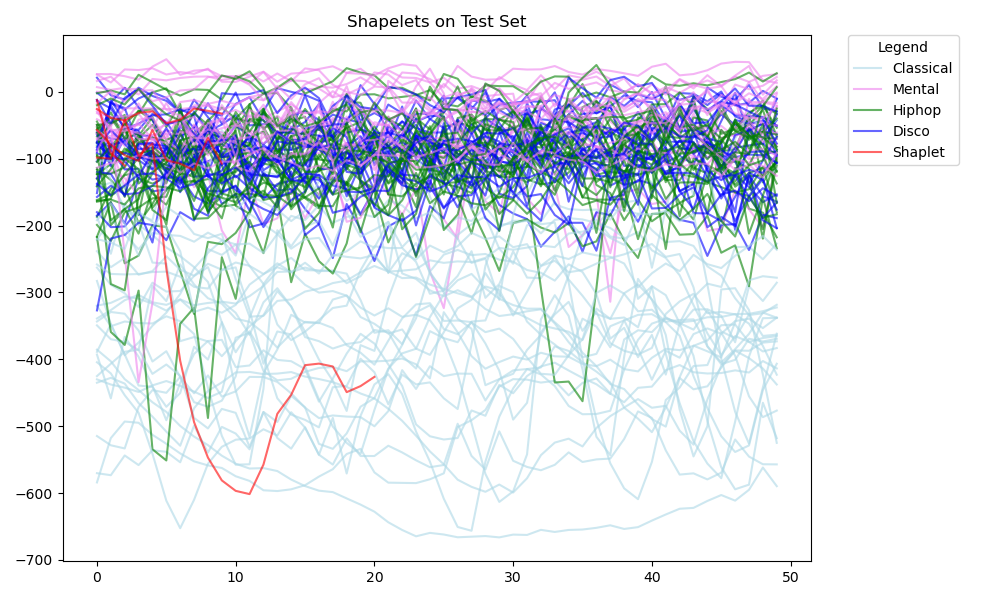
\includegraphics[width=0.9\linewidth]{../Statistical_Sciences_template/figure/Shapelets on Test Set.png}
	\caption{Shapelets and the Samples from Test Set}
	\label{fig:shapelets}
\end{figure}

\chapter*{Conclusions}
\addcontentsline{toc}{chapter}{Conclusions}
Mel-frequency cepstral coefficients (MFCC) have shown powerful capabilities in the task of automatic music classification, mainly due to their high simulation of human auditory characteristics and accurate extraction of key features of music signals. MFCC effectively captures the perceptual features related to pitch and timbre in music by converting the spectrum into a nonlinear frequency domain representation based on the Mel scale, and is particularly suitable for processing the non-stationary characteristics of music signals. The pre-emphasis, framing, and windowing steps included in its calculation process can effectively suppress the interference of environmental noise and recording differences, while the cepstral coefficients extracted by discrete cosine transform (DCT) focus on the macroscopic features of the spectrum envelope, which happens to be highly consistent with the key information such as harmonic structure and resonance peak distribution relied on in tasks such as music style and instrument classification. In addition, the low-dimensional characteristics of MFCC significantly reduce the computational complexity, allowing it to be efficiently combined with machine learning models. This experiment shows that in the classification tasks of genres such as classical, hip-hop, mental, and disco, the classification accuracy of MFCC features is relatively high. This feature representation that takes into account both physiological perception principles and mathematical simplicity makes it one of the enduring basic features in the field of music information retrieval.\\
\\
Although the shapelet tree-based algorithm has shown certain effectiveness in specific music classification tasks, its applicability has obvious limitations. The algorithm can achieve good classification results for some music categories (such as classical), but its ability to distinguish other categories (such as disco) is relatively weak. The root cause of this phenomenon may be the complex humanistic attributes of the music genre classification itself. The division of music genres is essentially an artificially constructed classification system, and its formation process is deeply influenced by multiple factors such as historical culture, social changes, and artistic creation practices, rather than simply determined by the physical characteristics of audio signals. From the historical dimension of music development, there is often a complex relationship of integration and evolution between different genres. Many music genres borrow from each other and influence each other during their formation, resulting in the fact that there may not be absolutely clear boundaries between them in terms of audio features. In addition, musicians of different genres often use similar instrument combinations, and the overlap of instrument use further increases the difficulty of classification based on audio features. Specifically speaking of the limitations of MFCC features, it may be difficult to fully capture the essential differences between music genres by relying solely on the MFCC coefficients in the low-frequency band. Although MFCC can effectively characterize the spectral envelope characteristics of audio signals, it mainly reflects the physical properties of sound, while the distinction between music genres often involves higher-level musical elements, such as harmony, rhythmic patterns, and performance techniques. These musical elements may not be fully expressed in the low-dimensional MFCC feature space.\\
\\
Based on the above analysis results, the application of shapelet tree-based algorithm in music genre classification task should not be limited to single-dimensional time series analysis, but should be extended to multi-dimensional time series analysis. This study of this experiment shows that it is difficult to achieve effective classification of certain music categories (such as disco) by relying only on one-dimensional MFCC coefficients in low-frequency bands. This limitation is largely due to the fact that the feature representation of a single dimension cannot fully reflect the complex characteristics of music signals. From the perspective of signal processing, music is a complex acoustic signal, and the information contained in different frequency bands is significantly different: low-frequency components mainly reflect the rhythm and basic harmonic structure of music, mid-frequency bands often contain the timbre characteristics of human voices and main instruments, and high-frequency components may carry information such as detailed texture and spatial sense of music. Therefore, future research should focus on exploring how to use MFCC coefficients in the full frequency domain to build a more effective classification model. Specifically, it is possible to consider processing MFCC coefficients of different frequency bands as interrelated multi-dimensional time series, and to mine more discriminative music features by analyzing the synergistic change pattern of the characteristics of each frequency band. For example, some music genres may exhibit unique energy distribution patterns or dynamic change characteristics in specific frequency bands (such as mid-high frequencies), which may be completely ignored in a single low-frequency analysis. In addition, the correlation between features in different frequency bands may also contain important genre distinguishing information: classical music may show coordinated changes in energy in each frequency band, while electronic music may show prominent periodic fluctuations in specific frequency bands. At the technical implementation level, the multidimensional shapelet tree algorithm needs to consider how to effectively deal with the computational complexity of high-dimensional time series data. Developing a new multidimensional shapelet extraction algorithm, changing the input one-dimensional time series to a multidimensional time series, can simultaneously consider the joint distribution characteristics of multiple frequency band features. Such improvements are expected to significantly enhance the model's ability to distinguish complex music genres.

\chapter*{Acknowledgements}
\addcontentsline{toc}{chapter}{Acknowledgements}
Studying at the Università di Bologna is an unforgettable and wonderful journey. First of all, I would like to express my sincere gratitude to my supervisor, Professor Matteo Farnè. Thank you for your professional guidance and valuable suggestions during the writing of my thesis. I have benefited a lot from your rigorous academic attitude and profound knowledge.\\
\\
At the same time, I would like to express my special thanks to my parents. Thank you for your selfless love and support over the years. It is your encouragement that allows me to devote myself to my studies and face every challenge bravely. Your trust has always been the source of my motivation to move forward.\\
\\
Finally, thank you to all the teachers, classmates and friends who have helped me in this academic journey. This precious experience will always be engraved in my memory.

\printbibliography
\addcontentsline{toc}{chapter}{References}

\appendix
\chapter{Appendix}
\section{Appendix: Instructions of Algorithm}\label{app:A}
The implementation of the shapelet tree-based algorithm is carried out in the Python script named "shapelet.py", which is located in the main\textunderscore program folder. This script contains all the core functions described in Section \ref{sec:algo}, including generate\textunderscore candidates, subsequence\textunderscore dist, CalculateInformationGain, check\textunderscore candidate, and find\textunderscore best\textunderscore shapelet. The program also defines a class named MultiTree, which serves as the main structure for the shapelet tree model. The functionality provided by this class is similar to that of a standard decision tree implementation. Specifically, it includes methods for fitting the model to a training dataset, storing the learned tree structure, printing the tree structure, and making predictions on new time series datasets. Following is the example how to use the class:\\
\begin{lstlisting}[language=Python, caption=Example of using the shapelet tree-based algorithm]
# set the parameters
mt=MultiTree(MAXLEN=20,MINLEN=3,max_depth=5,min_samples_split=5) 

# fit the model
mt.fit(train_series, original_label) 

# print the model structure	
mt.print_tree_structure() 

# assign the model structure to a variable	
structure=mt.get_tree_structure() 

# make predictions on new datasets	
y_pred=mt.predict(test_series) 
\end{lstlisting}
\section{Appendix: Information of GTZAN Dataset}\label{app:B}
The GTZAN dataset can be accessed through multiple platforms. On the TensorFlow Datasets catalog, it is available at \href{https://www.tensorflow.org/datasets/catalog/gtzan}{TensorFlowDatasets},
and on Kaggle at
\href{https://www.kaggle.com/datasets/andradaolteanu/gtzan-dataset-music-genre-classification}{Kaggle}.\\
\\
In addition to the raw audio files, the Kaggle distribution includes:
\begin{itemize}
	\item Waveform visualizations for each files (PNG images), which provide a quick way to view signal dynamics at a glance.
	\item Two CSV feature tables, one summarizing features computed over 3-second windows and another over the full 30-second duration. These tables contain commonly used audio features (e.g., spectral centroid, zero-crossing rate, MFCCs), ready for direct input into classification models.
\end{itemize}
But all the attached files above were not used in this study.\\
\\
The full dataset contains ten genres—blues, classical, country, disco, hiphop, jazz, metal, pop, reggae, and rock—with 100 files for each genre. One practical issue to note: in the Kaggle release, the file jazz.00054.wav is corrupted and cannot be read directly. Fortunately, this missing track can be retrieved from alternative sources (e.g., the original Marsyas repository or the TensorFlow mirror) to ensure the dataset remains complete.

\newpage
\section{Appendix: Codes for Statistical Models}\label{app:C}
All the codes are uploaded in Github:\\
\\
For the part of getting the features from audio signal, the codes are in the document named "feature project.py". For the part of clustering models and the visualization, the codes can be found in document "Visualisation and Clustering.py". Thus for the supervised models including the shapelet tree-based algorithm, the codes are in the document of "model.py".\\
\\


\end{document}
